\section{Eksperymenty}
W tym rozdziale opisane zostaną eksperymenty przeprowadzone w celu zbadania testów wydajnościowych środowisk uruchomieniowych. Testy zostały przeprowadzone na jednym komputerze wyposażonym w system operacyjny Linux, co pozwoliło na zminimalizowanie wpływu innych czynników na wyniki testów.

Testy wykorzystują wszystkie możliwe funkcjonalności, które są zaimplementowane w danych środowiskach. Dzięki czemu, testy te są odzwierciedleniem rzeczywistego zastosowania danego środowiska. Testy zostały wykonane w dwóch językach programowania: JavaScript oraz TypeScript. Zastosowanie tych języków pozwala na przetestowanie czasu potrzebnego do transpilacji kodu źródłowego do kodu maszynowego. 

\subsection{Algorytmy sortowania}
W celu zbadania wydajności danego środowiska uruchomieniowego, skonstruowana odpowiednie eksperymenty, które sprawdzają wydajność algorytmu sortowania. Wszystkie algorytmu sortowania zostały przetestowane dla każdego środowiska.

W tabeli \ref{tab:sorting_experiments} przedstawiono ilość iteracji oraz ilość eksperymentów dla przeprowadzonych eksperymenty.

\begin{table}[H]
  \centering
  \caption{Parametry eksperymentów - algorytmy sortowania}
  \begin{tabular}{|c|c|}
    \hline
    \textbf{Liczba eksperymentów} & \textbf{Liczba elementów} \\ \hline
    100 & 1000 \\ \hline
    1000 & 1000 \\ \hline
    100 & 10000 \\ \hline
    1000 & 10000 \\ \hline
  \end{tabular}
  \label{tab:sorting_experiments}
\end{table}

\subsubsection{Wyniki - sortowanie bąbelkowe}
Na rysunku \ref{fig:bubble_sorting_e1} przedstawiono wyniki eksperymentów dla algorytmu sortowania bąbelkowego dla 100 iteracji i 1000 elementów napisanego w języku JavaScript. Na wykresie przedstawiono czas wykonania jednorazowego testu w milisekundach oraz ilość zajmowanej pamięci w kilobajtach (kB).

\begin{figure}[H]
  \centering
  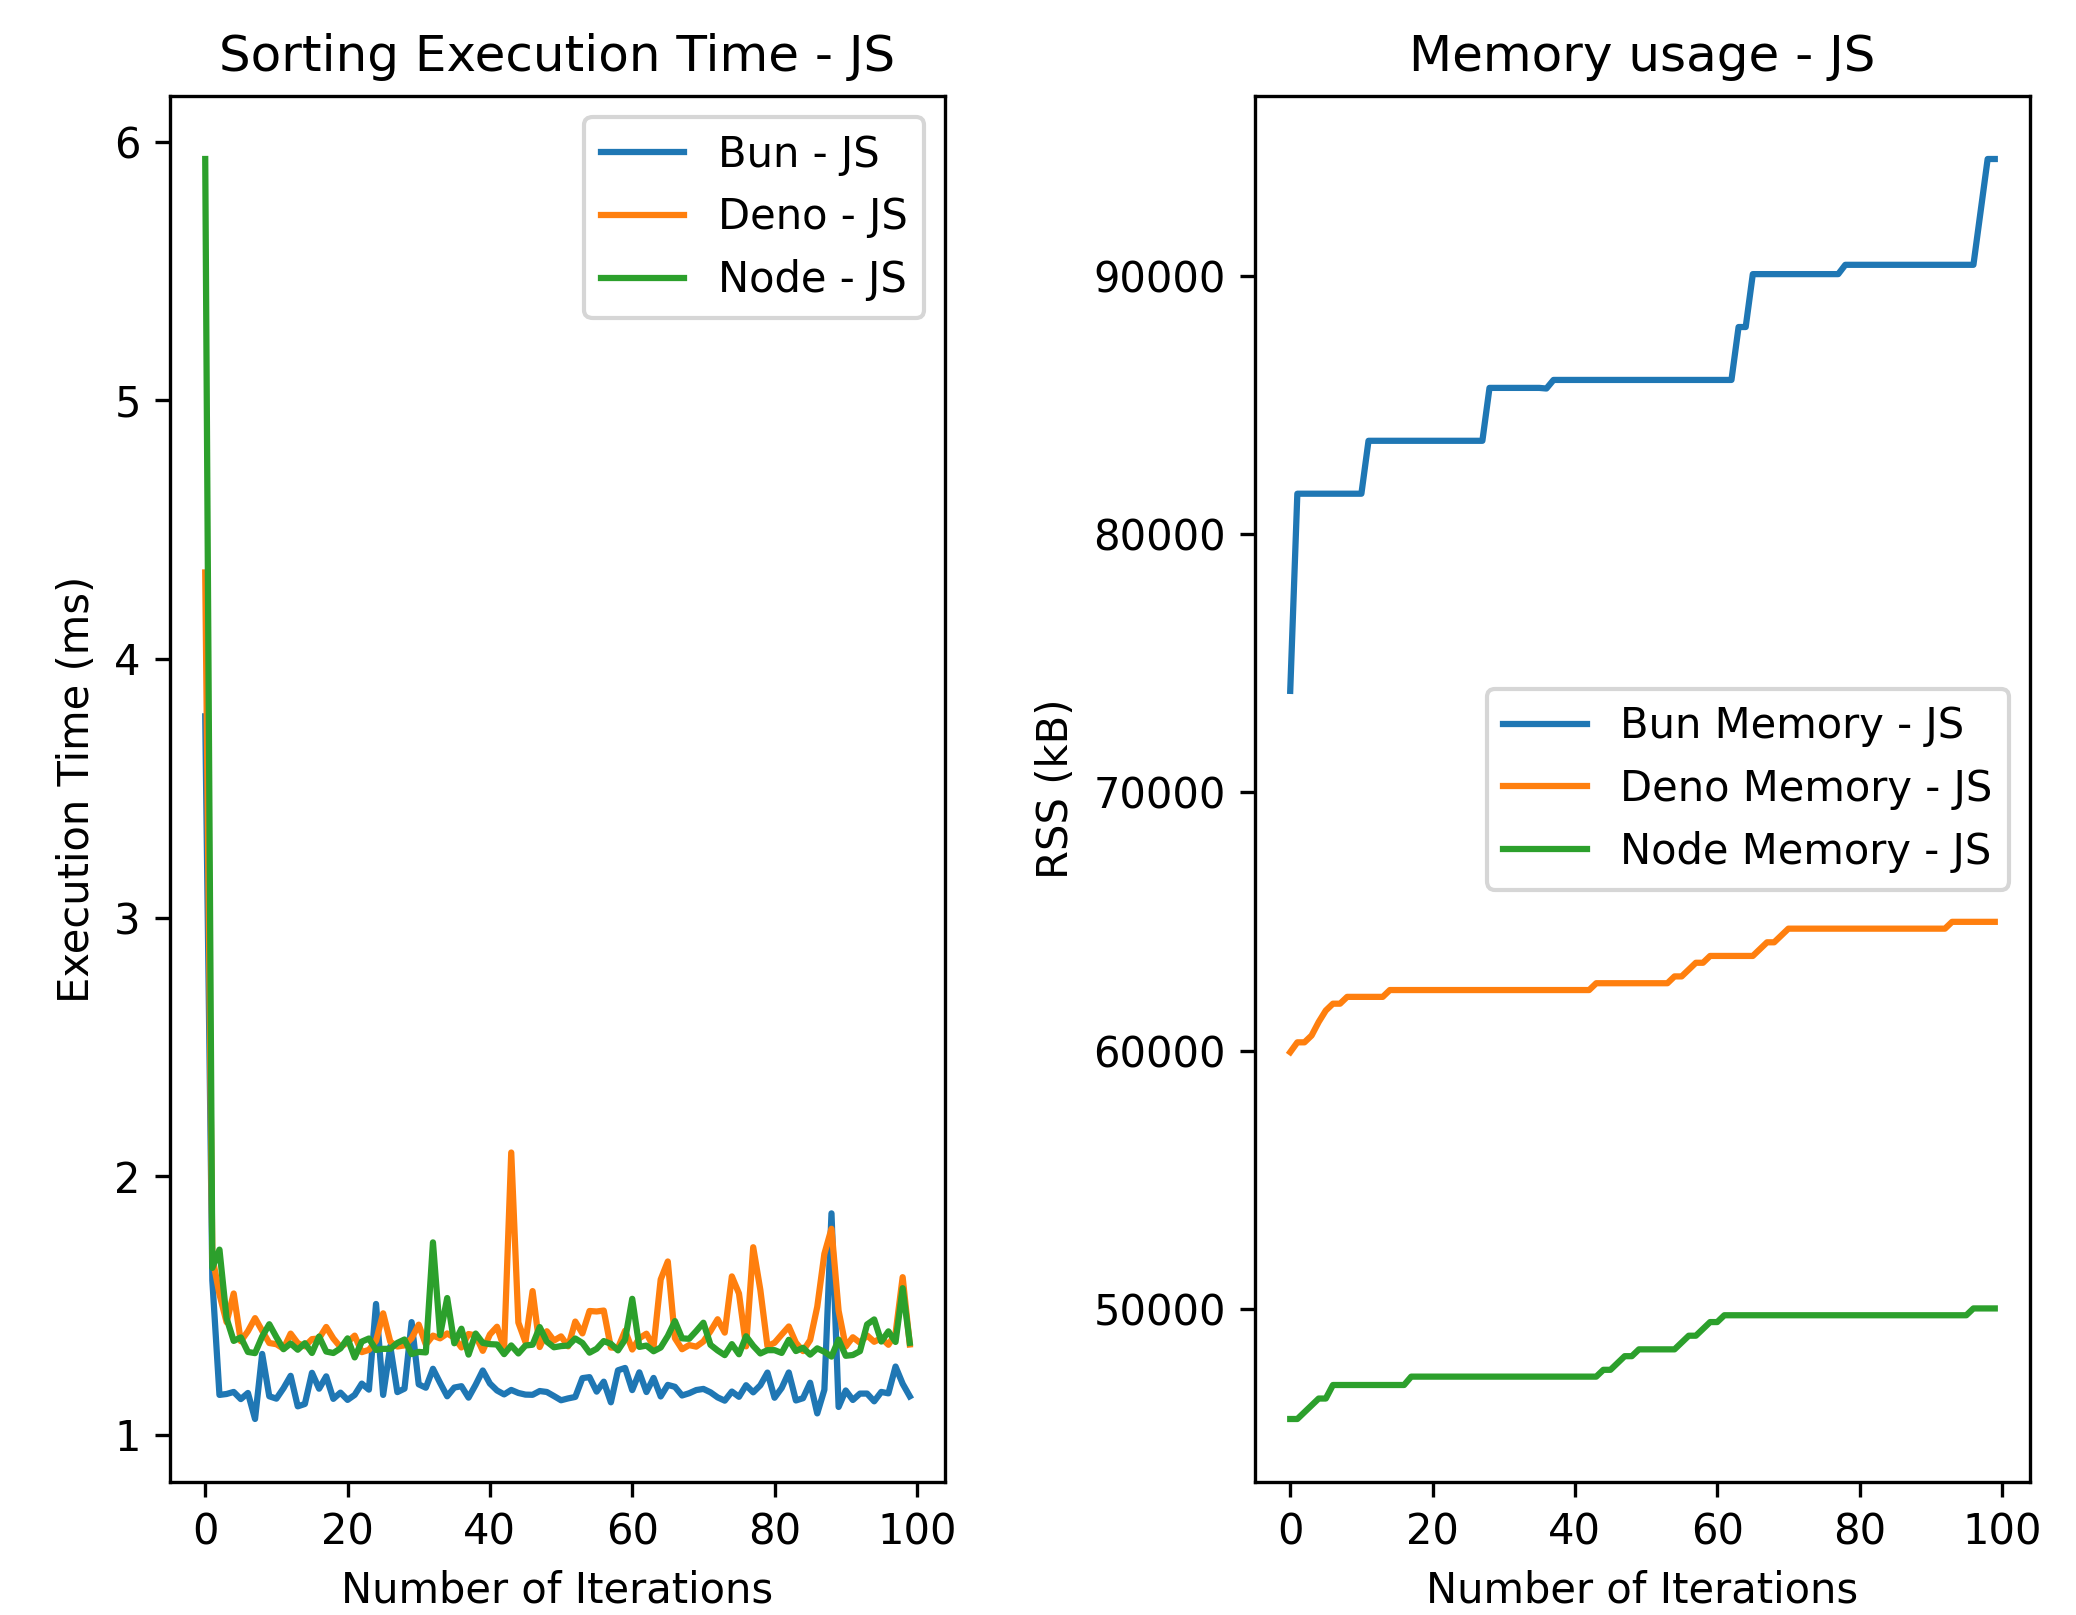
\includegraphics[width=0.7\textwidth]{Figures/sorting/sorting_bubble_100_1000_js.png}
  \caption{Wyniki eksperymentów dla algorytmu sortowania bąbelkowego dla 100 iteracji i 1000 elementów - po lewej czas wykonania jednorazowego testu w milisekundach, po prawej ilość zajmowanej pamięci w kilobajtach (kB)}
  \label{fig:bubble_sorting_e1}
\end{figure}

Na rysunku \ref{fig:bubble_sorting_e1_ts} przedstawiono wyniki eksperymentów dla algorytmu sortowania bąbelkowego dla 100 iteracji i 1000 elementów napisanego w języku TypeScript. Na wykresie przedstawiono czas wykonania jednorazowego testu w milisekundach oraz ilość zajmowanej pamięci w kilobajtach (kB).

\begin{figure}[H]
  \centering
  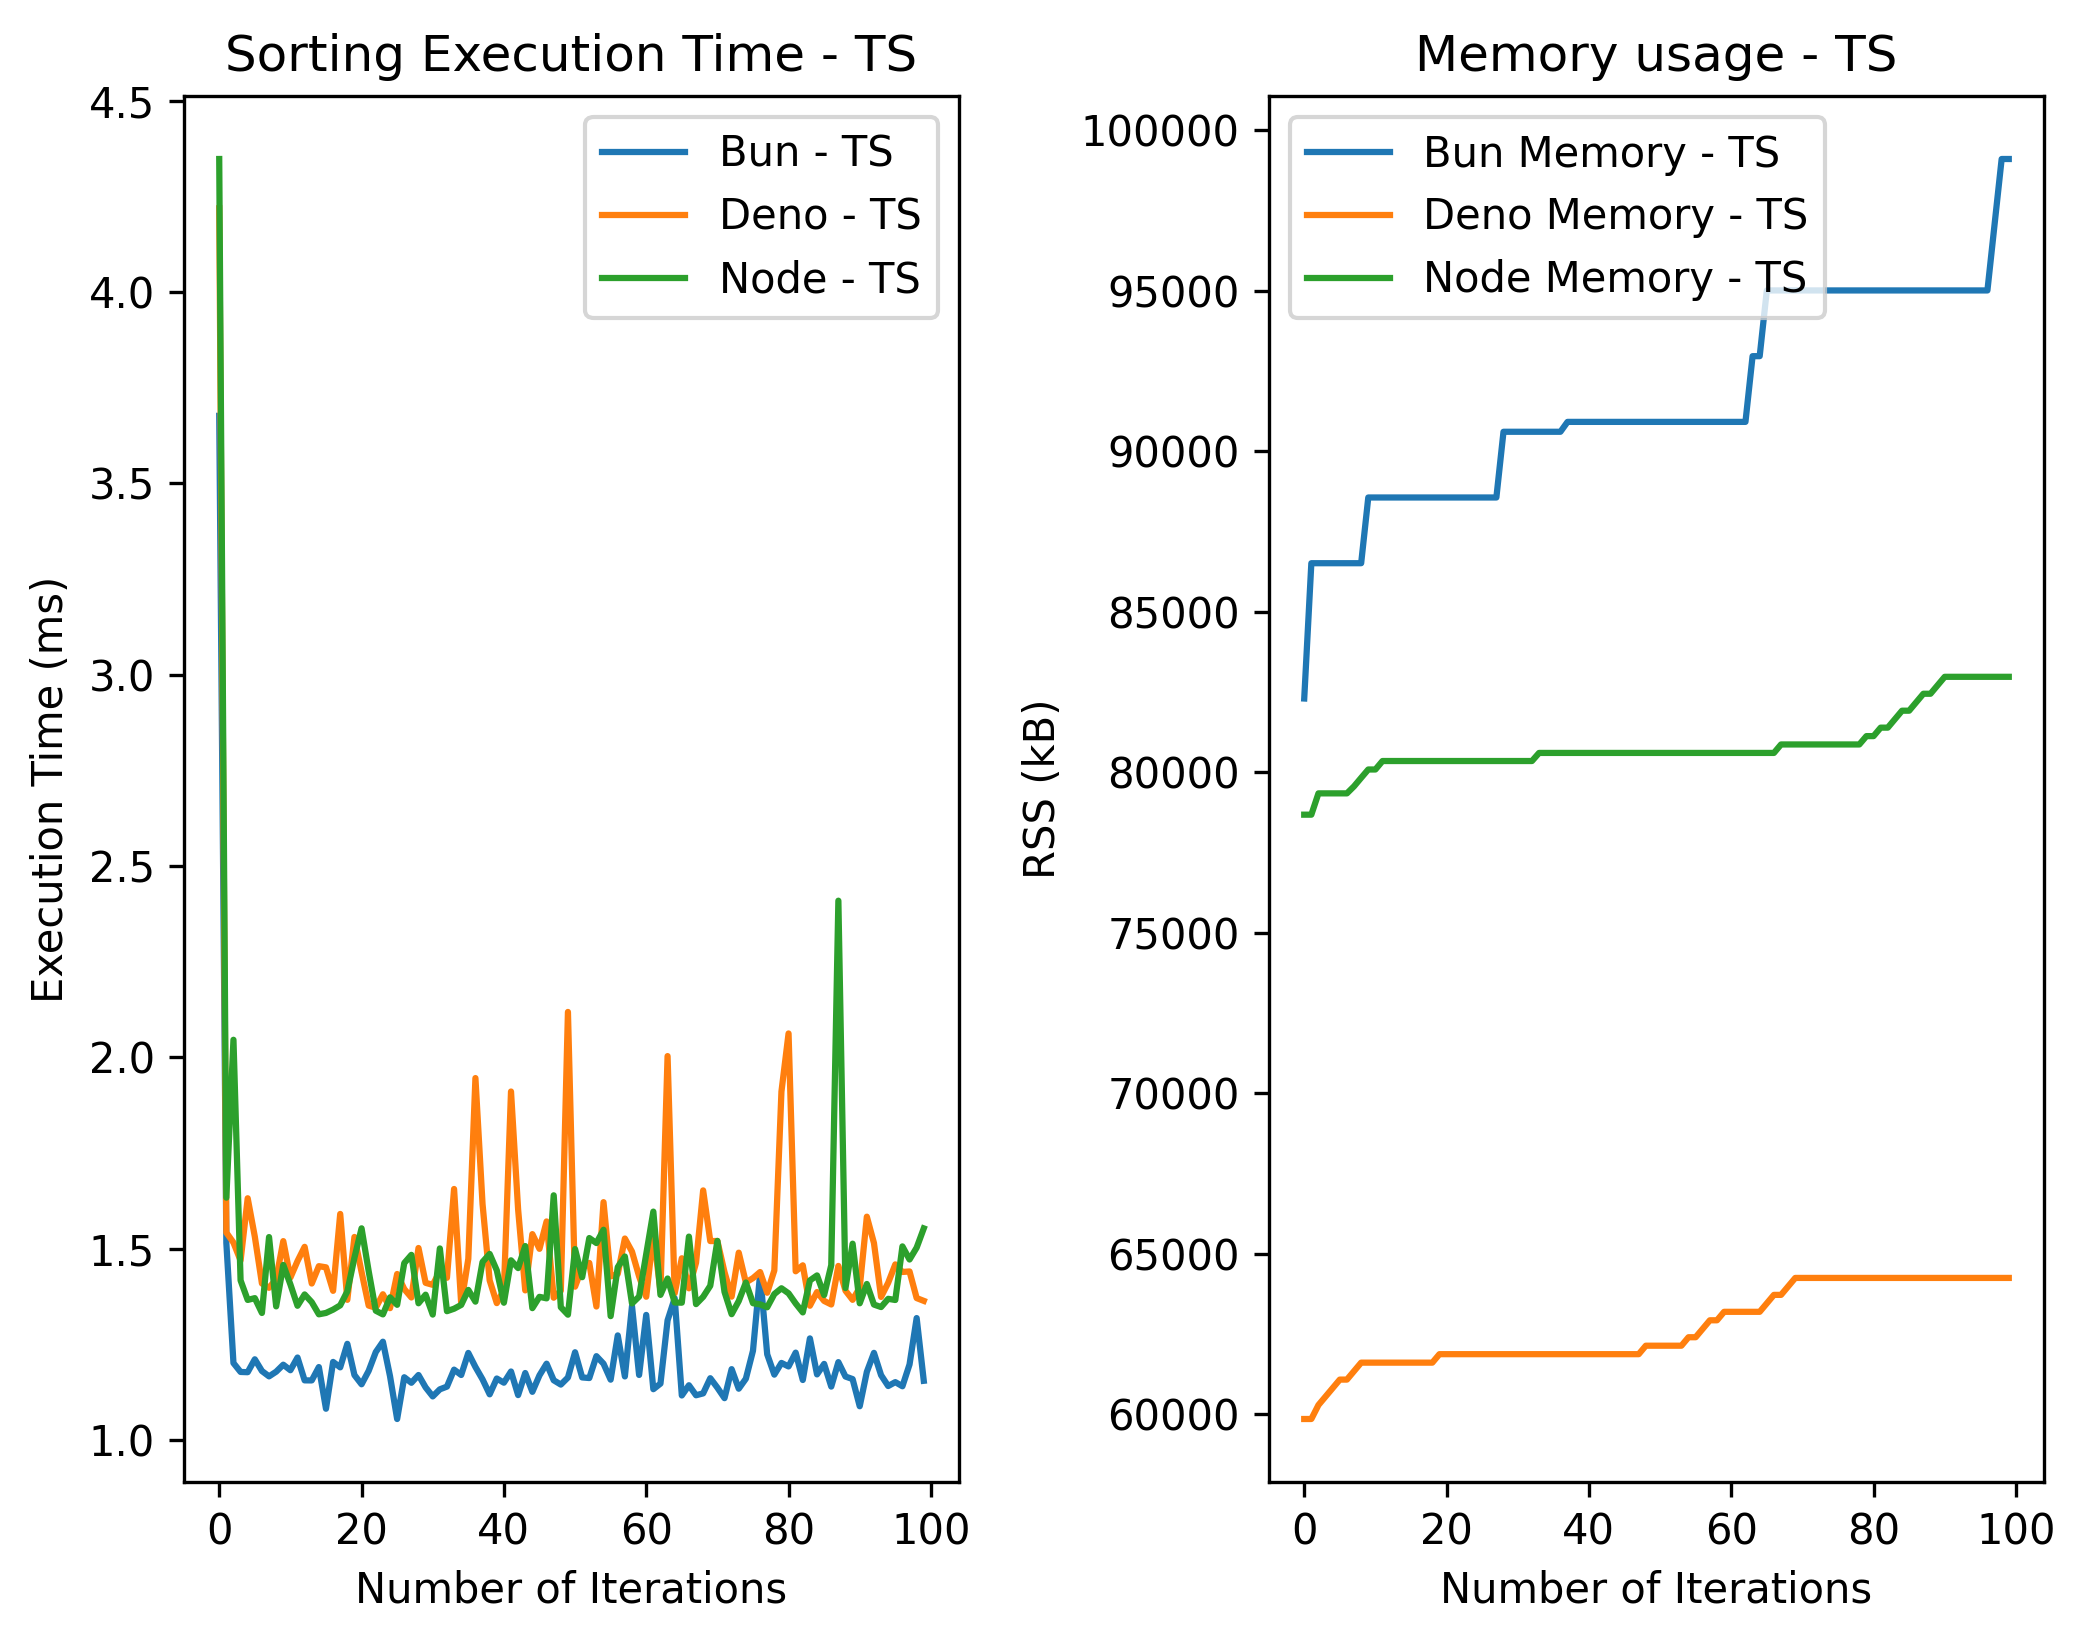
\includegraphics[width=0.7\textwidth]{Figures/sorting/sorting_bubble_100_1000_ts.png}
  \caption{Wyniki eksperymentów dla algorytmu sortowania bąbelkowego dla 100 iteracji i 1000 elementów - po lewej czas wykonania jednorazowego testu w milisekundach, po prawej ilość zajmowanej pamięci w kilobajtach (kB)}
  \label{fig:bubble_sorting_e1_ts}
\end{figure}

Na rysunku \ref{fig:bubble_sorting_e2} przedstawiono wyniki eksperymentów dla algorytmu sortowania bąbelkowego dla 100 iteracji i 1000 elementów napisanego w języku JavaScript. Na wykresie przedstawiono czas wykonania jednorazowego testu w milisekundach oraz ilość zajmowanej pamięci w kilobajtach (kB).

\begin{figure}[H]
  \centering
  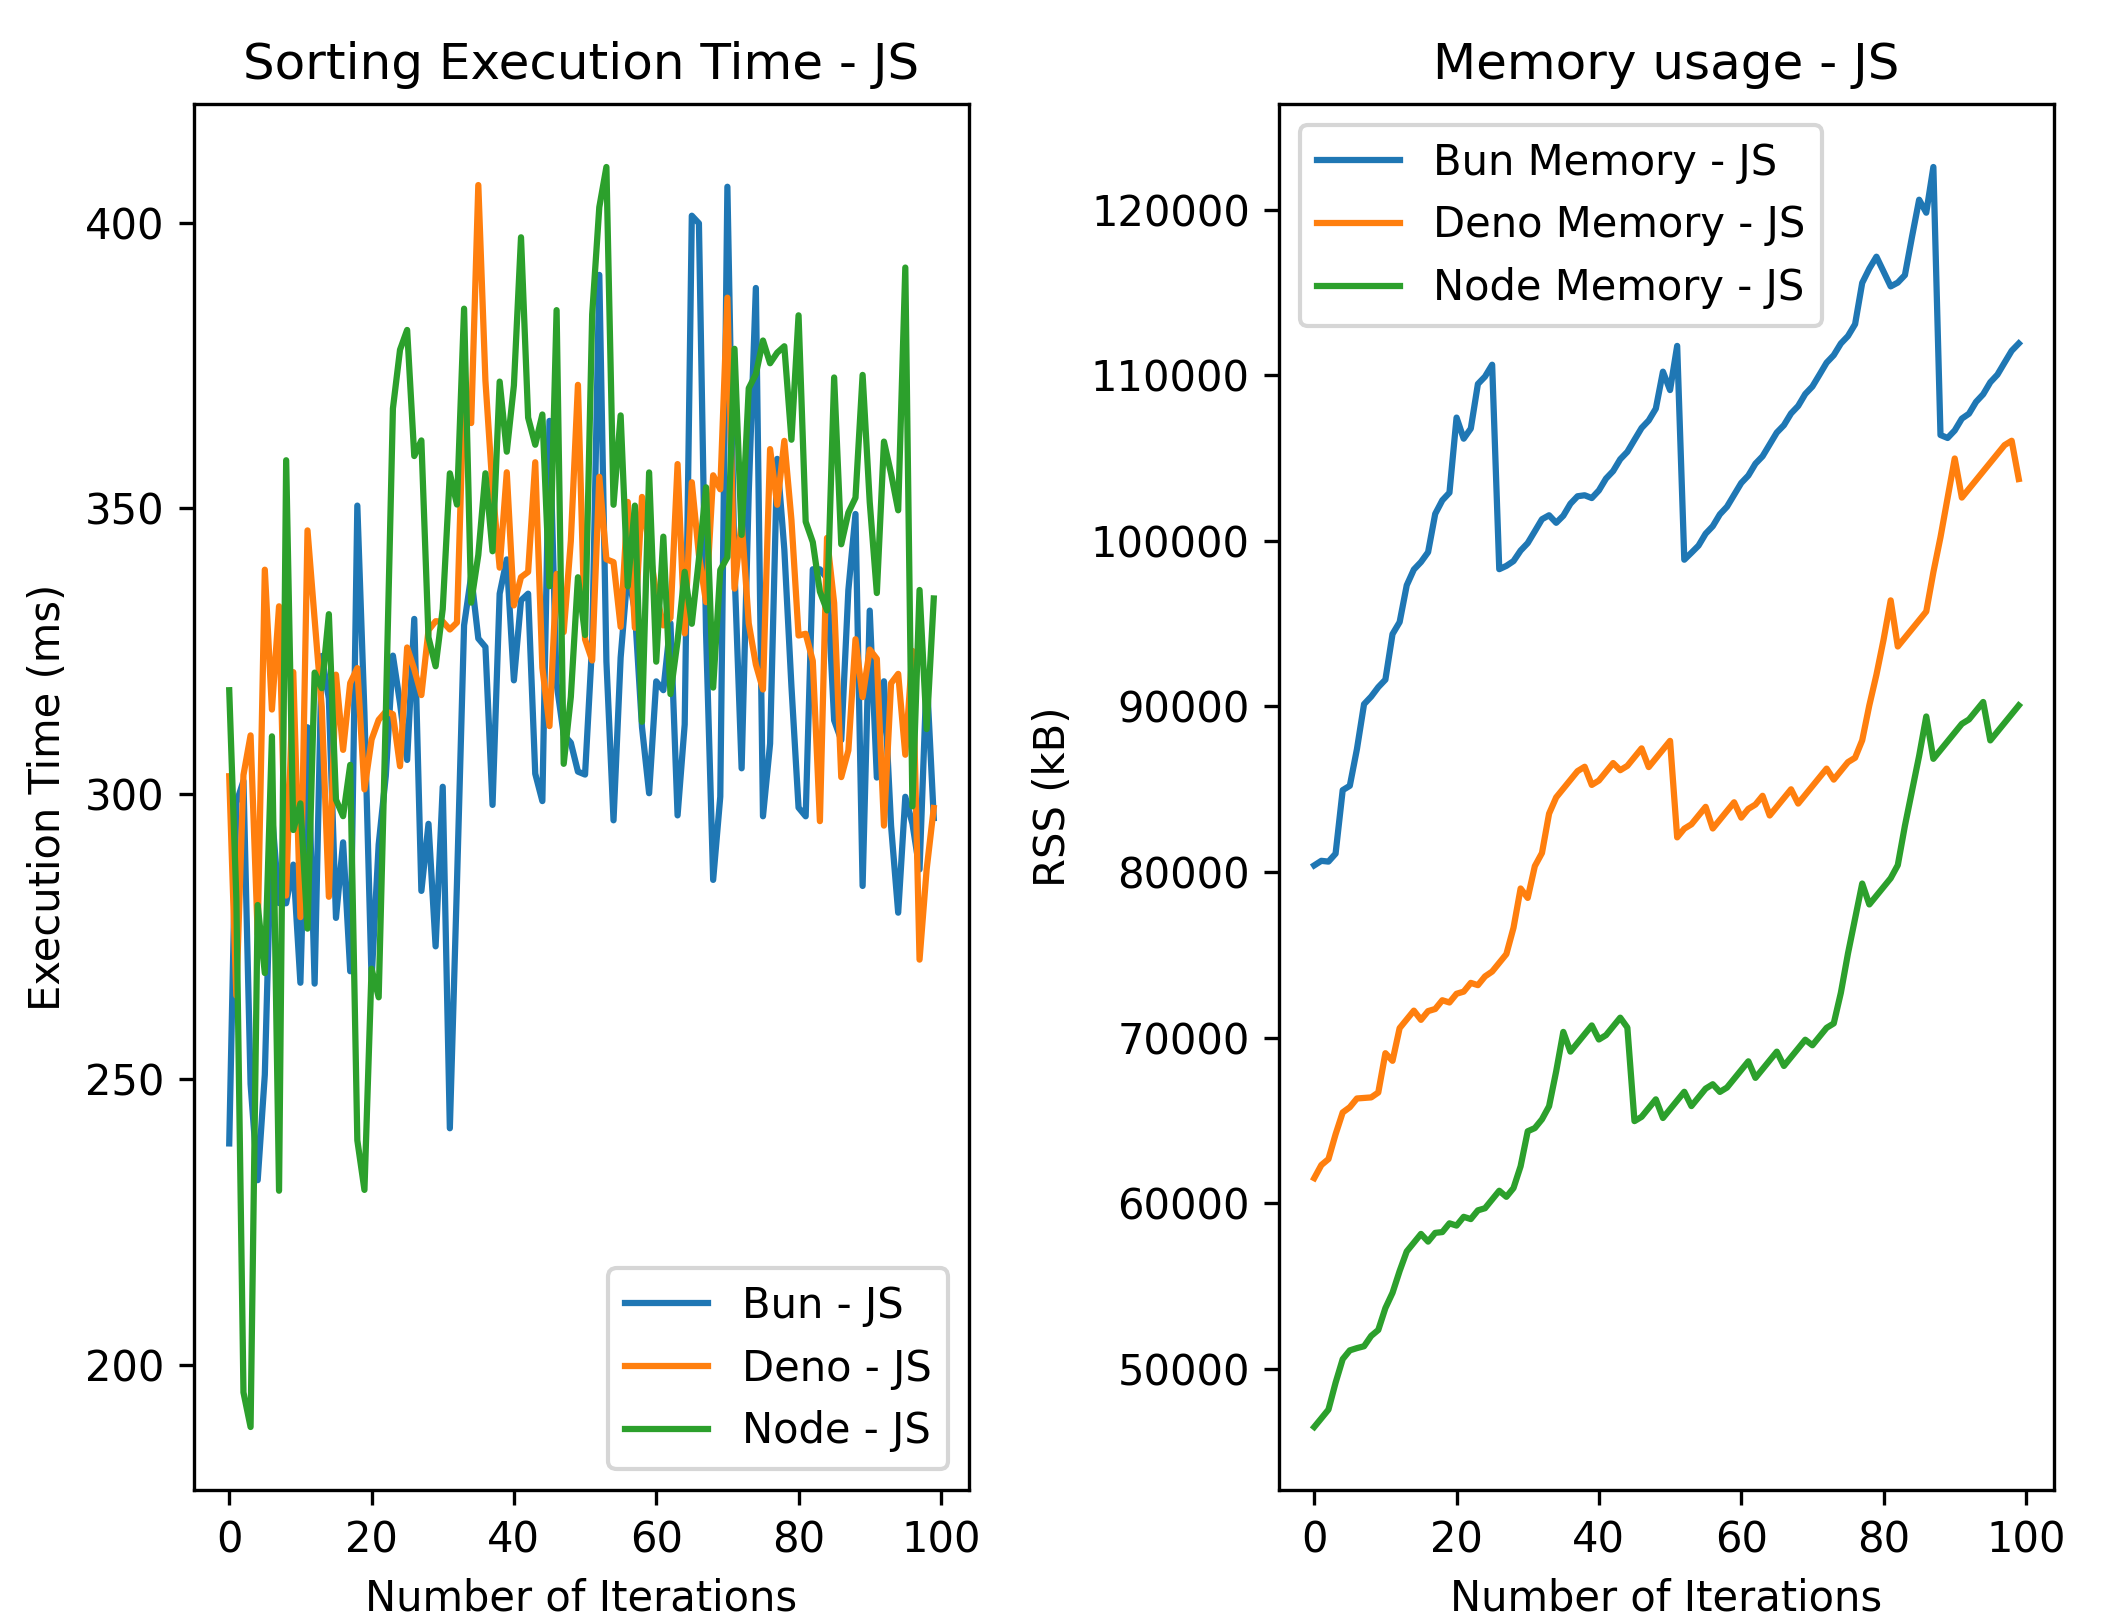
\includegraphics[width=0.7\textwidth]{Figures/sorting/sorting_bubble_100_10000_js.png}
  \caption{Wyniki eksperymentów dla algorytmu sortowania bąbelkowego dla 100 iteracji i 10000 elementów - po lewej czas wykonania jednorazowego testu w milisekundach, po prawej ilość zajmowanej pamięci w kilobajtach (kB)}
  \label{fig:bubble_sorting_e2}
\end{figure}

Na rysunku \ref{fig:bubble_sorting_e2_ts} przedstawiono wyniki eksperymentów dla algorytmu sortowania bąbelkowego dla 100 iteracji i 10000 elementów napisanego w języku TypeScript. Na wykresie przedstawiono czas wykonania jednorazowego testu w milisekundach oraz ilość zajmowanej pamięci w kilobajtach (kB).

\begin{figure}[H]
  \centering
  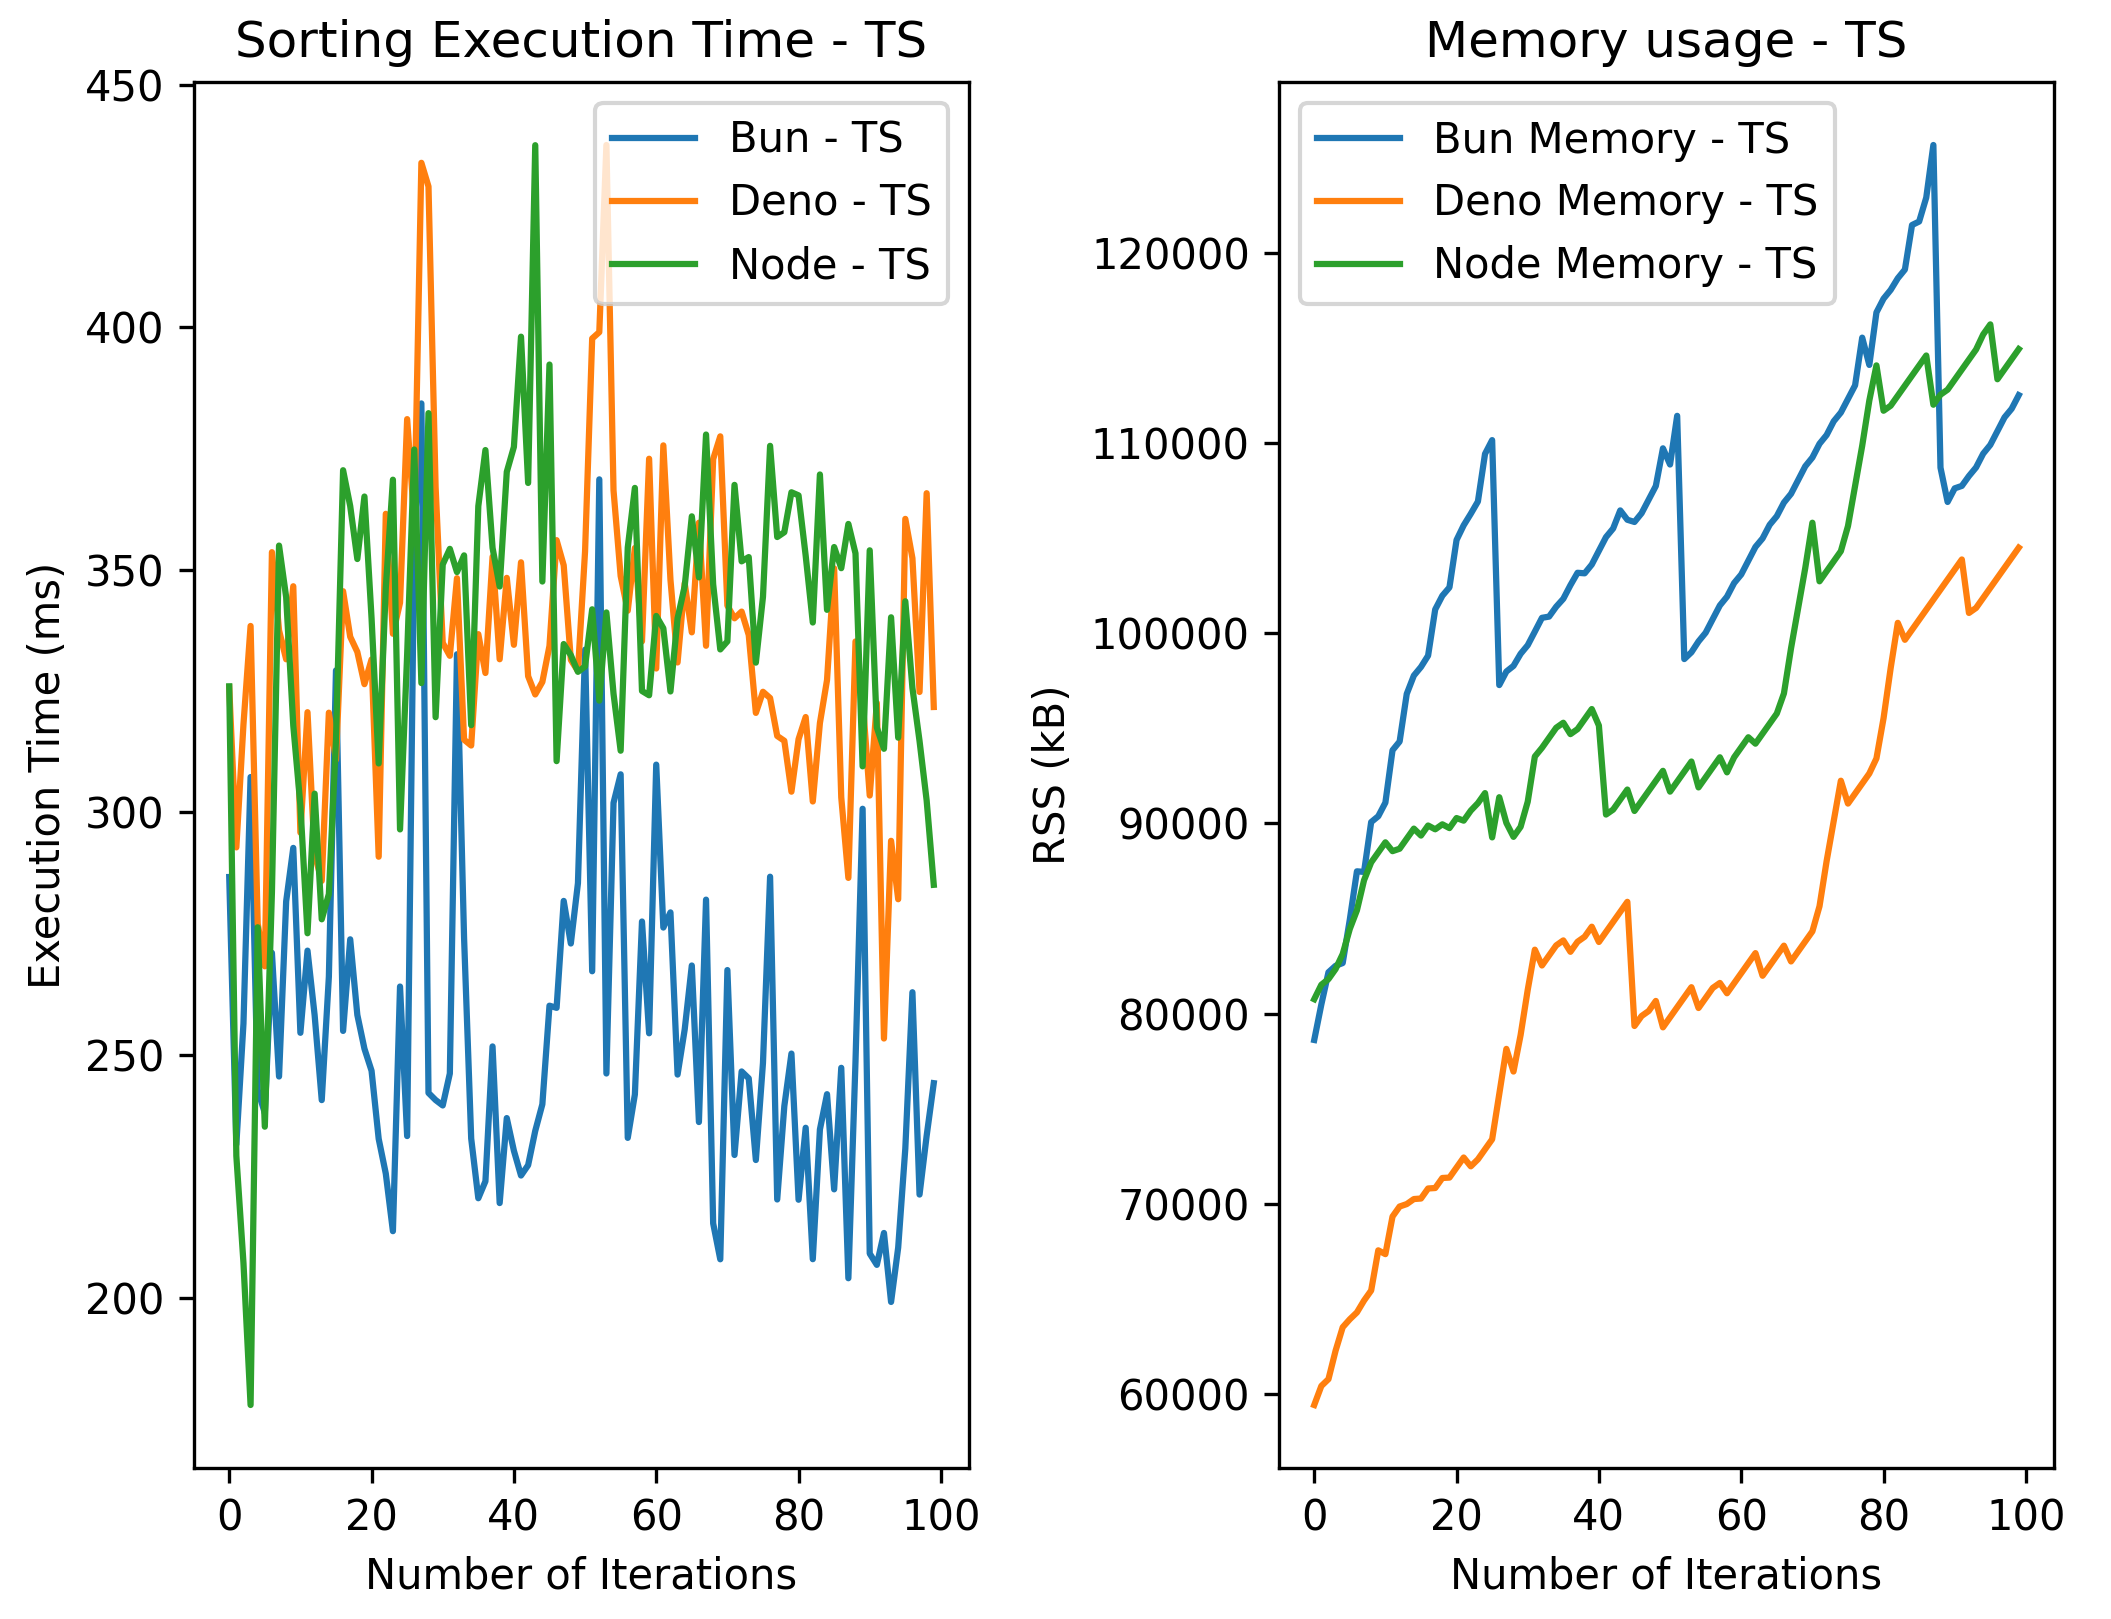
\includegraphics[width=0.7\textwidth]{Figures/sorting/sorting_bubble_100_10000_ts.png}
  \caption{Wyniki eksperymentów dla algorytmu sortowania bąbelkowego dla 100 iteracji i 10000 elementów - po lewej czas wykonania jednorazowego testu w milisekundach, po prawej ilość zajmowanej pamięci w kilobajtach (kB)}
  \label{fig:bubble_sorting_e2_ts}
\end{figure}

Na rysunku \ref{fig:bubble_sorting_e3} przedstawiono wyniki eksperymentów dla algorytmu sortowania bąbelkowego dla 1000 iteracji i 1000 elementów napisanego w języku JavaScript. Na wykresie przedstawiono czas wykonania jednorazowego testu w milisekundach oraz ilość zajmowanej pamięci w kilobajtach (kB).

\begin{figure}[H]
  \centering
  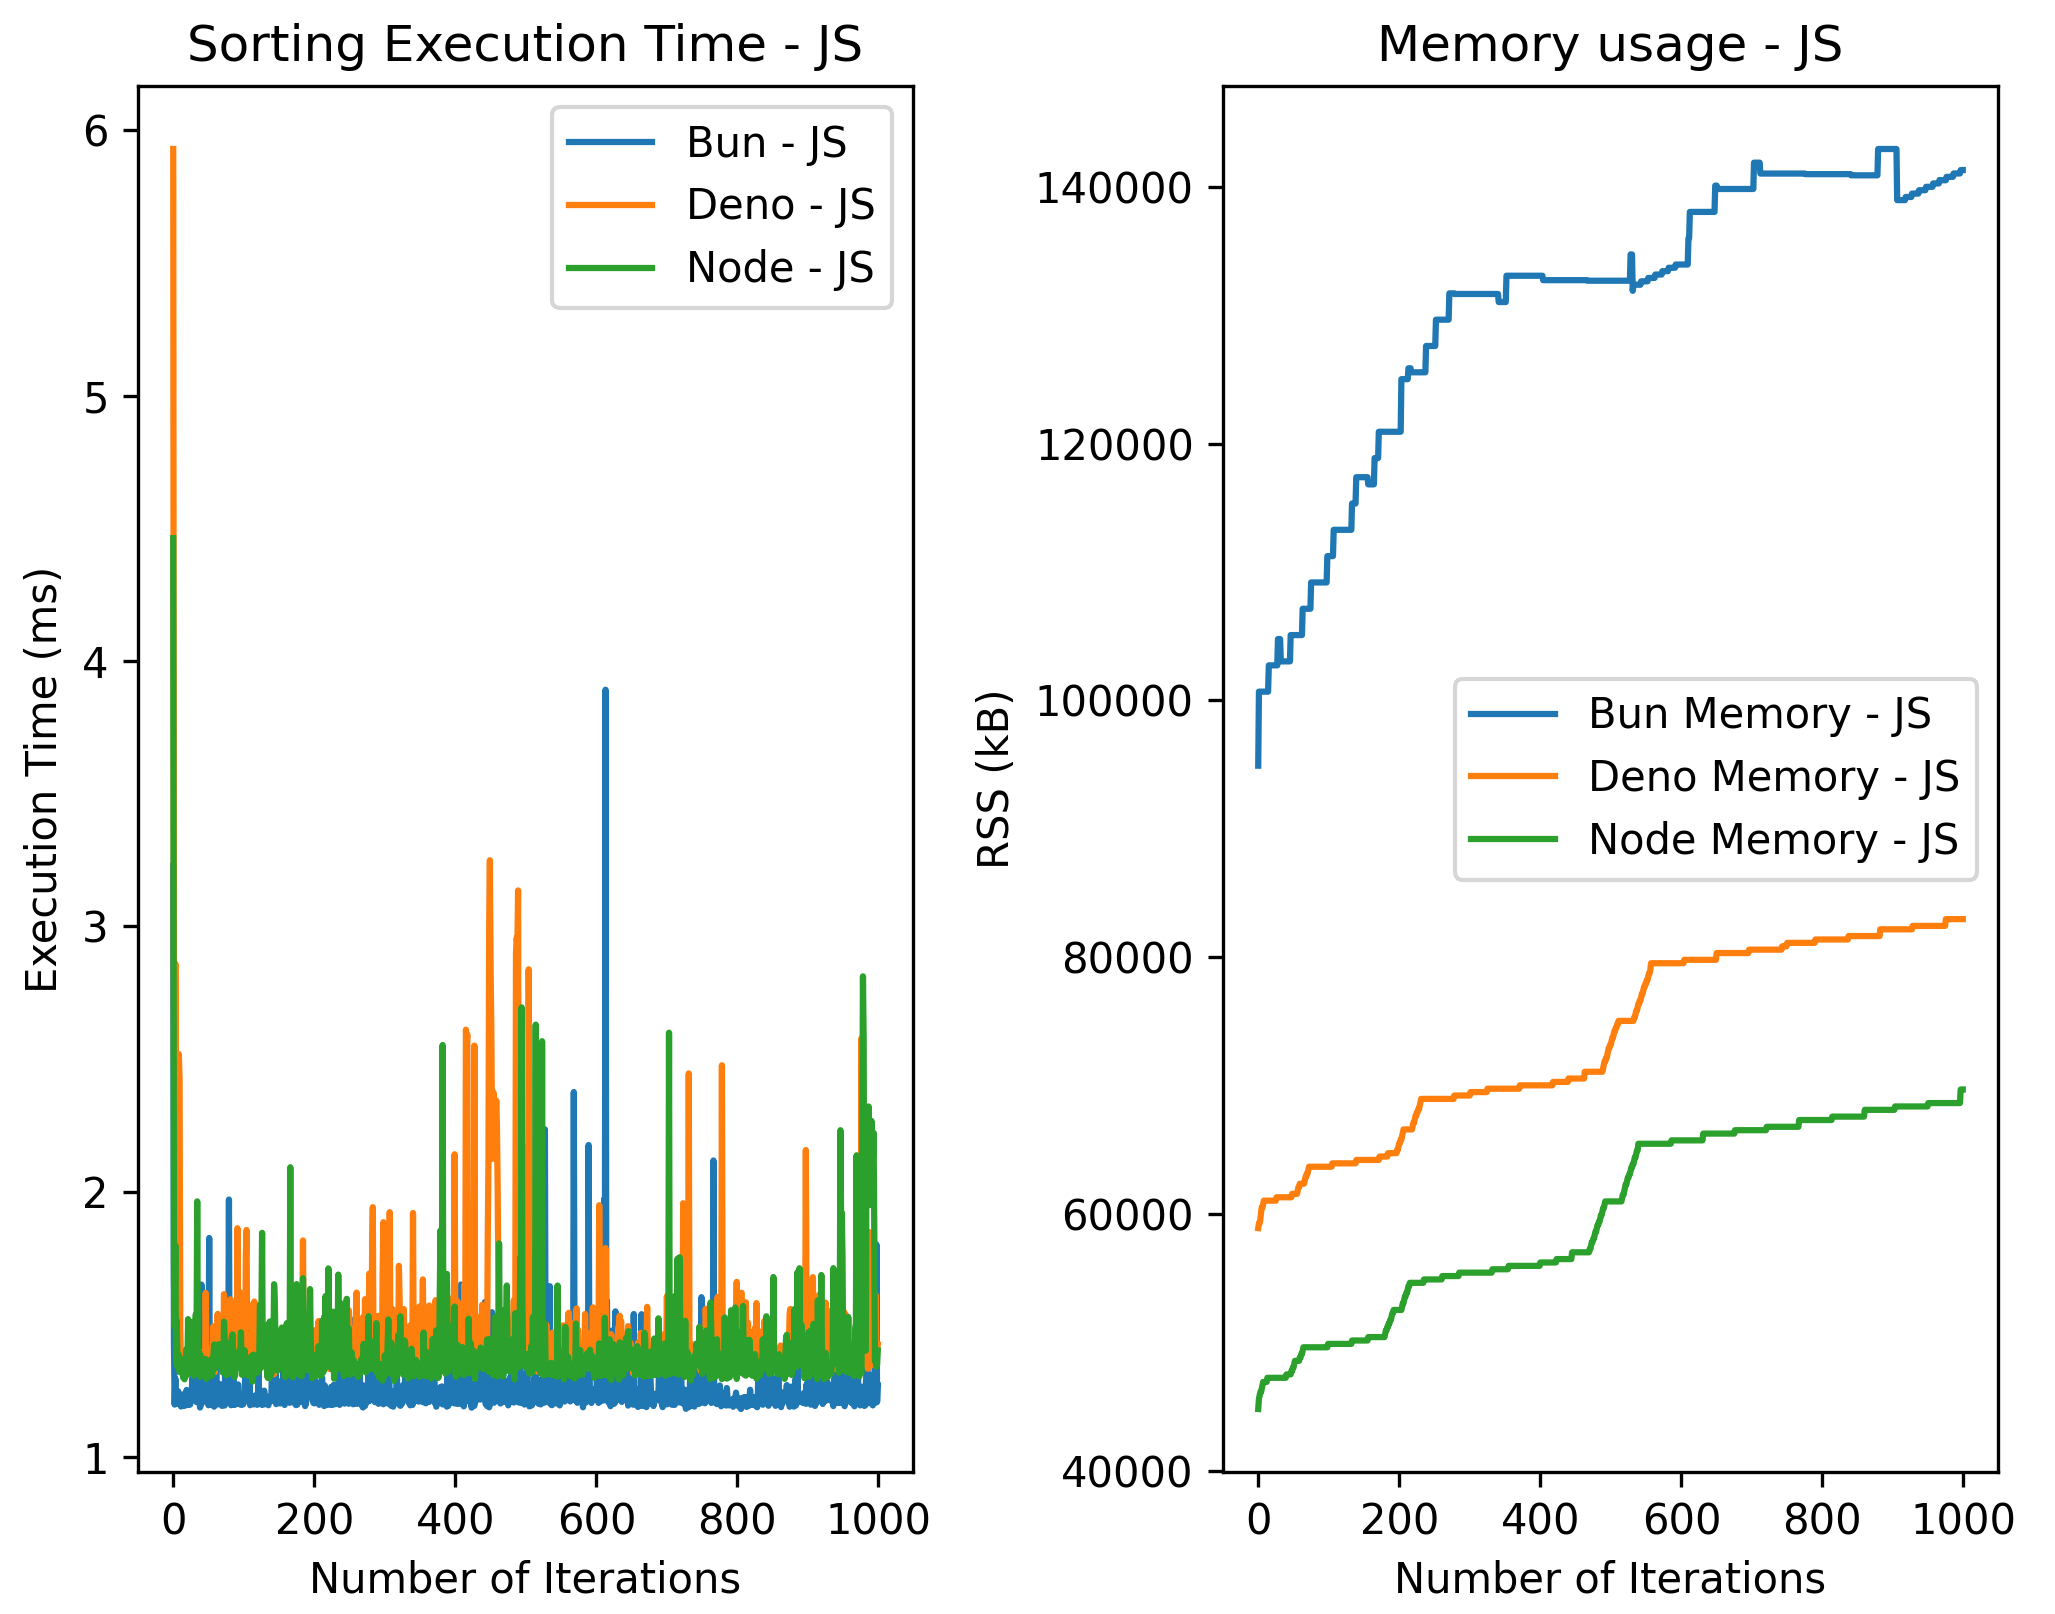
\includegraphics[width=0.7\textwidth]{Figures/sorting/sorting_bubble_1000_1000_js.png}
  \caption{Wyniki eksperymentów dla algorytmu sortowania bąbelkowego dla 1000 iteracji i 1000 elementów - po lewej czas wykonania jednorazowego testu w milisekundach, po prawej ilość zajmowanej pamięci w kilobajtach (kB)}
  \label{fig:bubble_sorting_e3}
\end{figure}

Na rysunku \ref{fig:bubble_sorting_e3_ts} przedstawiono wyniki eksperymentów dla algorytmu sortowania bąbelkowego dla 1000 iteracji i 1000 elementów napisanego w języku TypeScript. Na wykresie przedstawiono czas wykonania jednorazowego testu w milisekundach oraz ilość zajmowanej pamięci w kilobajtach (kB).

\begin{figure}[H]
  \centering
  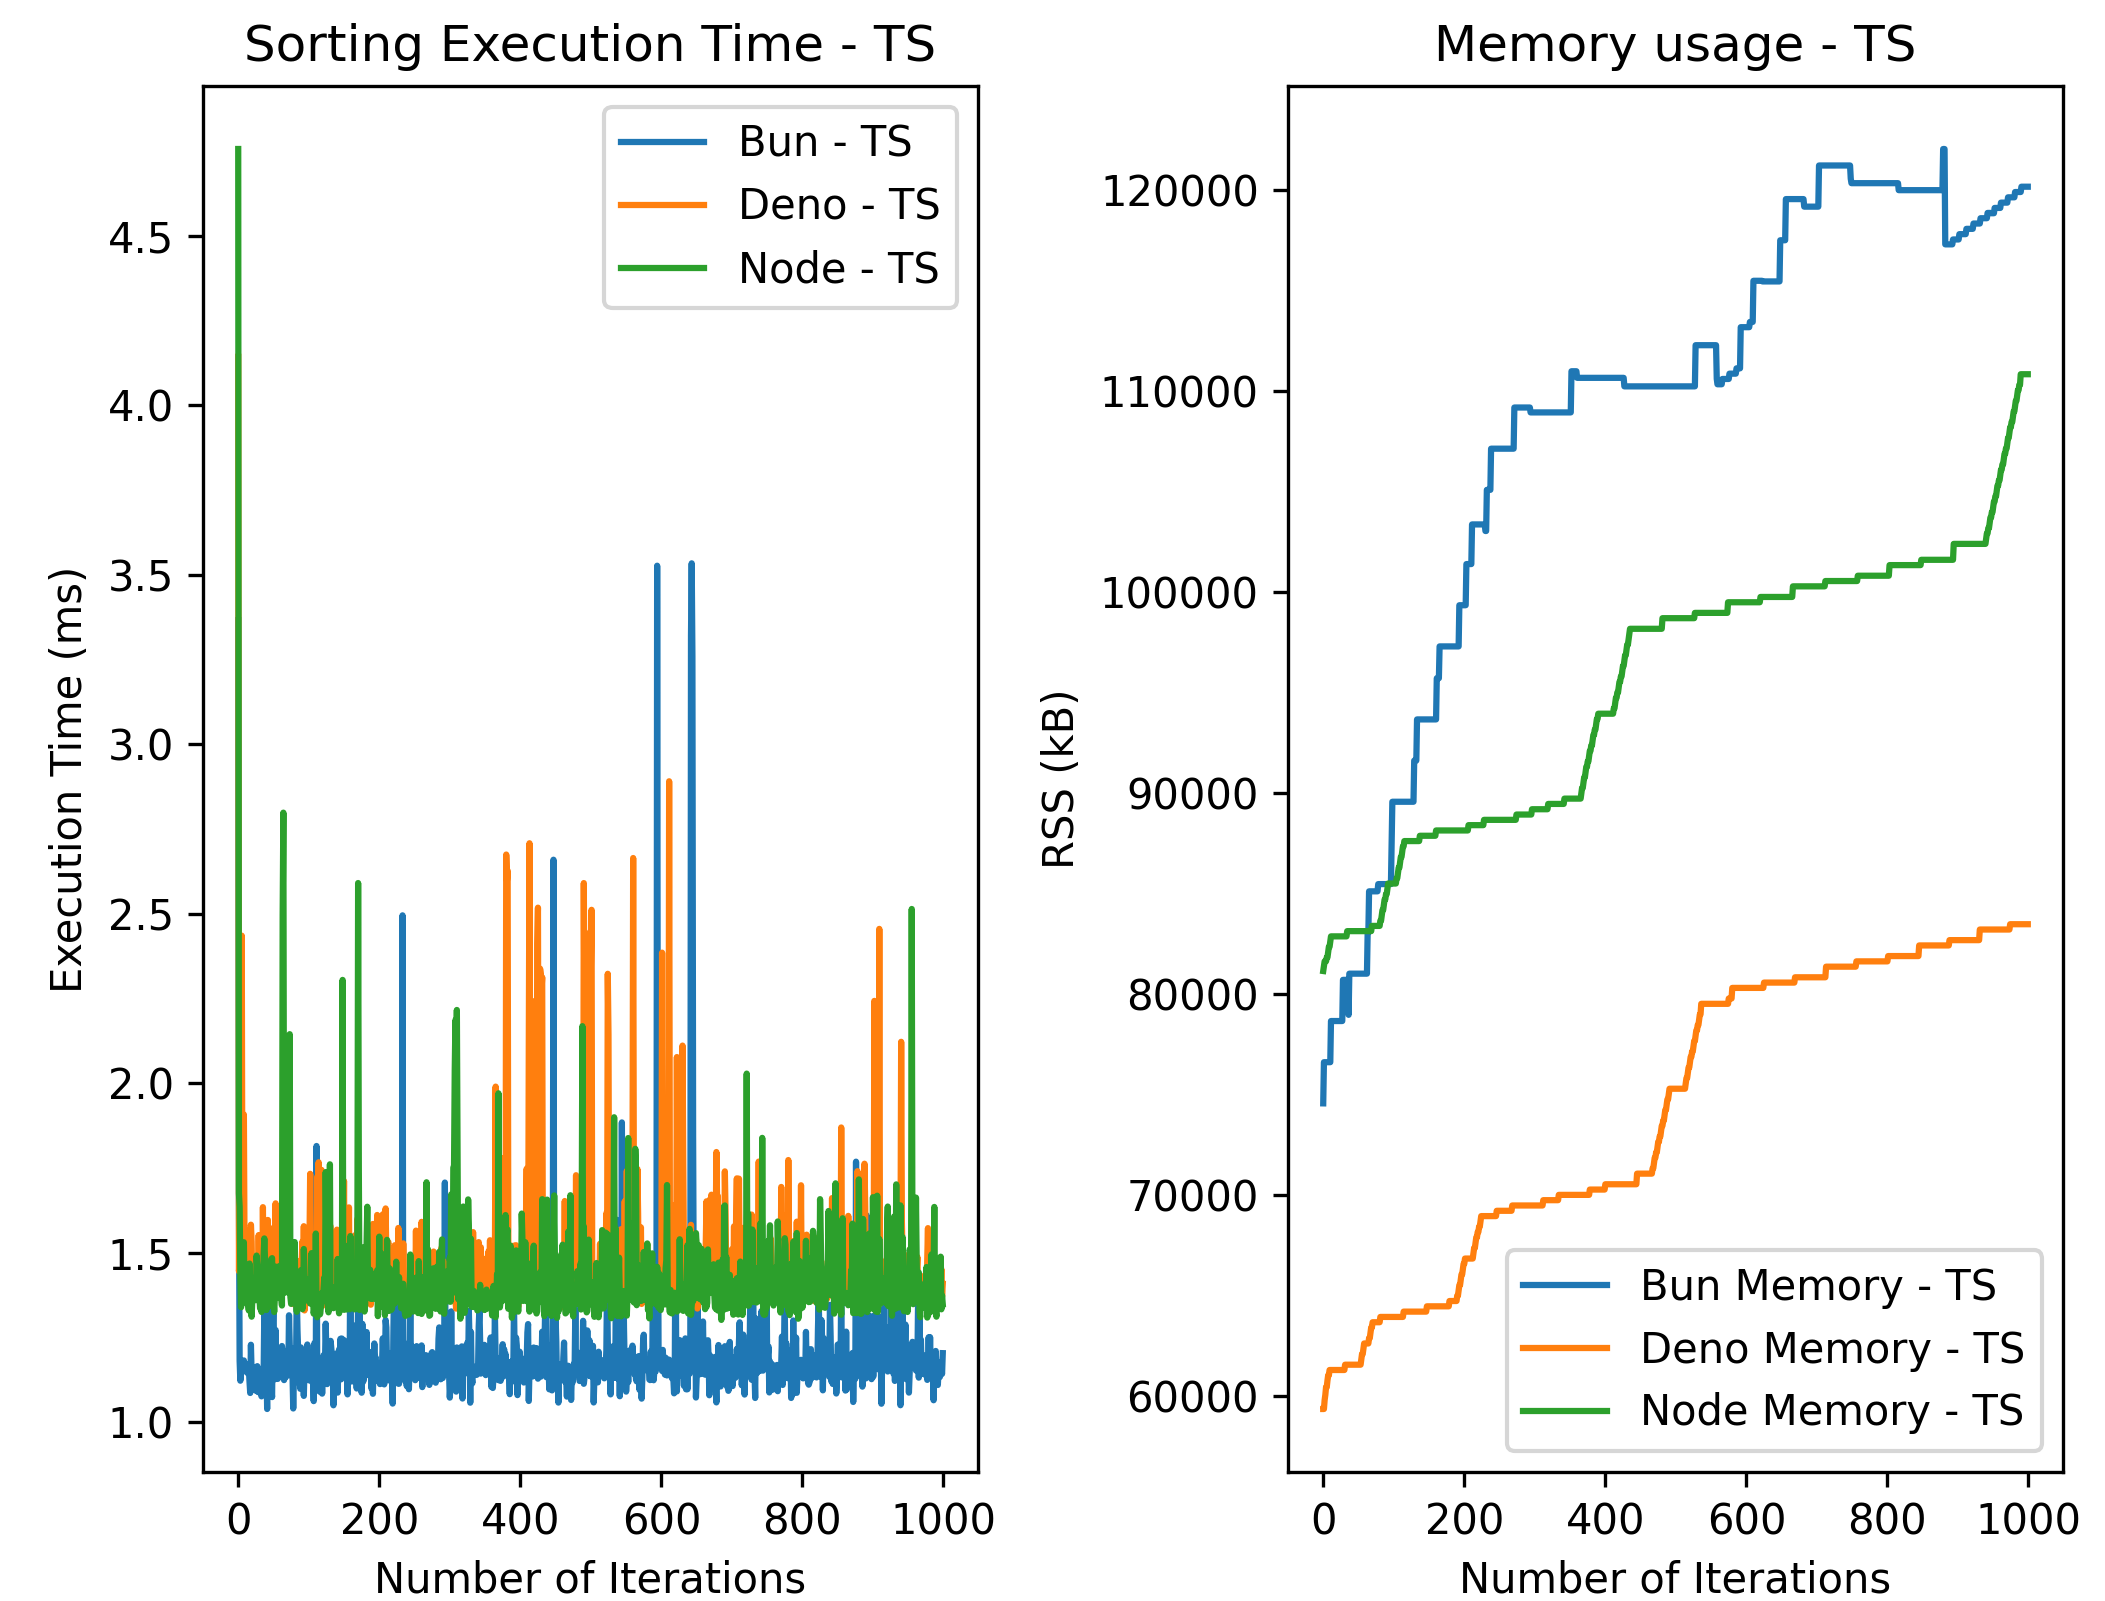
\includegraphics[width=0.7\textwidth]{Figures/sorting/sorting_bubble_1000_1000_ts.png}
  \caption{Wyniki eksperymentów dla algorytmu sortowania bąbelkowego dla 100 iteracji i 1000 elementów - po lewej czas wykonania jednorazowego testu w milisekundach, po prawej ilość zajmowanej pamięci w kilobajtach (kB)}
  \label{fig:bubble_sorting_e3_ts}
\end{figure}

Na rysunku \ref{fig:bubble_sorting_e4} przedstawiono wyniki eksperymentów dla algorytmu sortowania bąbelkowego dla 100 iteracji i 1000 elementów napisanego w języku JavaScript. Na wykresie przedstawiono czas wykonania jednorazowego testu w milisekundach oraz ilość zajmowanej pamięci w kilobajtach (kB).

\begin{figure}[H]
  \centering
  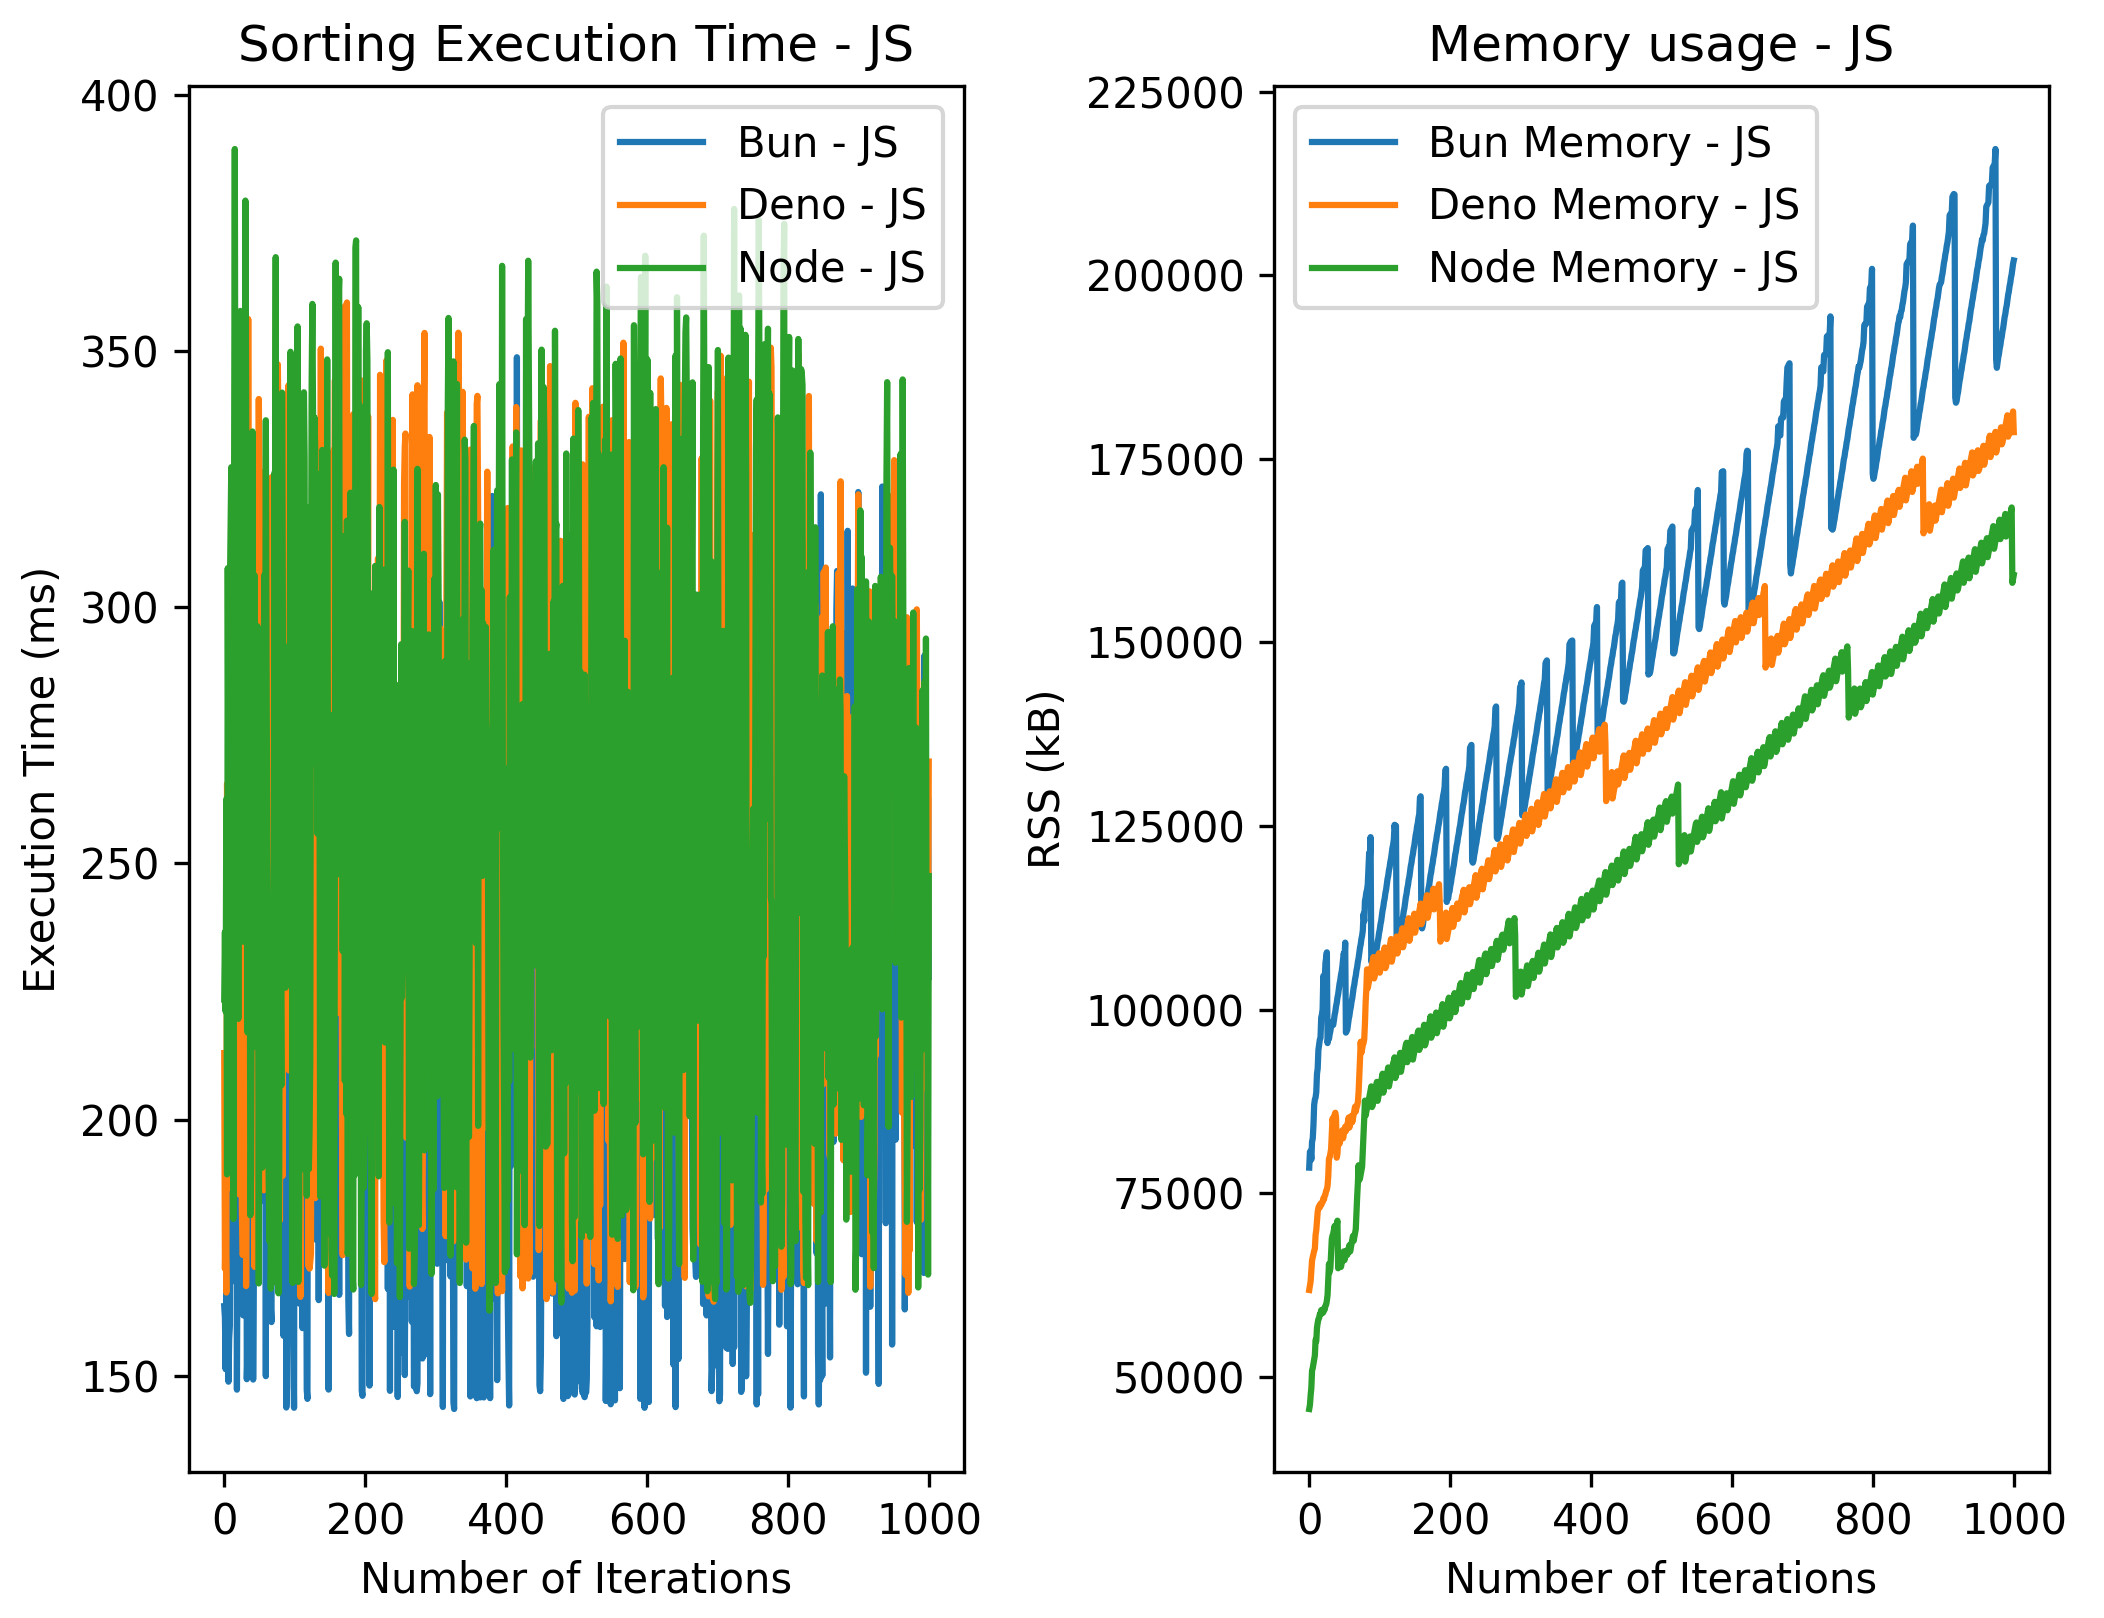
\includegraphics[width=0.7\textwidth]{Figures/sorting/sorting_bubble_1000_10000_js.png}
  \caption{Wyniki eksperymentów dla algorytmu sortowania bąbelkowego dla 100 iteracji i 10000 elementów - po lewej czas wykonania jednorazowego testu w milisekundach, po prawej ilość zajmowanej pamięci w kilobajtach (kB)}
  \label{fig:bubble_sorting_e4}
\end{figure}

Na rysunku \ref{fig:bubble_sorting_e4_ts} przedstawiono wyniki eksperymentów dla algorytmu sortowania bąbelkowego dla 100 iteracji i 10000 elementów napisanego w języku TypeScript. Na wykresie przedstawiono czas wykonania jednorazowego testu w milisekundach oraz ilość zajmowanej pamięci w kilobajtach (kB).

\begin{figure}[H]
  \centering
  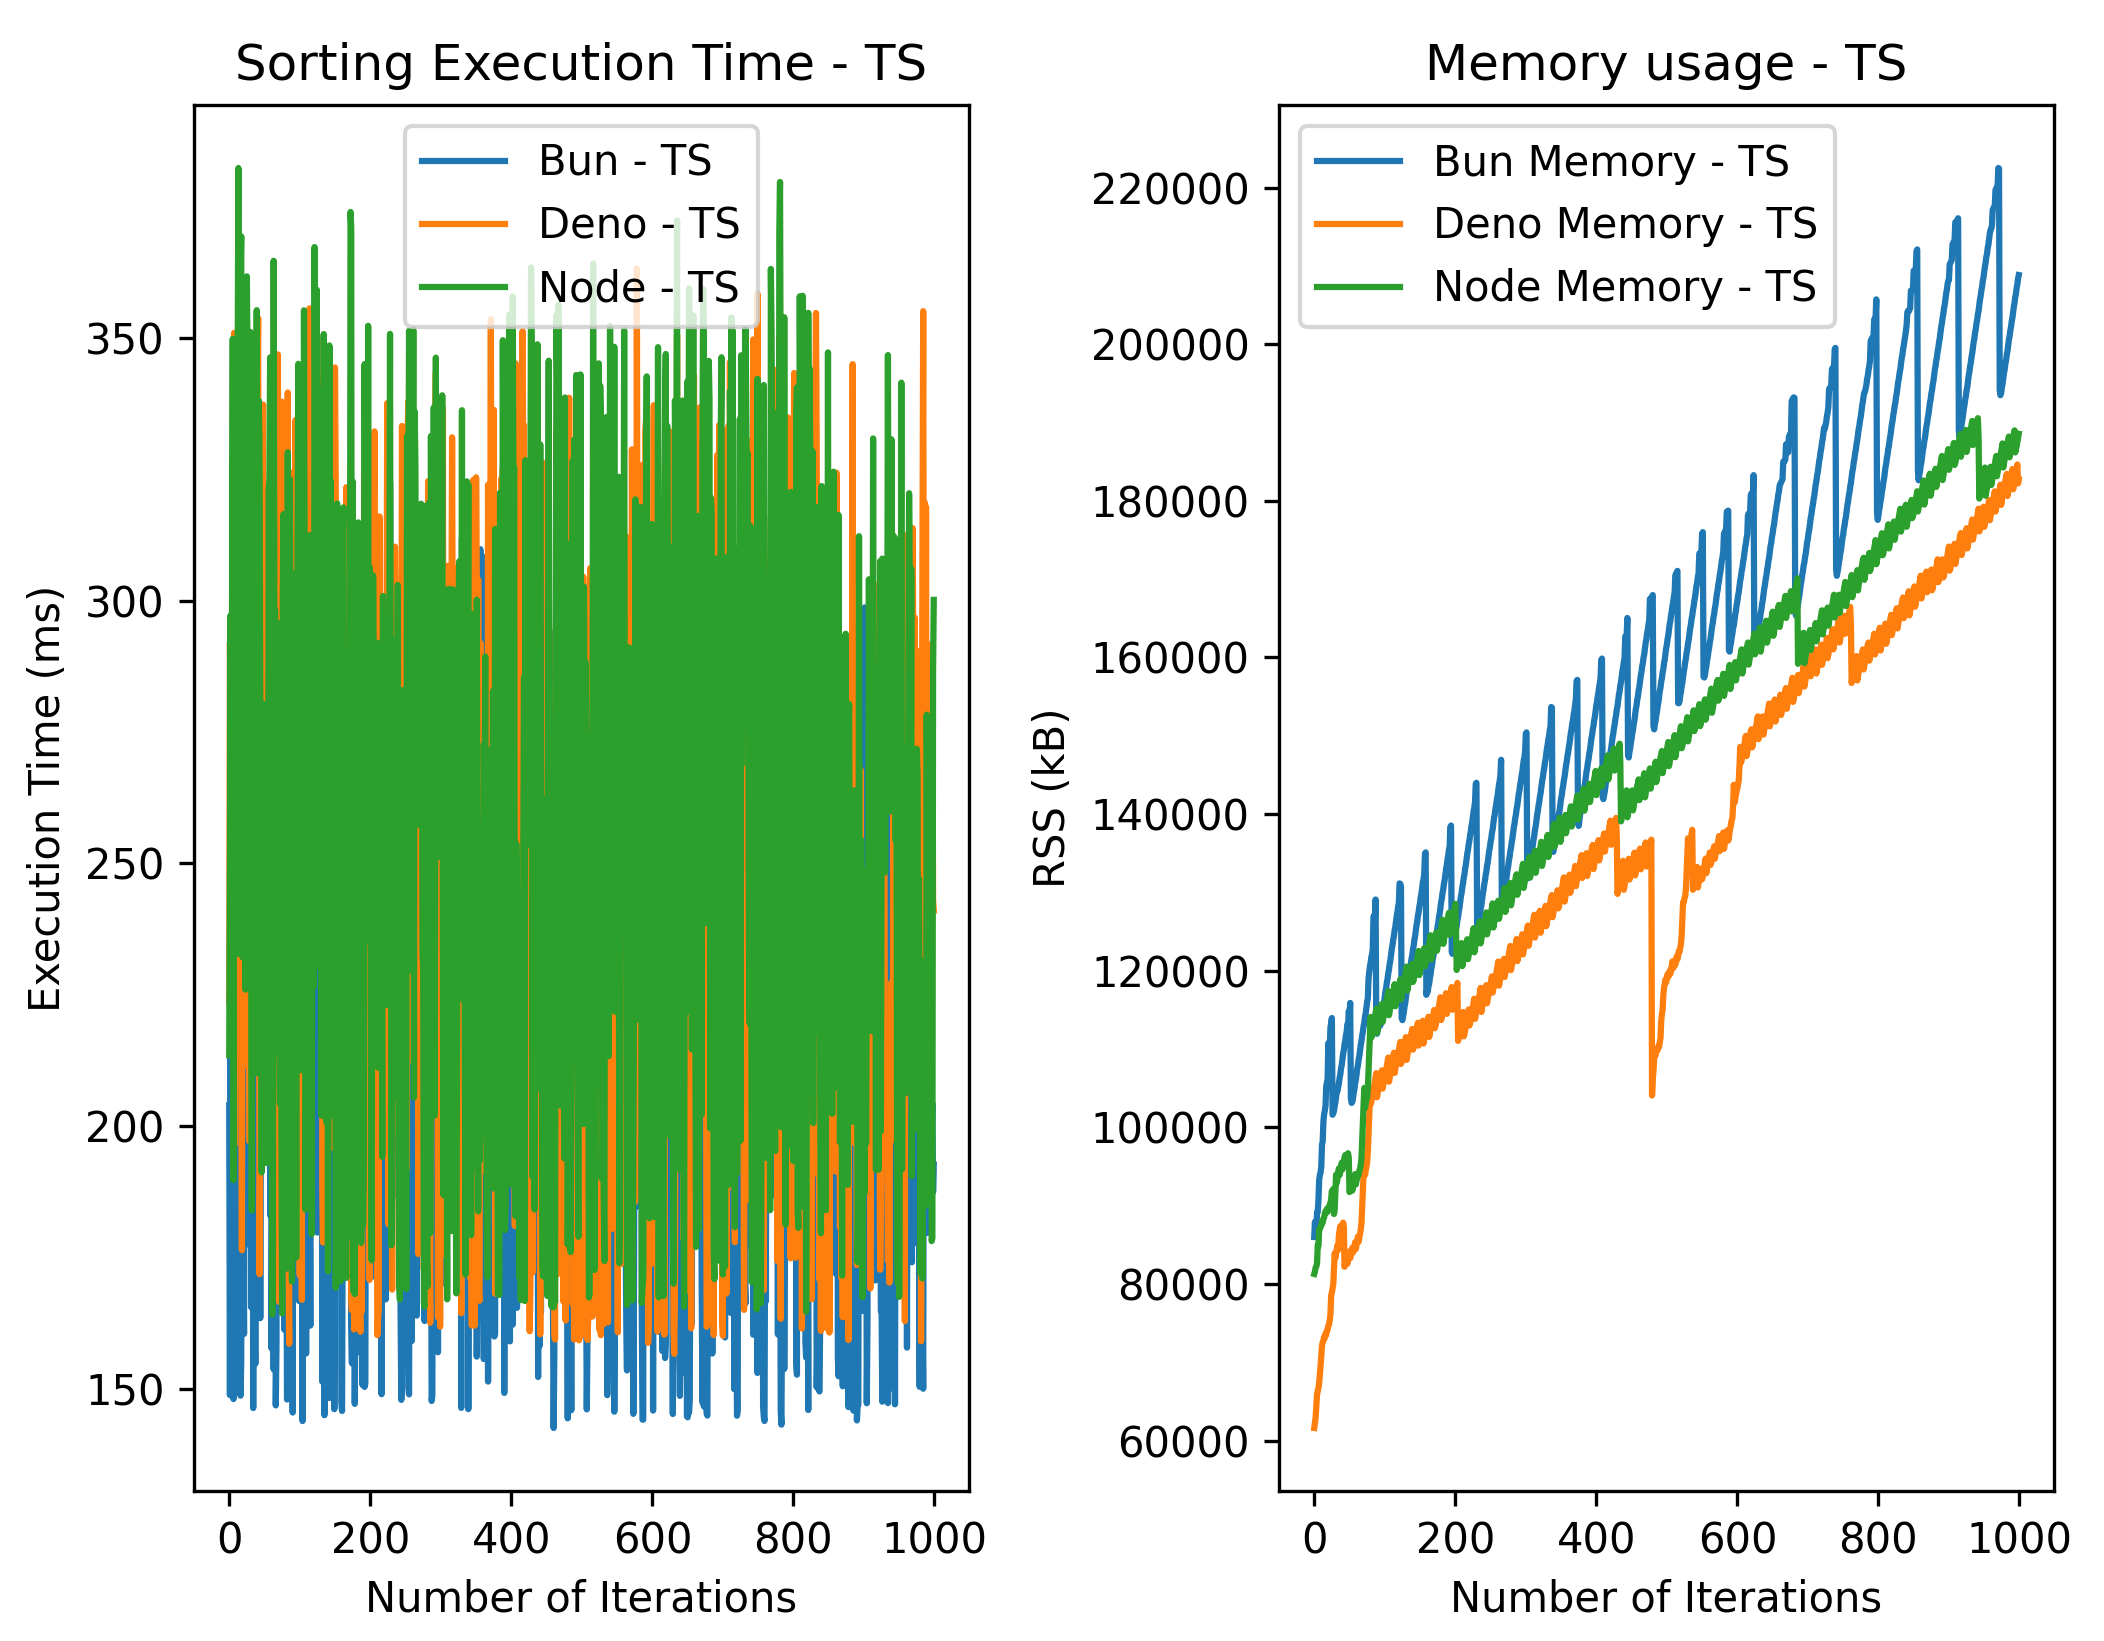
\includegraphics[width=0.7\textwidth]{Figures/sorting/sorting_bubble_1000_10000_ts.png}
  \caption{Wyniki eksperymentów dla algorytmu sortowania bąbelkowego dla 1000 iteracji i 10000 elementów - po lewej czas wykonania jednorazowego testu w milisekundach, po prawej ilość zajmowanej pamięci w kilobajtach (kB)}
  \label{fig:bubble_sorting_e4_ts}
\end{figure}

\subsubsection{Wyniki - sortowanie szybkie}
Na rysunku \ref{fig:quick_sorting_e1} przedstawiono wyniki eksperymentów dla algorytmu sortowania szybkiego dla 100 iteracji i 1000 elementów napisanego w języku JavaScript. Na wykresie przedstawiono czas wykonania jednorazowego testu w milisekundach oraz ilość zajmowanej pamięci w kilobajtach (kB).

\begin{figure}[H]
  \centering
  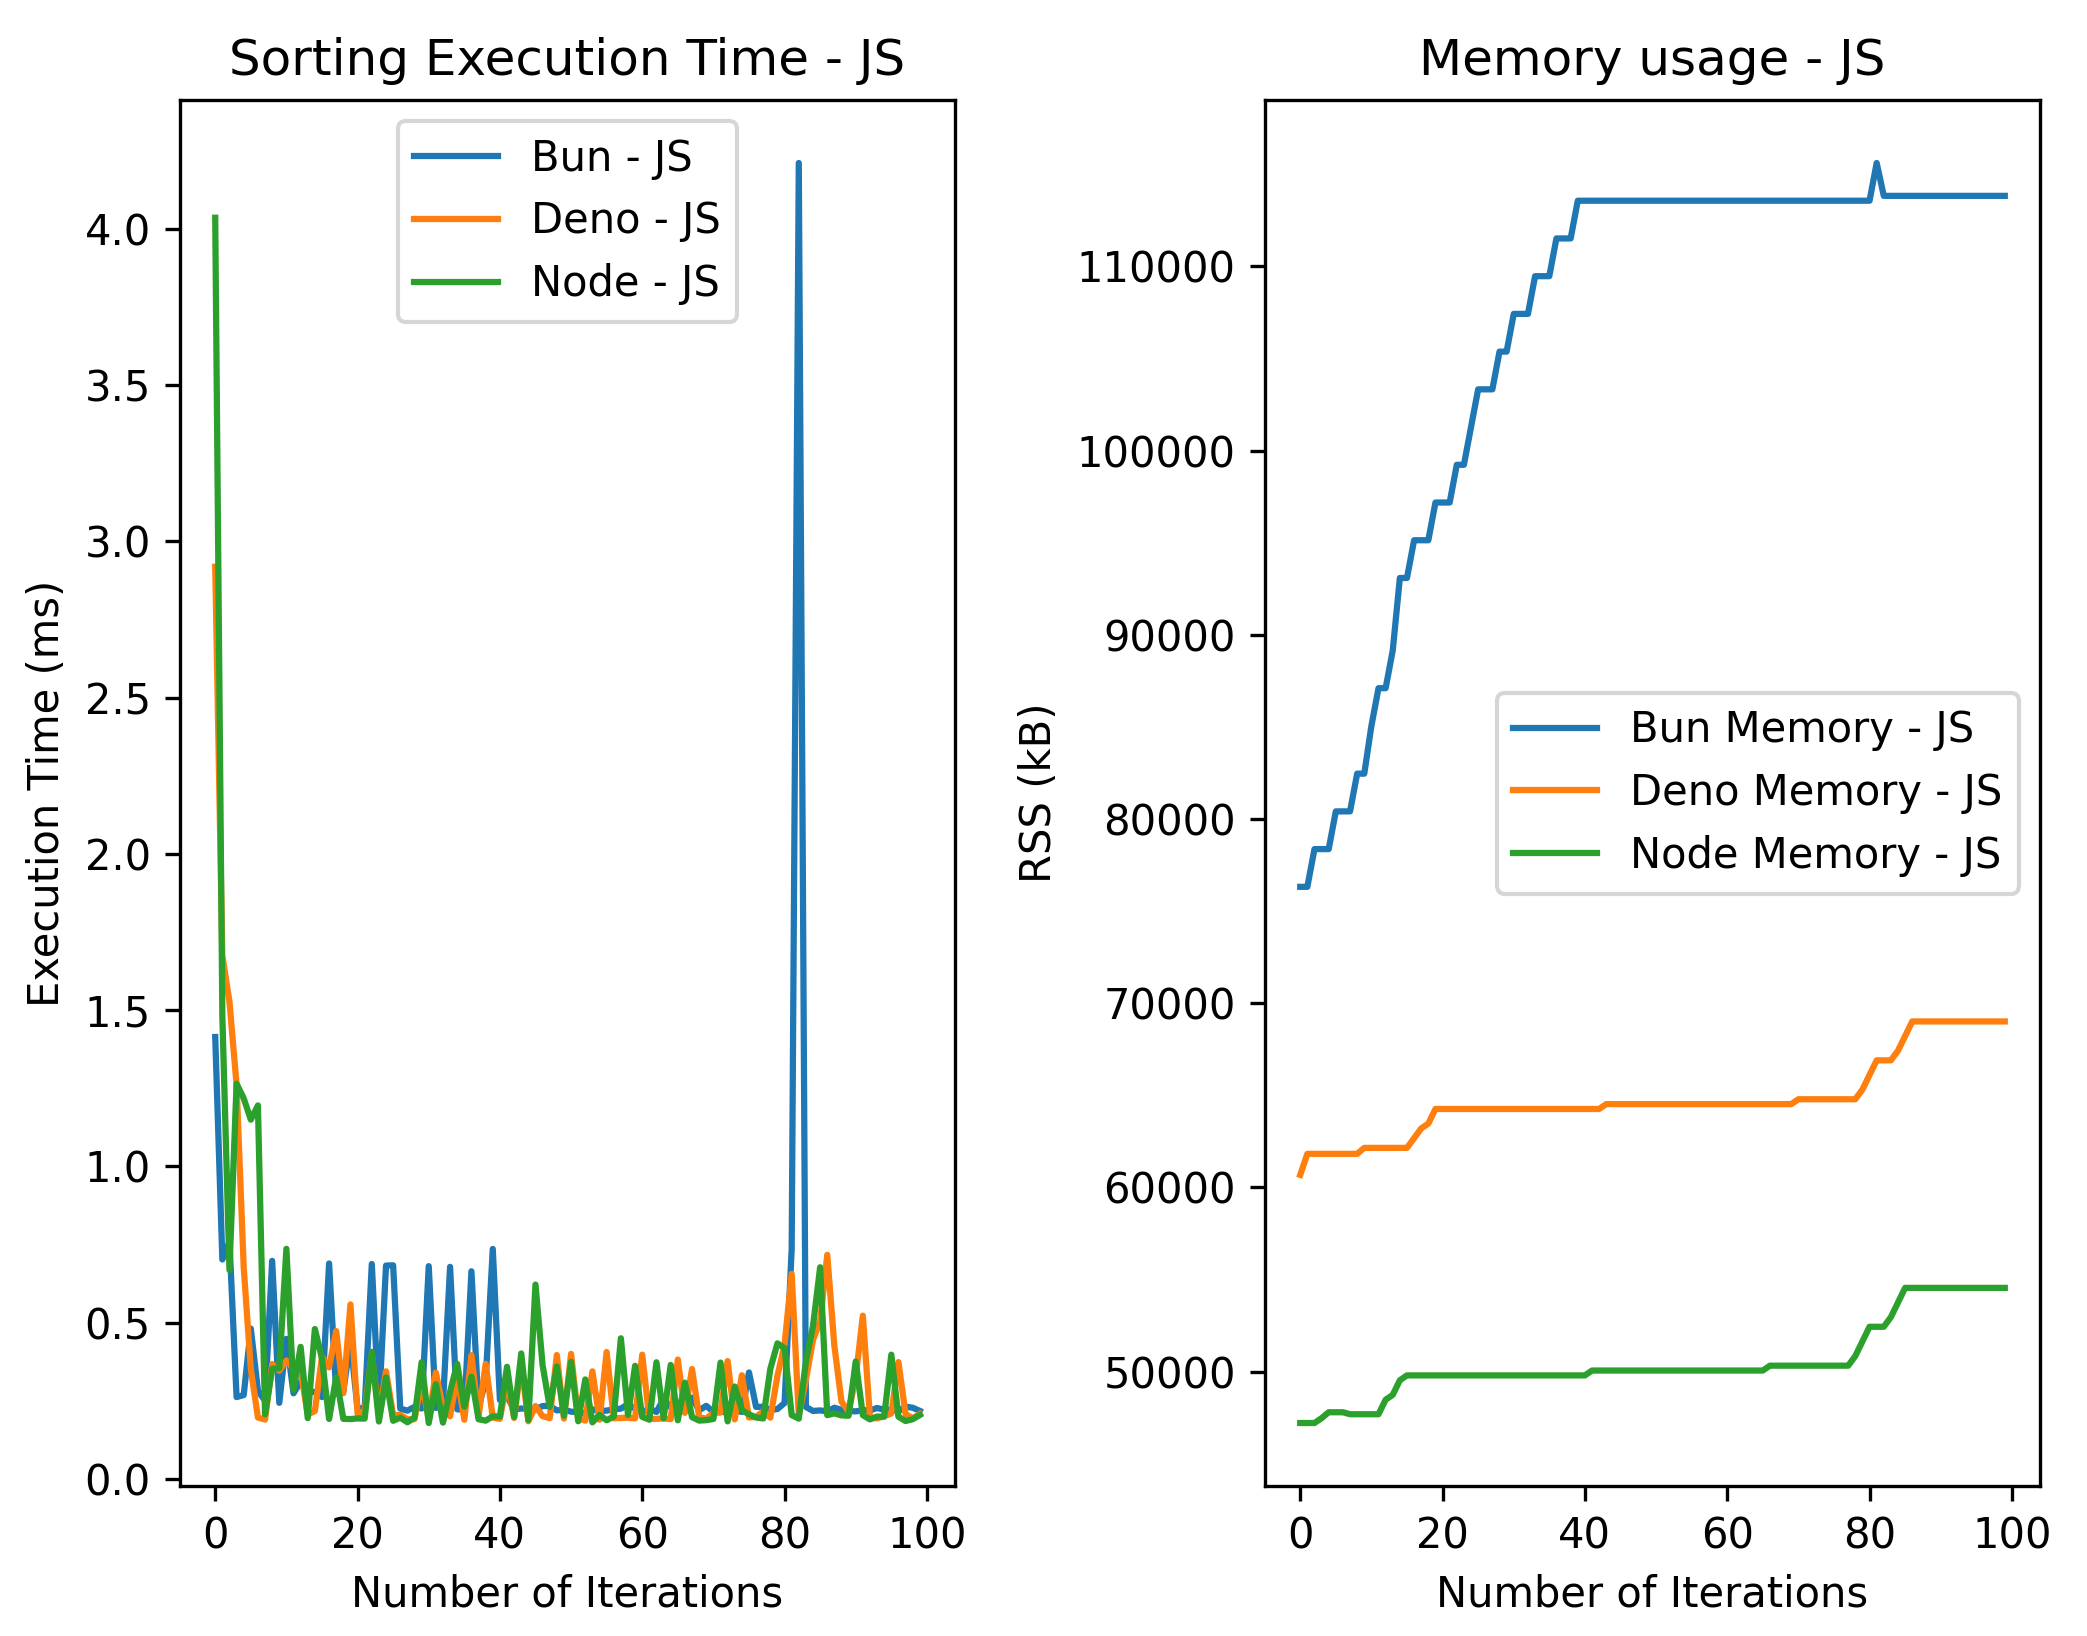
\includegraphics[width=0.7\textwidth]{Figures/sorting/sorting_quick_100_1000_js.png}
  \caption{Wyniki eksperymentów dla algorytmu sortowania szybkiego dla 100 iteracji i 1000 elementów - po lewej czas wykonania jednorazowego testu w milisekundach, po prawej ilość zajmowanej pamięci w kilobajtach (kB)}
  \label{fig:quick_sorting_e1}
\end{figure}

Na rysunku \ref{fig:quick_sorting_e1_ts} przedstawiono wyniki eksperymentów dla algorytmu sortowania szybkiego dla 100 iteracji i 1000 elementów napisanego w języku TypeScript. Na wykresie przedstawiono czas wykonania jednorazowego testu w milisekundach oraz ilość zajmowanej pamięci w kilobajtach (kB).

\begin{figure}[H]
  \centering
  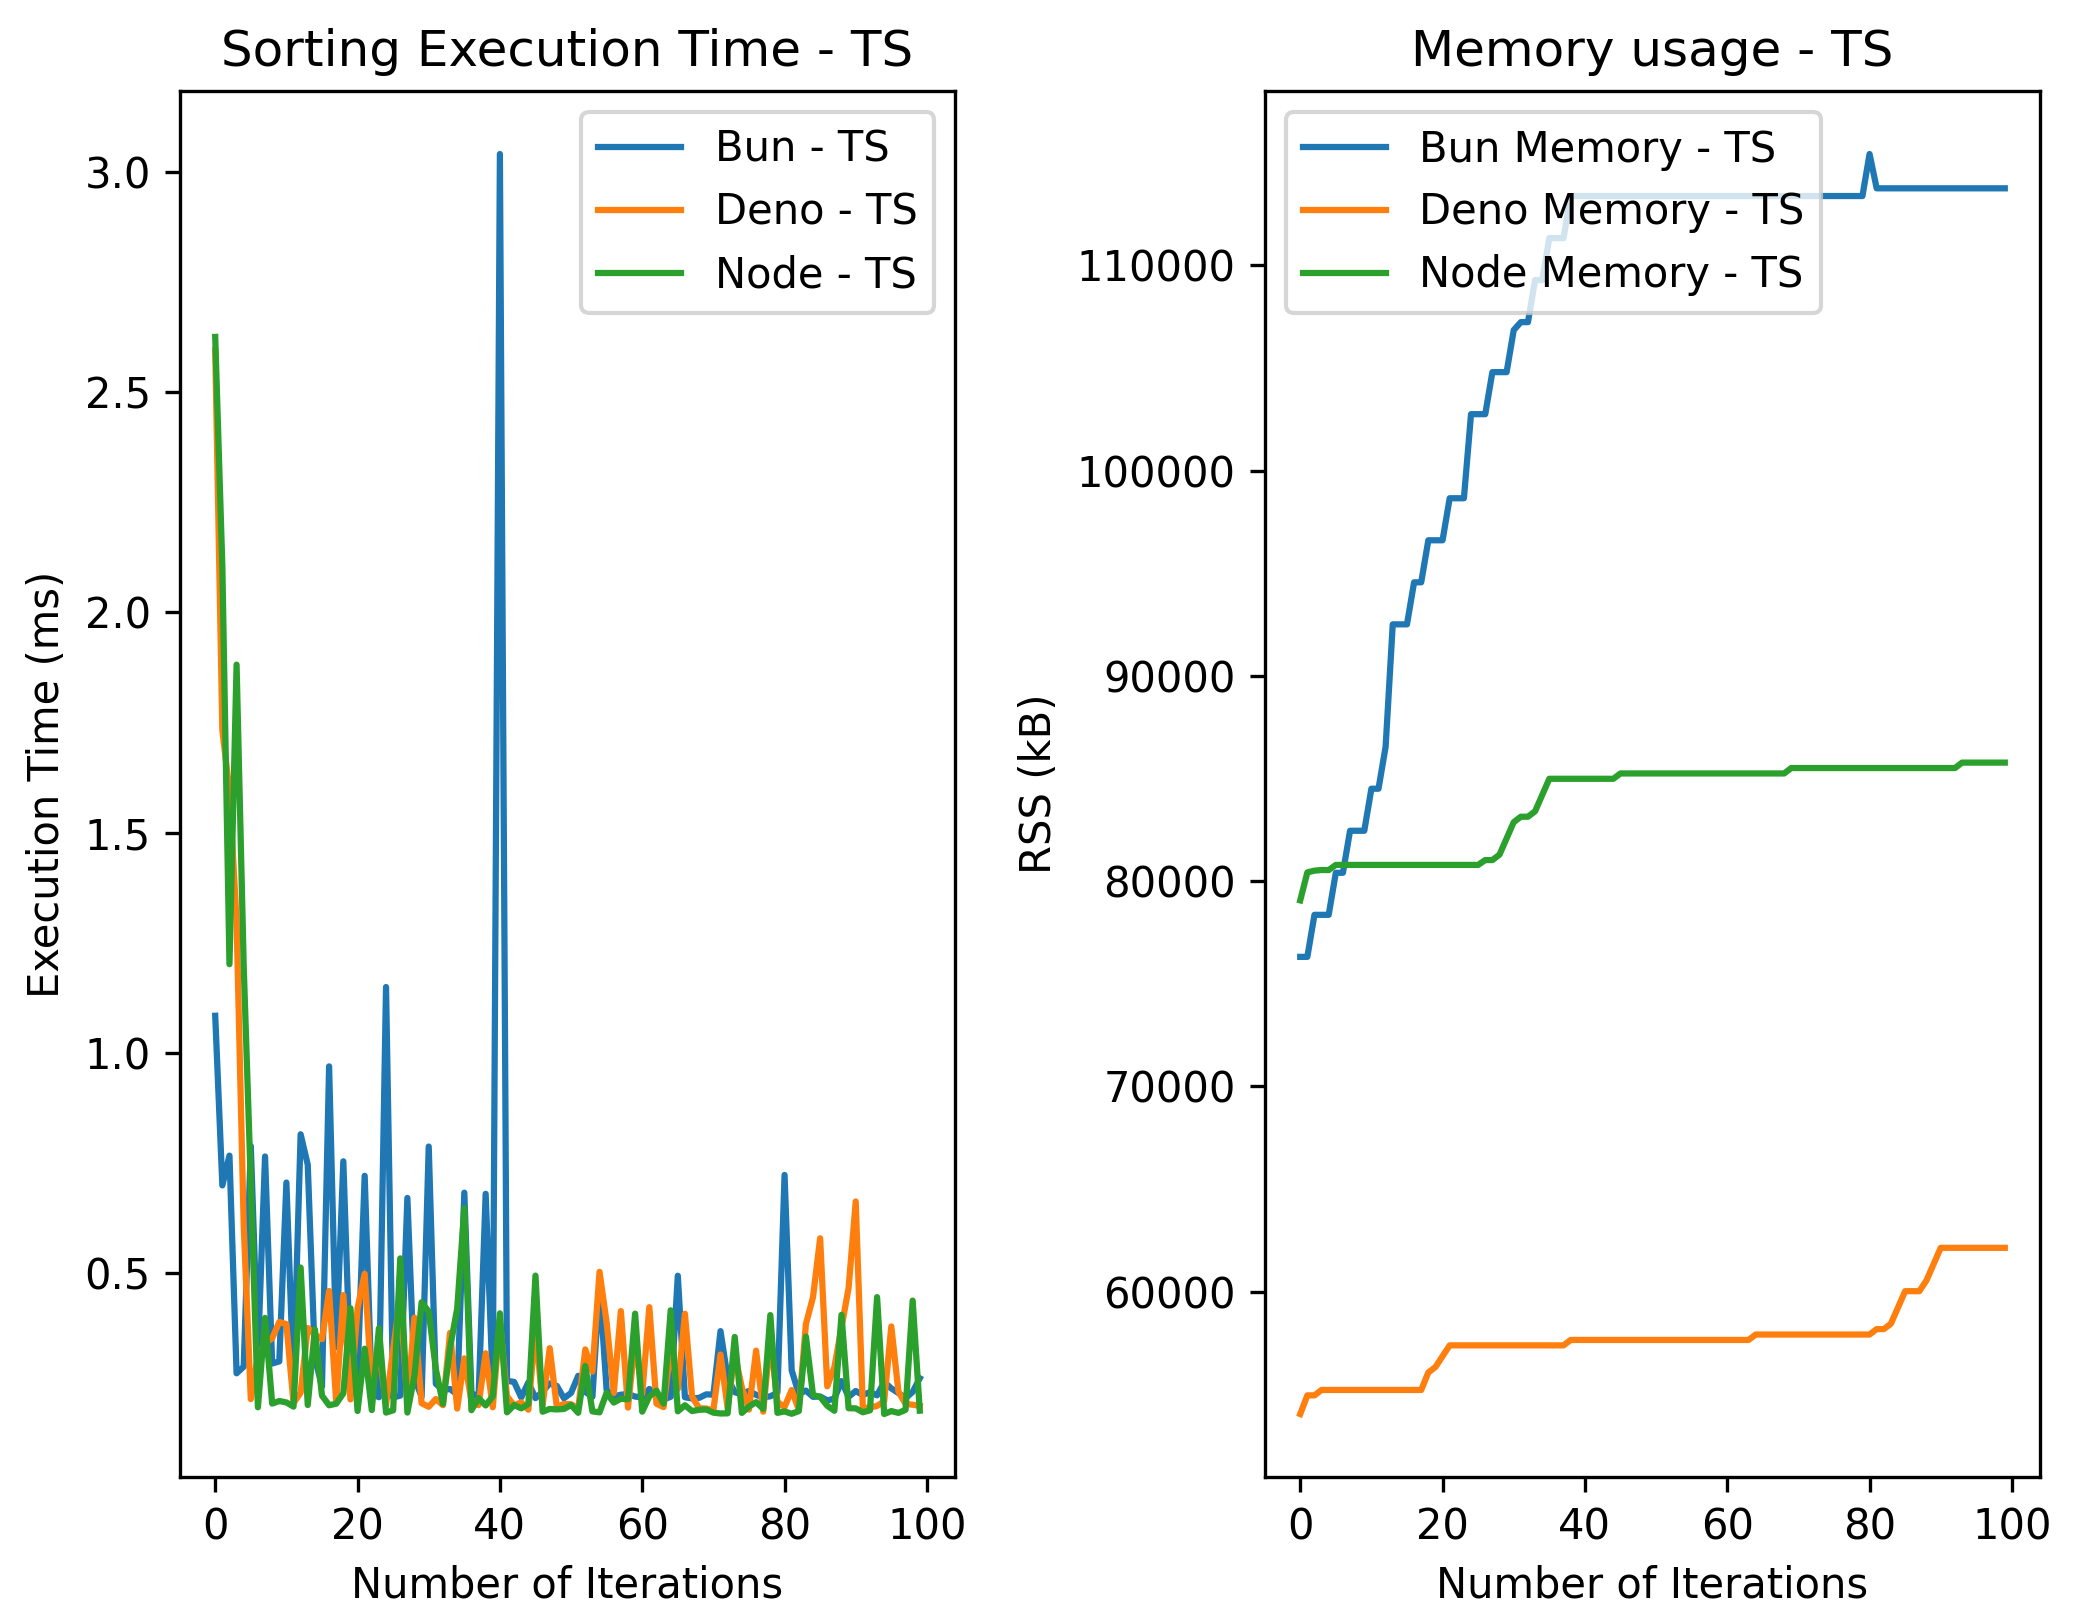
\includegraphics[width=0.7\textwidth]{Figures/sorting/sorting_quick_100_1000_ts.png}
  \caption{Wyniki eksperymentów dla algorytmu sortowania szybkiego dla 100 iteracji i 1000 elementów - po lewej czas wykonania jednorazowego testu w milisekundach, po prawej ilość zajmowanej pamięci w kilobajtach (kB)}
  \label{fig:quick_sorting_e1_ts}
\end{figure}

Na rysunku \ref{fig:quick_sorting_e2} przedstawiono wyniki eksperymentów dla algorytmu sortowania szybkiego dla 100 iteracji i 1000 elementów napisanego w języku JavaScript. Na wykresie przedstawiono czas wykonania jednorazowego testu w milisekundach oraz ilość zajmowanej pamięci w kilobajtach (kB).

\begin{figure}[H]
  \centering
  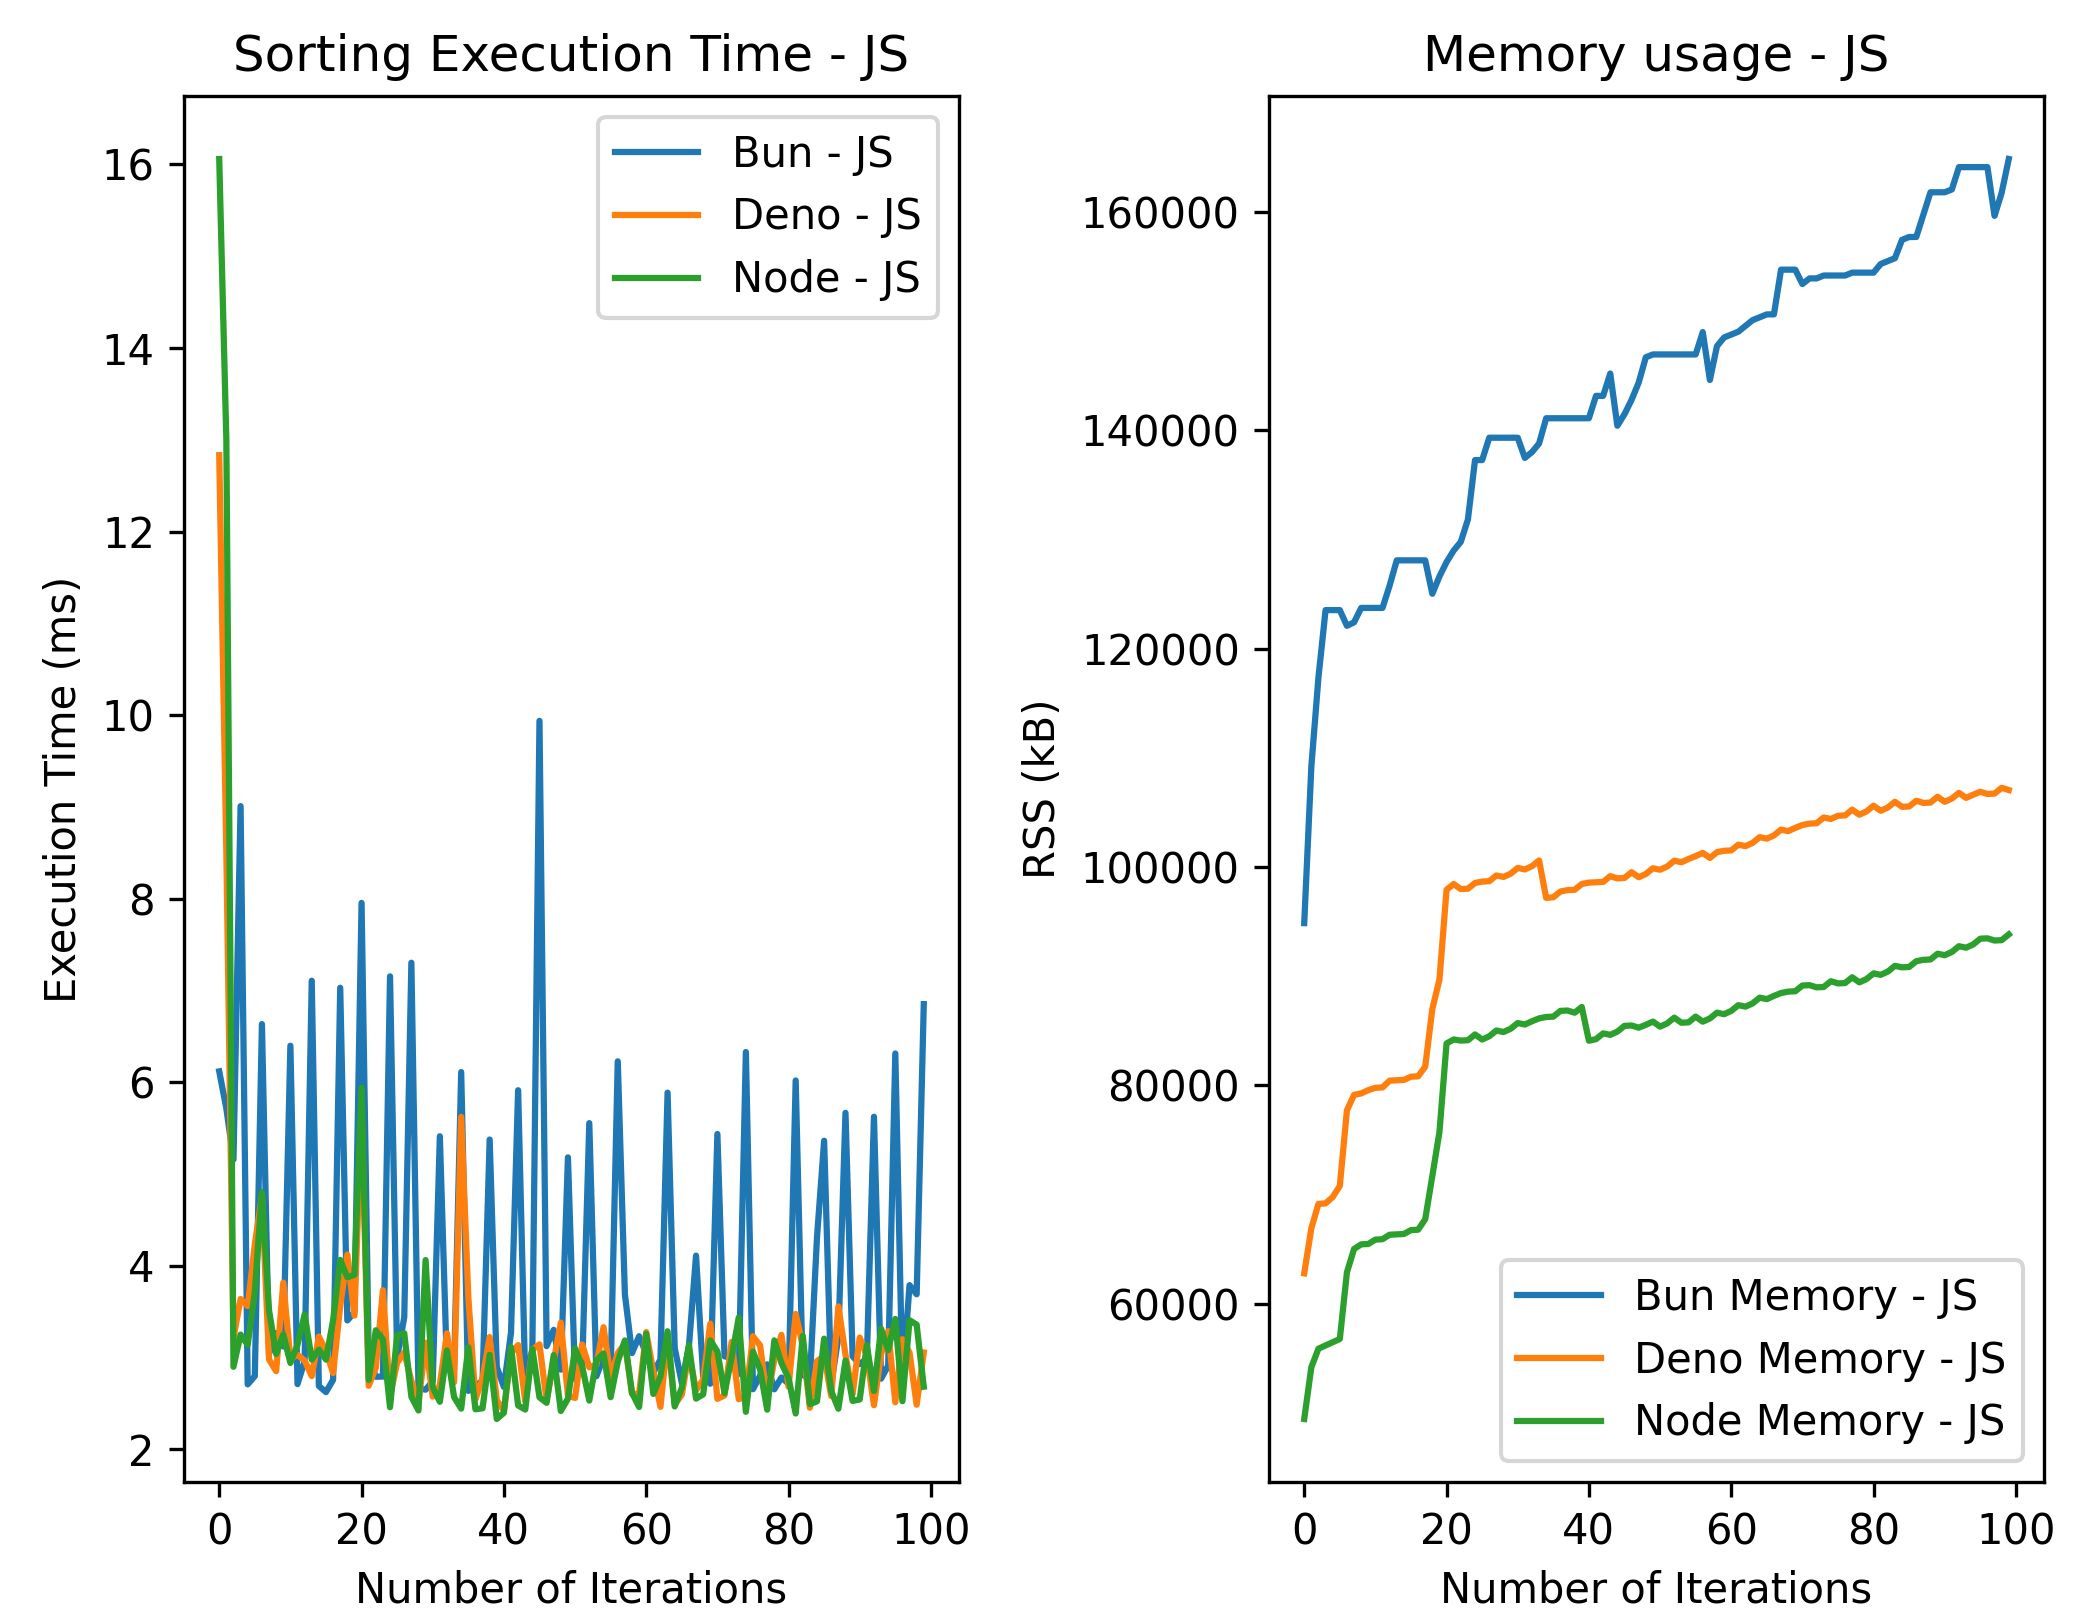
\includegraphics[width=0.7\textwidth]{Figures/sorting/sorting_quick_100_10000_js.png}
  \caption{Wyniki eksperymentów dla algorytmu sortowania szybkiego dla 100 iteracji i 10000 elementów - po lewej czas wykonania jednorazowego testu w milisekundach, po prawej ilość zajmowanej pamięci w kilobajtach (kB)}
  \label{fig:quick_sorting_e2}
\end{figure}

Na rysunku \ref{fig:quick_sorting_e2_ts} przedstawiono wyniki eksperymentów dla algorytmu sortowania szybkiego dla 100 iteracji i 10000 elementów napisanego w języku TypeScript. Na wykresie przedstawiono czas wykonania jednorazowego testu w milisekundach oraz ilość zajmowanej pamięci w kilobajtach (kB).

\begin{figure}[H]
  \centering
  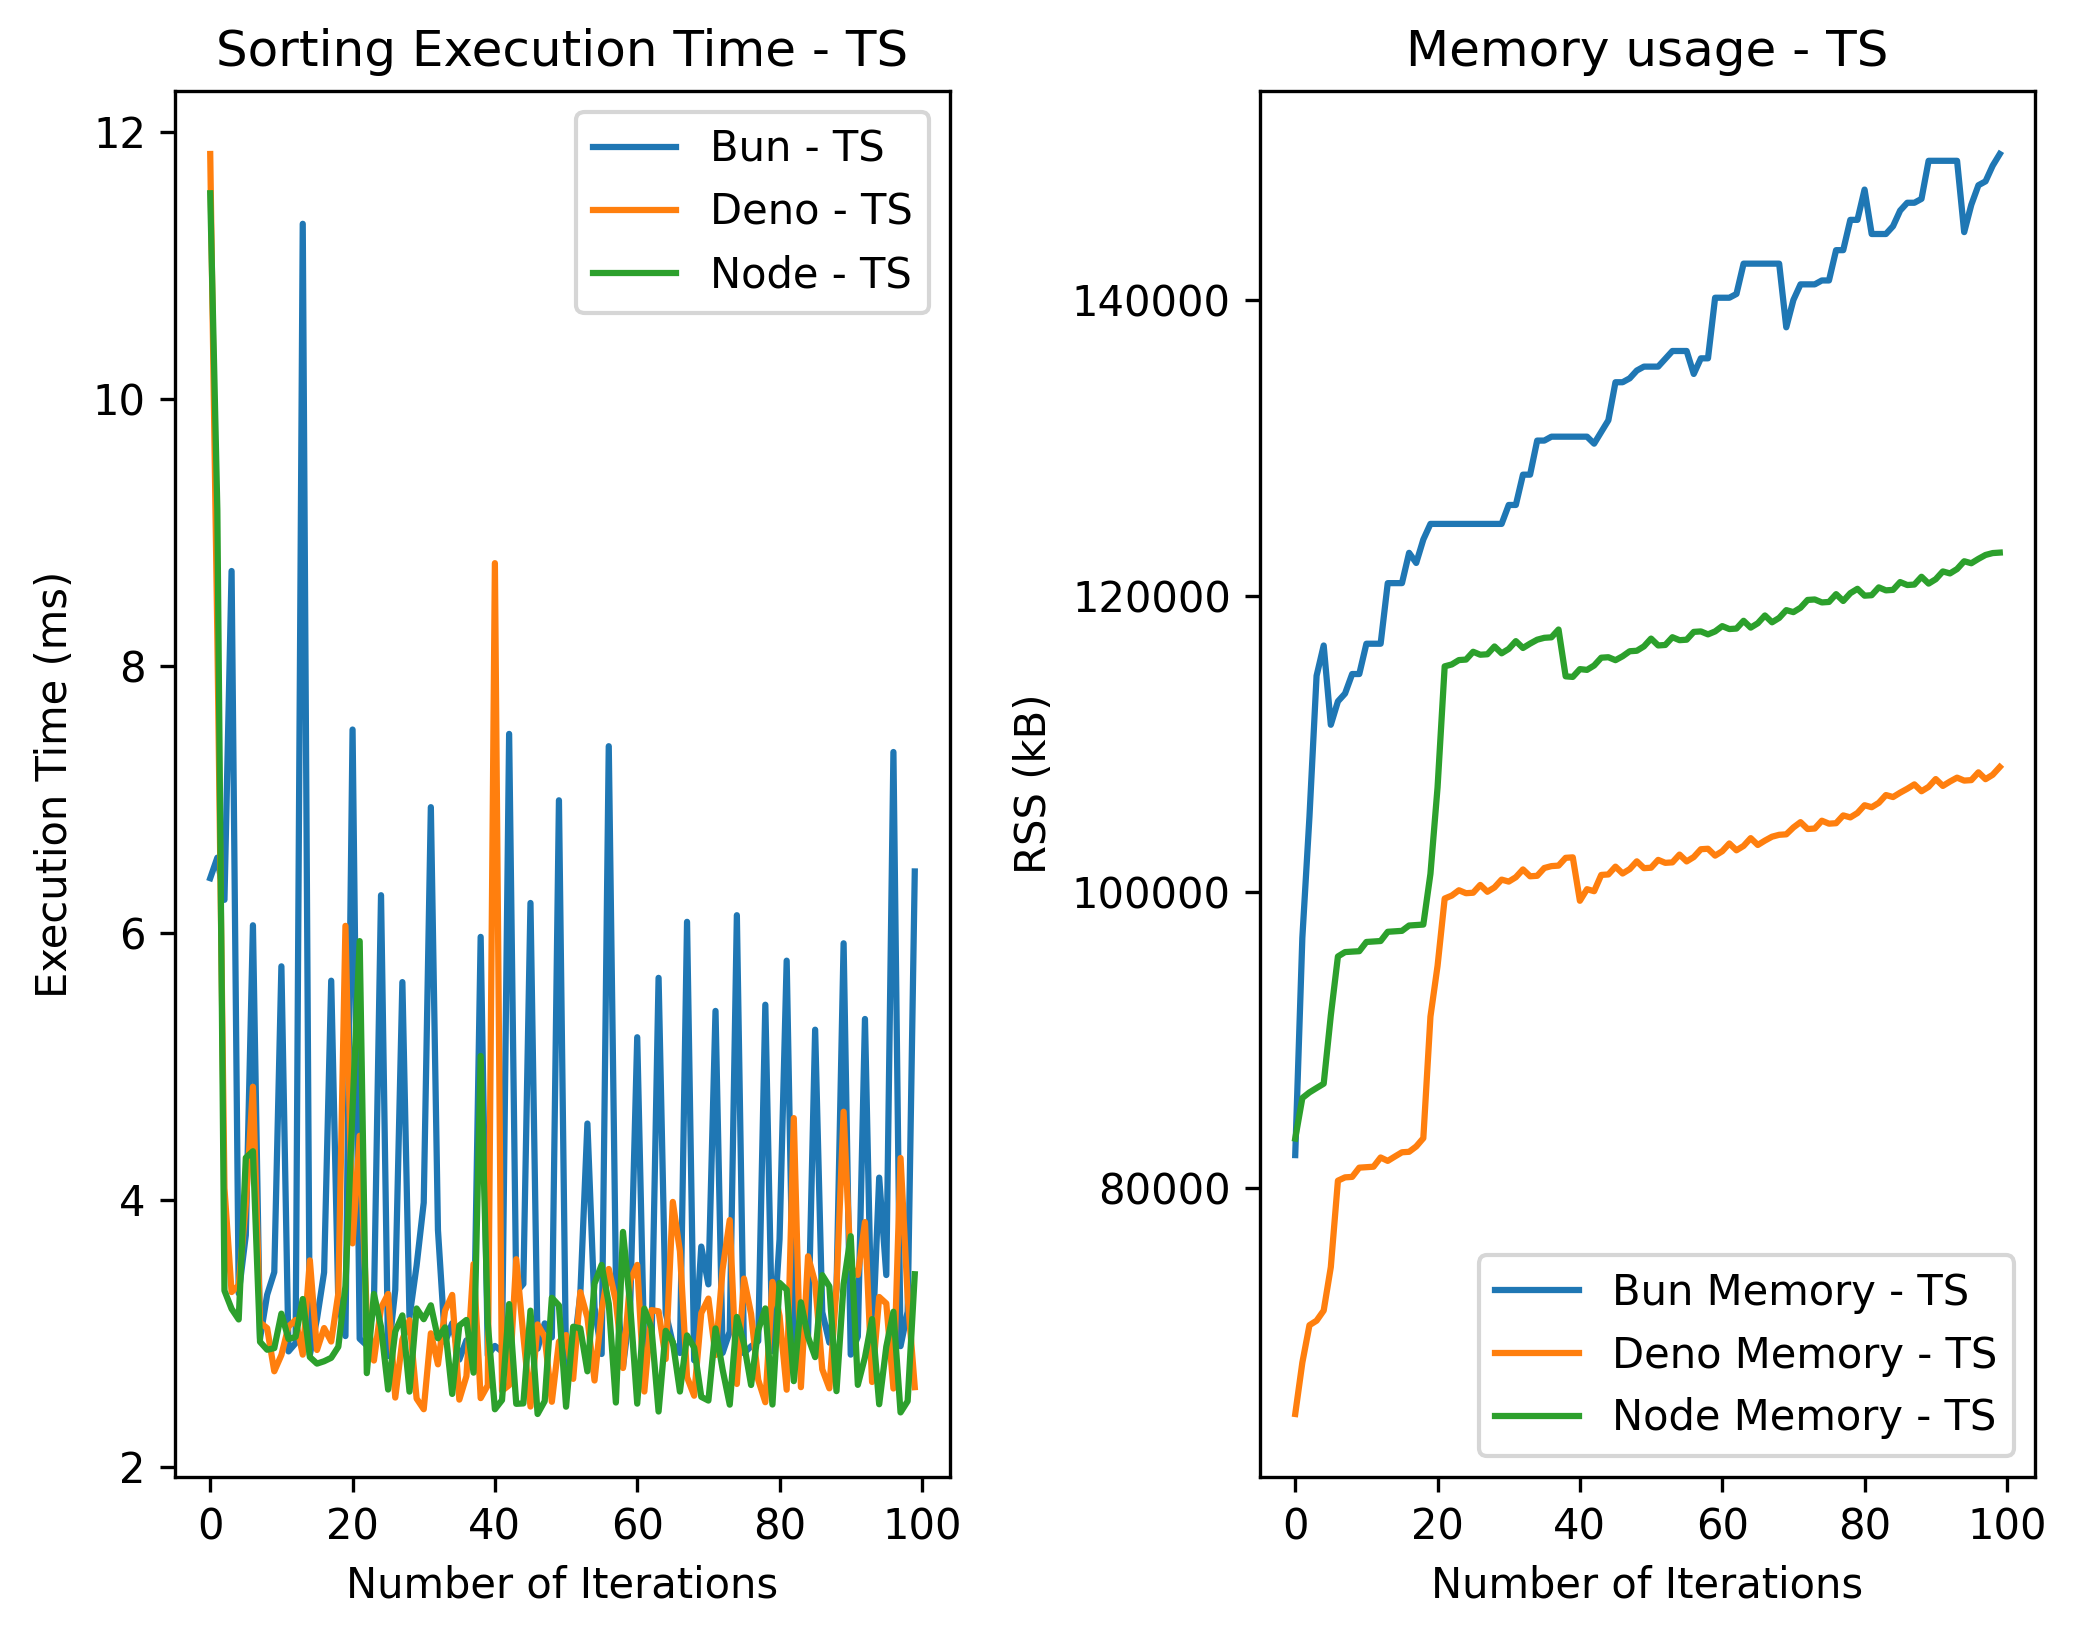
\includegraphics[width=0.7\textwidth]{Figures/sorting/sorting_quick_100_10000_ts.png}
  \caption{Wyniki eksperymentów dla algorytmu sortowania szybkiego dla 100 iteracji i 10000 elementów - po lewej czas wykonania jednorazowego testu w milisekundach, po prawej ilość zajmowanej pamięci w kilobajtach (kB)}
  \label{fig:quick_sorting_e2_ts}
\end{figure}

Na rysunku \ref{fig:quick_sorting_e3} przedstawiono wyniki eksperymentów dla algorytmu sortowania szybkiego dla 1000 iteracji i 1000 elementów napisanego w języku JavaScript. Na wykresie przedstawiono czas wykonania jednorazowego testu w milisekundach oraz ilość zajmowanej pamięci w kilobajtach (kB).

\begin{figure}[H]
  \centering
  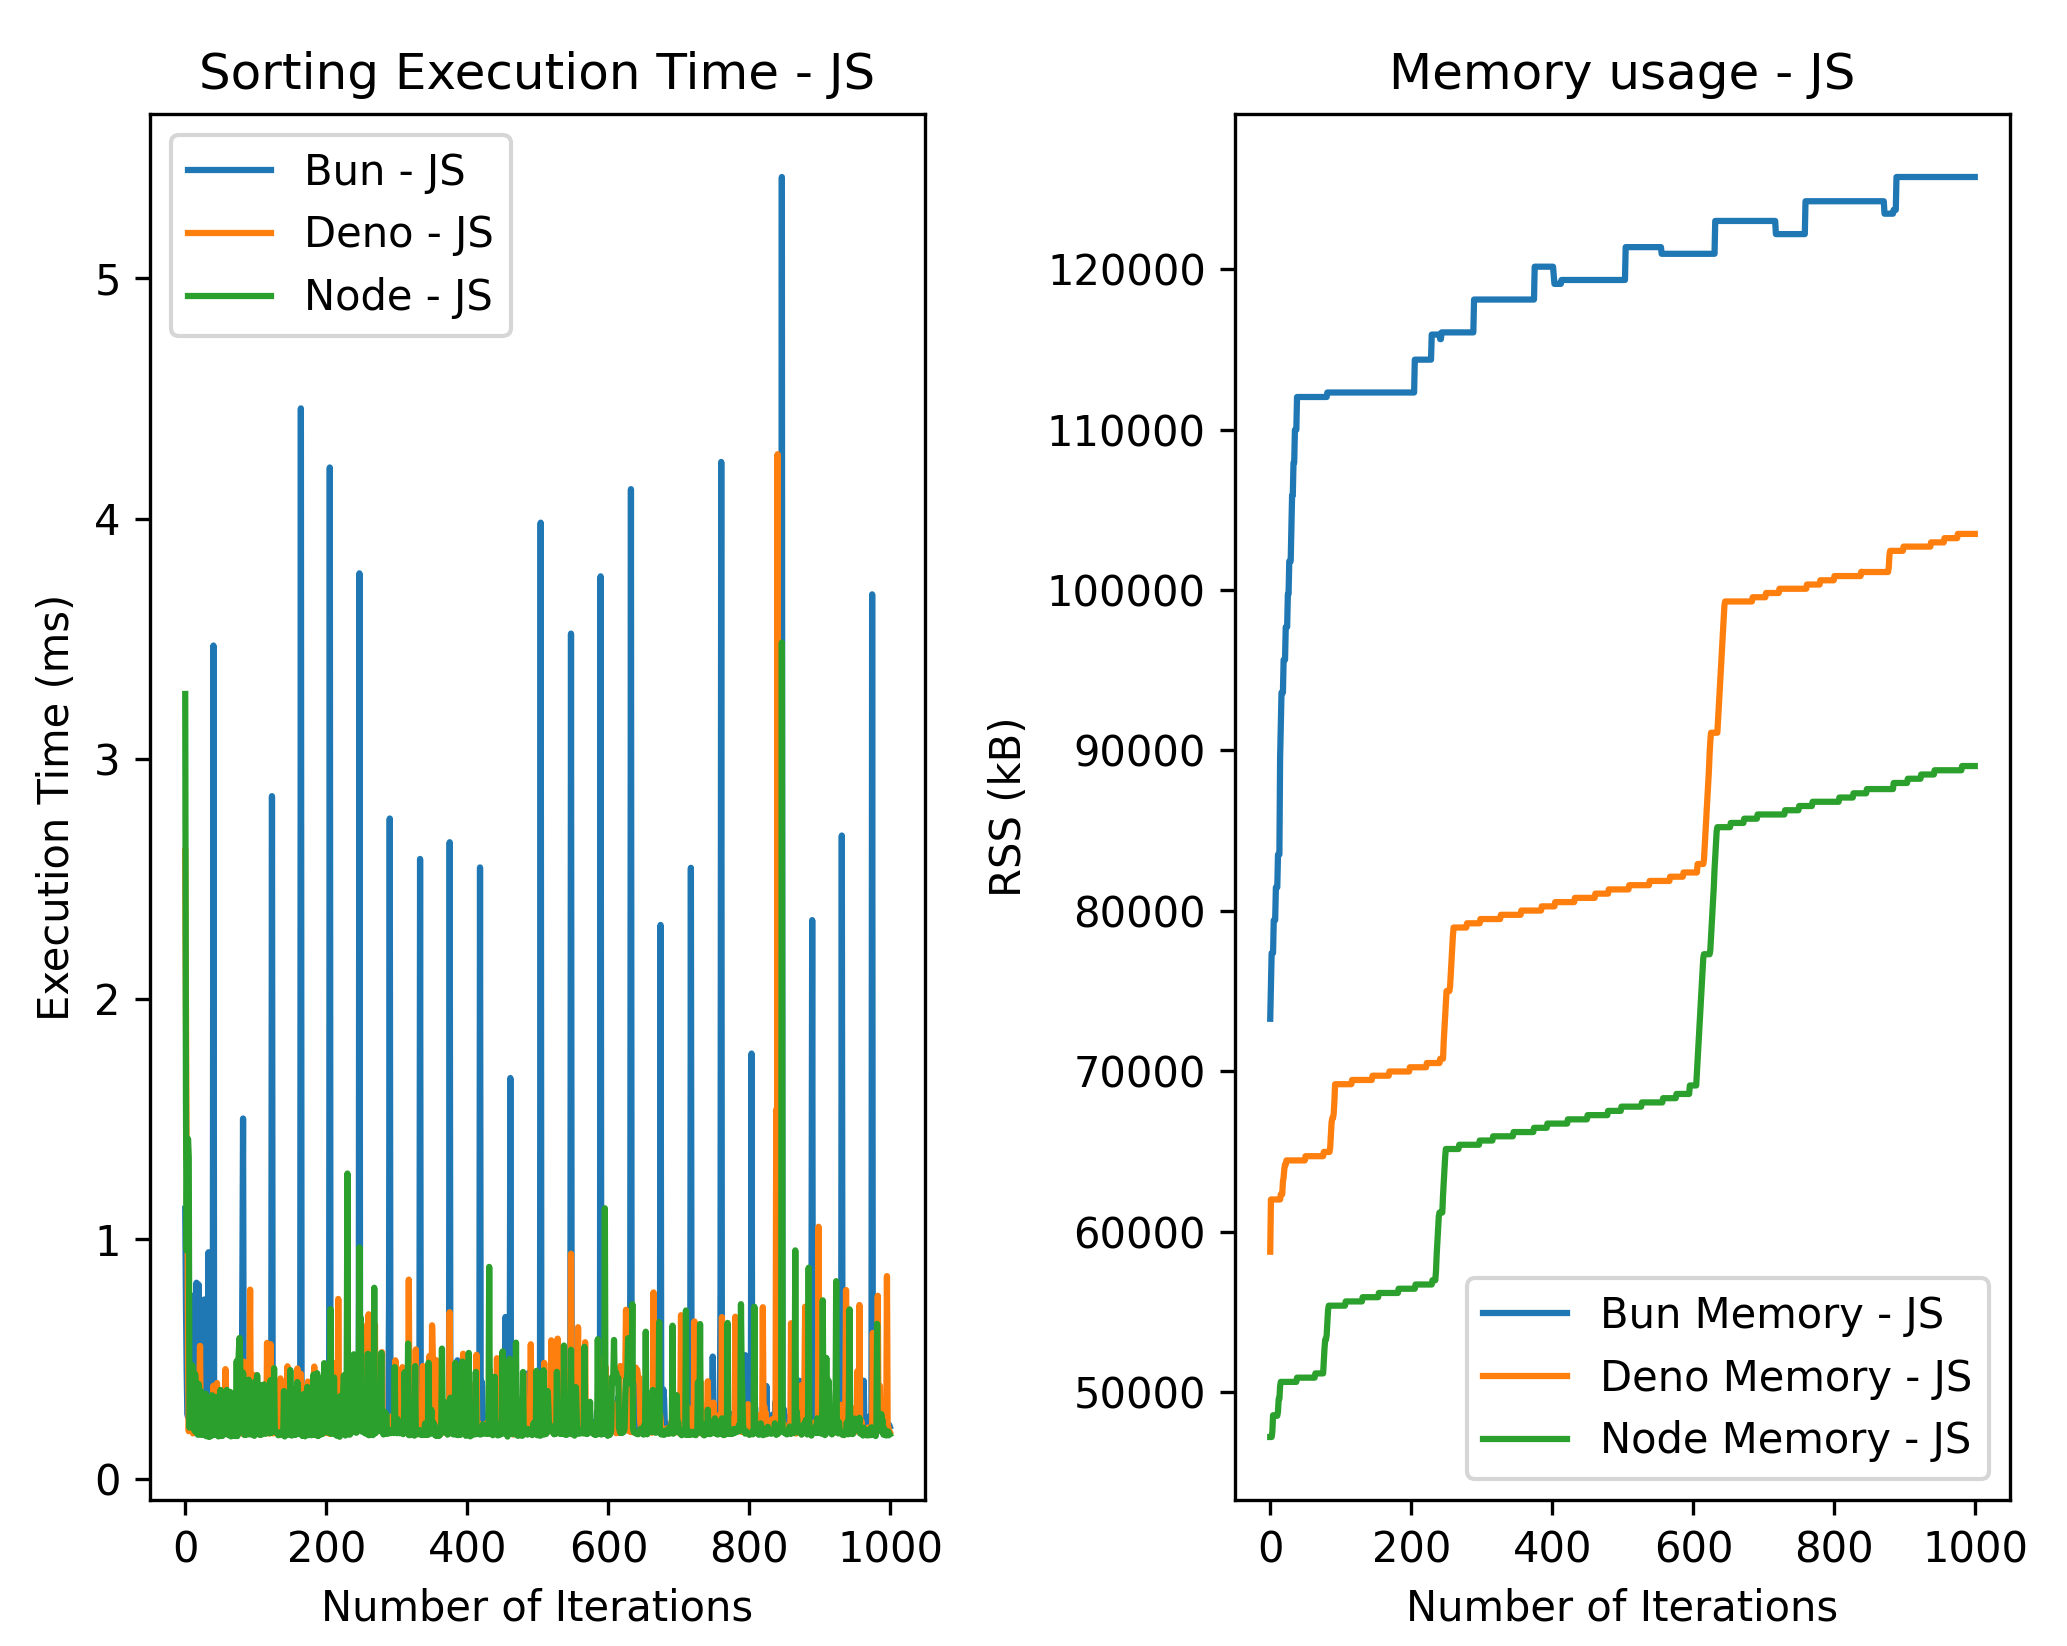
\includegraphics[width=0.7\textwidth]{Figures/sorting/sorting_quick_1000_1000_js.png}
  \caption{Wyniki eksperymentów dla algorytmu sortowania szybkiego dla 1000 iteracji i 1000 elementów - po lewej czas wykonania jednorazowego testu w milisekundach, po prawej ilość zajmowanej pamięci w kilobajtach (kB)}
  \label{fig:quick_sorting_e3}
\end{figure}

Na rysunku \ref{fig:quick_sorting_e3_ts} przedstawiono wyniki eksperymentów dla algorytmu sortowania szybkiego dla 1000 iteracji i 1000 elementów napisanego w języku TypeScript. Na wykresie przedstawiono czas wykonania jednorazowego testu w milisekundach oraz ilość zajmowanej pamięci w kilobajtach (kB).

\begin{figure}[H]
  \centering
  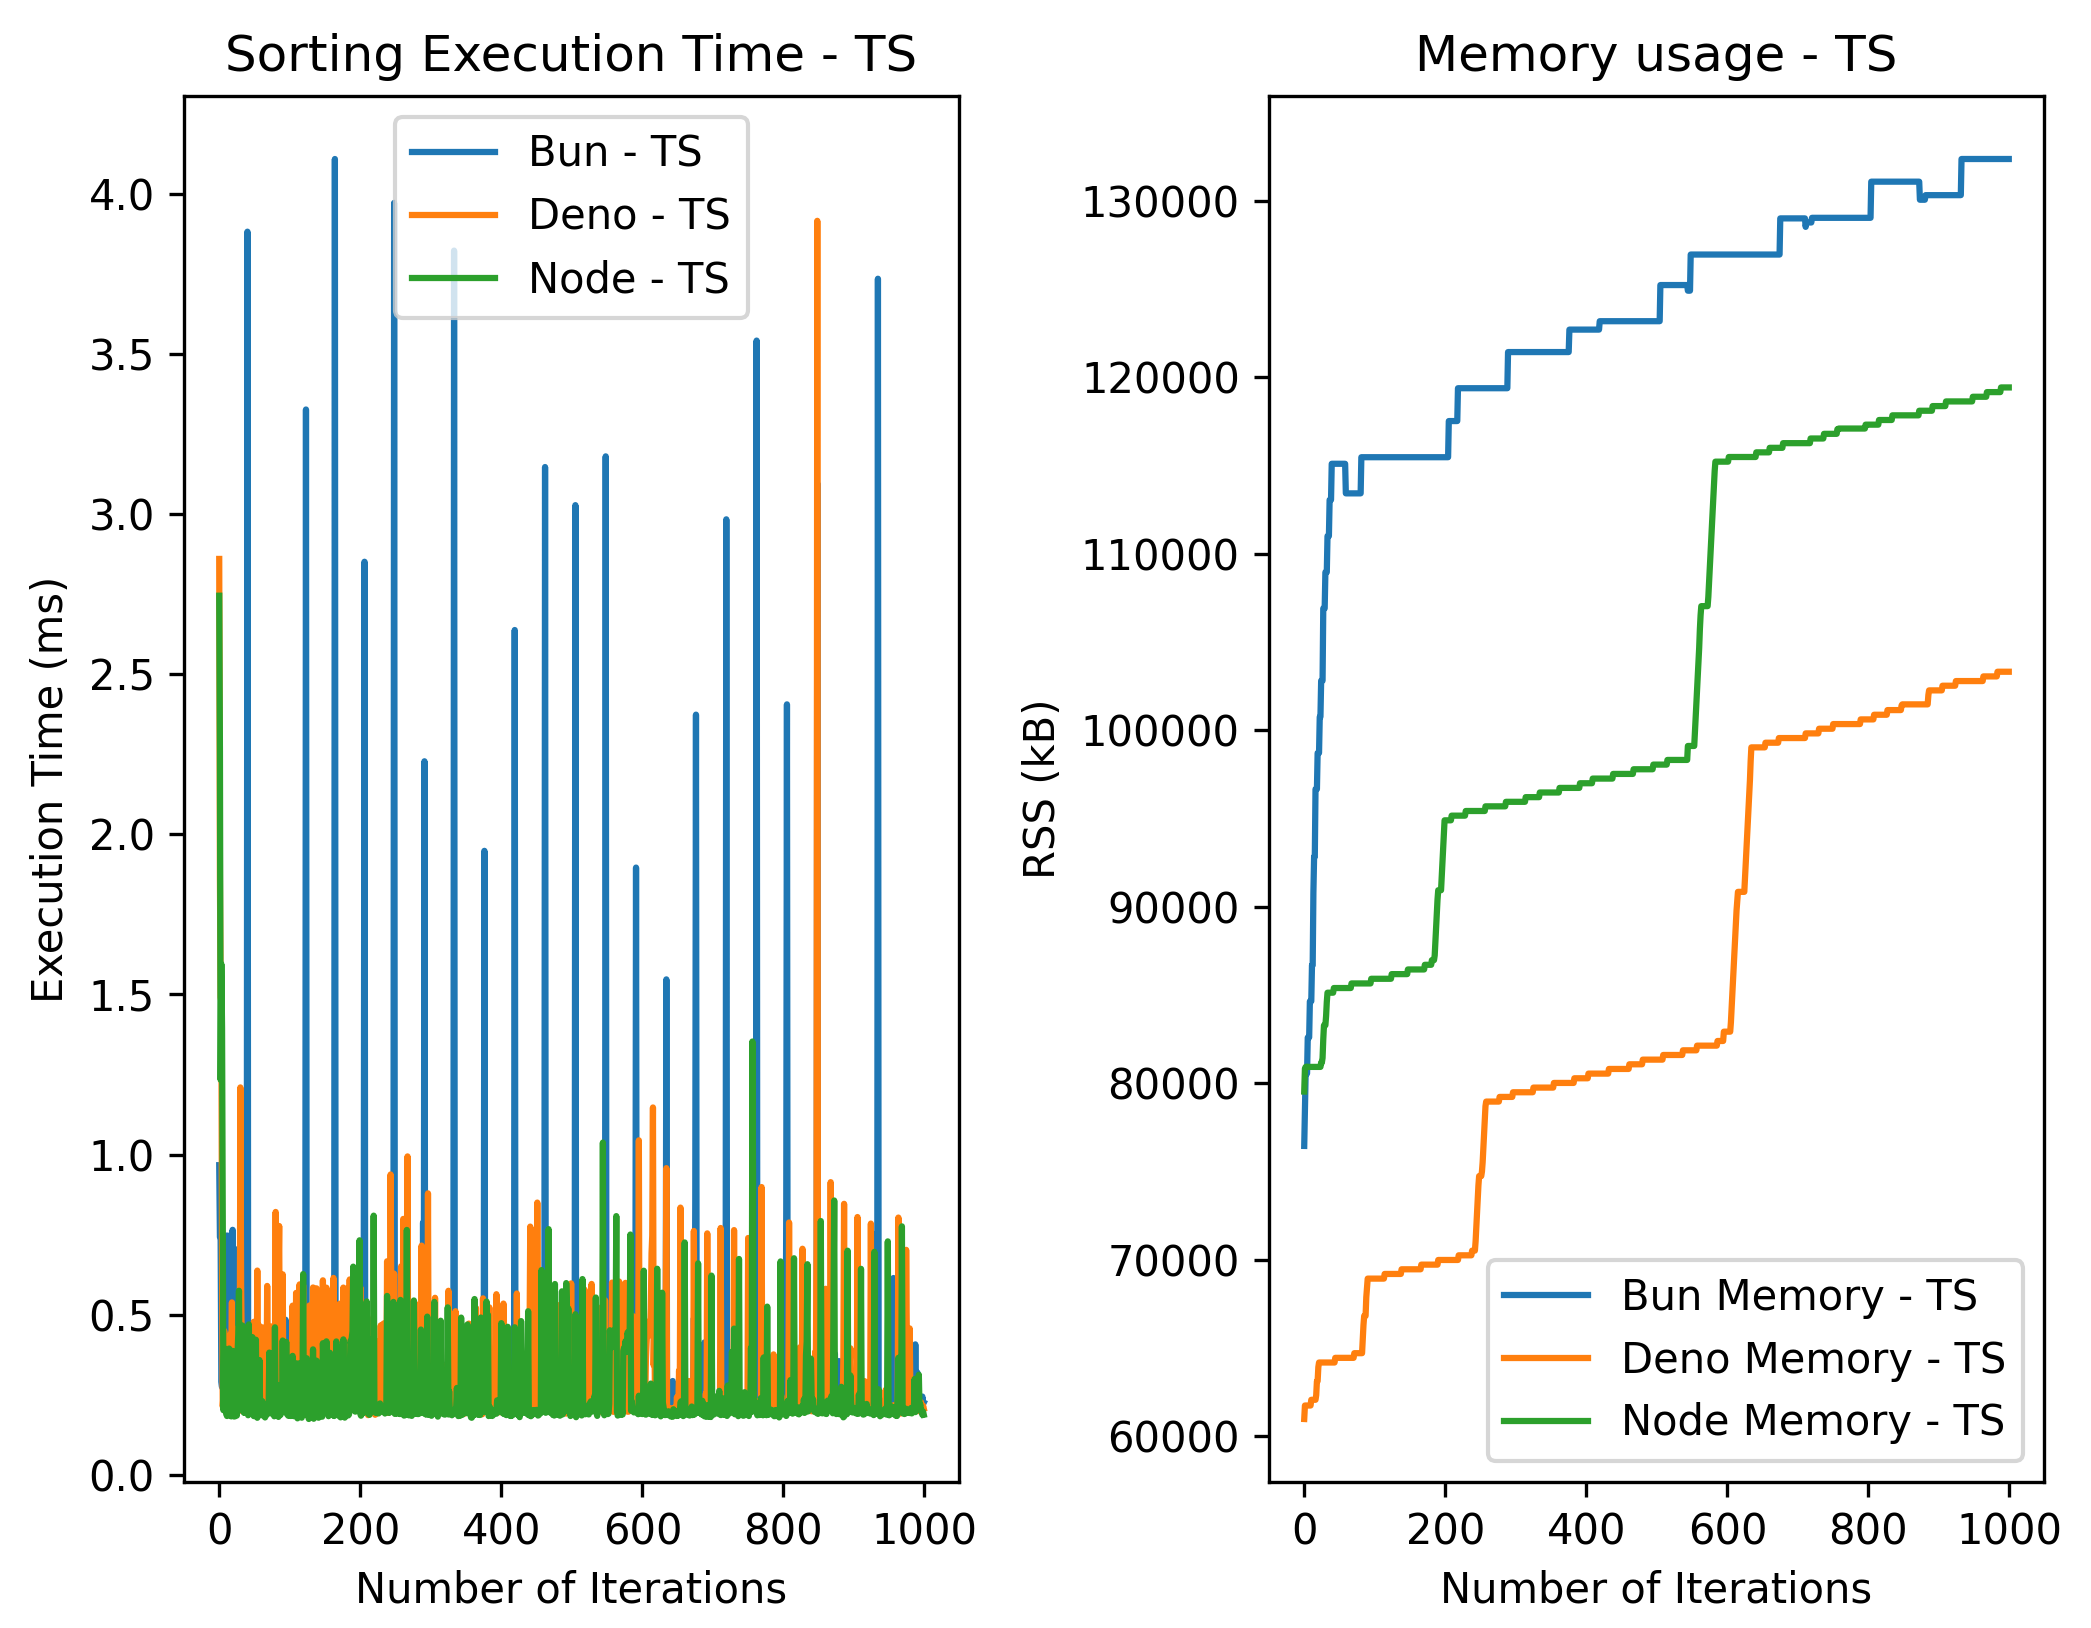
\includegraphics[width=0.7\textwidth]{Figures/sorting/sorting_quick_1000_1000_ts.png}
  \caption{Wyniki eksperymentów dla algorytmu sortowania szybkiego dla 100 iteracji i 1000 elementów - po lewej czas wykonania jednorazowego testu w milisekundach, po prawej ilość zajmowanej pamięci w kilobajtach (kB)}
  \label{fig:quick_sorting_e3_ts}
\end{figure}

Na rysunku \ref{fig:quick_sorting_e4} przedstawiono wyniki eksperymentów dla algorytmu sortowania szybkiego dla 100 iteracji i 1000 elementów napisanego w języku JavaScript. Na wykresie przedstawiono czas wykonania jednorazowego testu w milisekundach oraz ilość zajmowanej pamięci w kilobajtach (kB).

\begin{figure}[H]
  \centering
  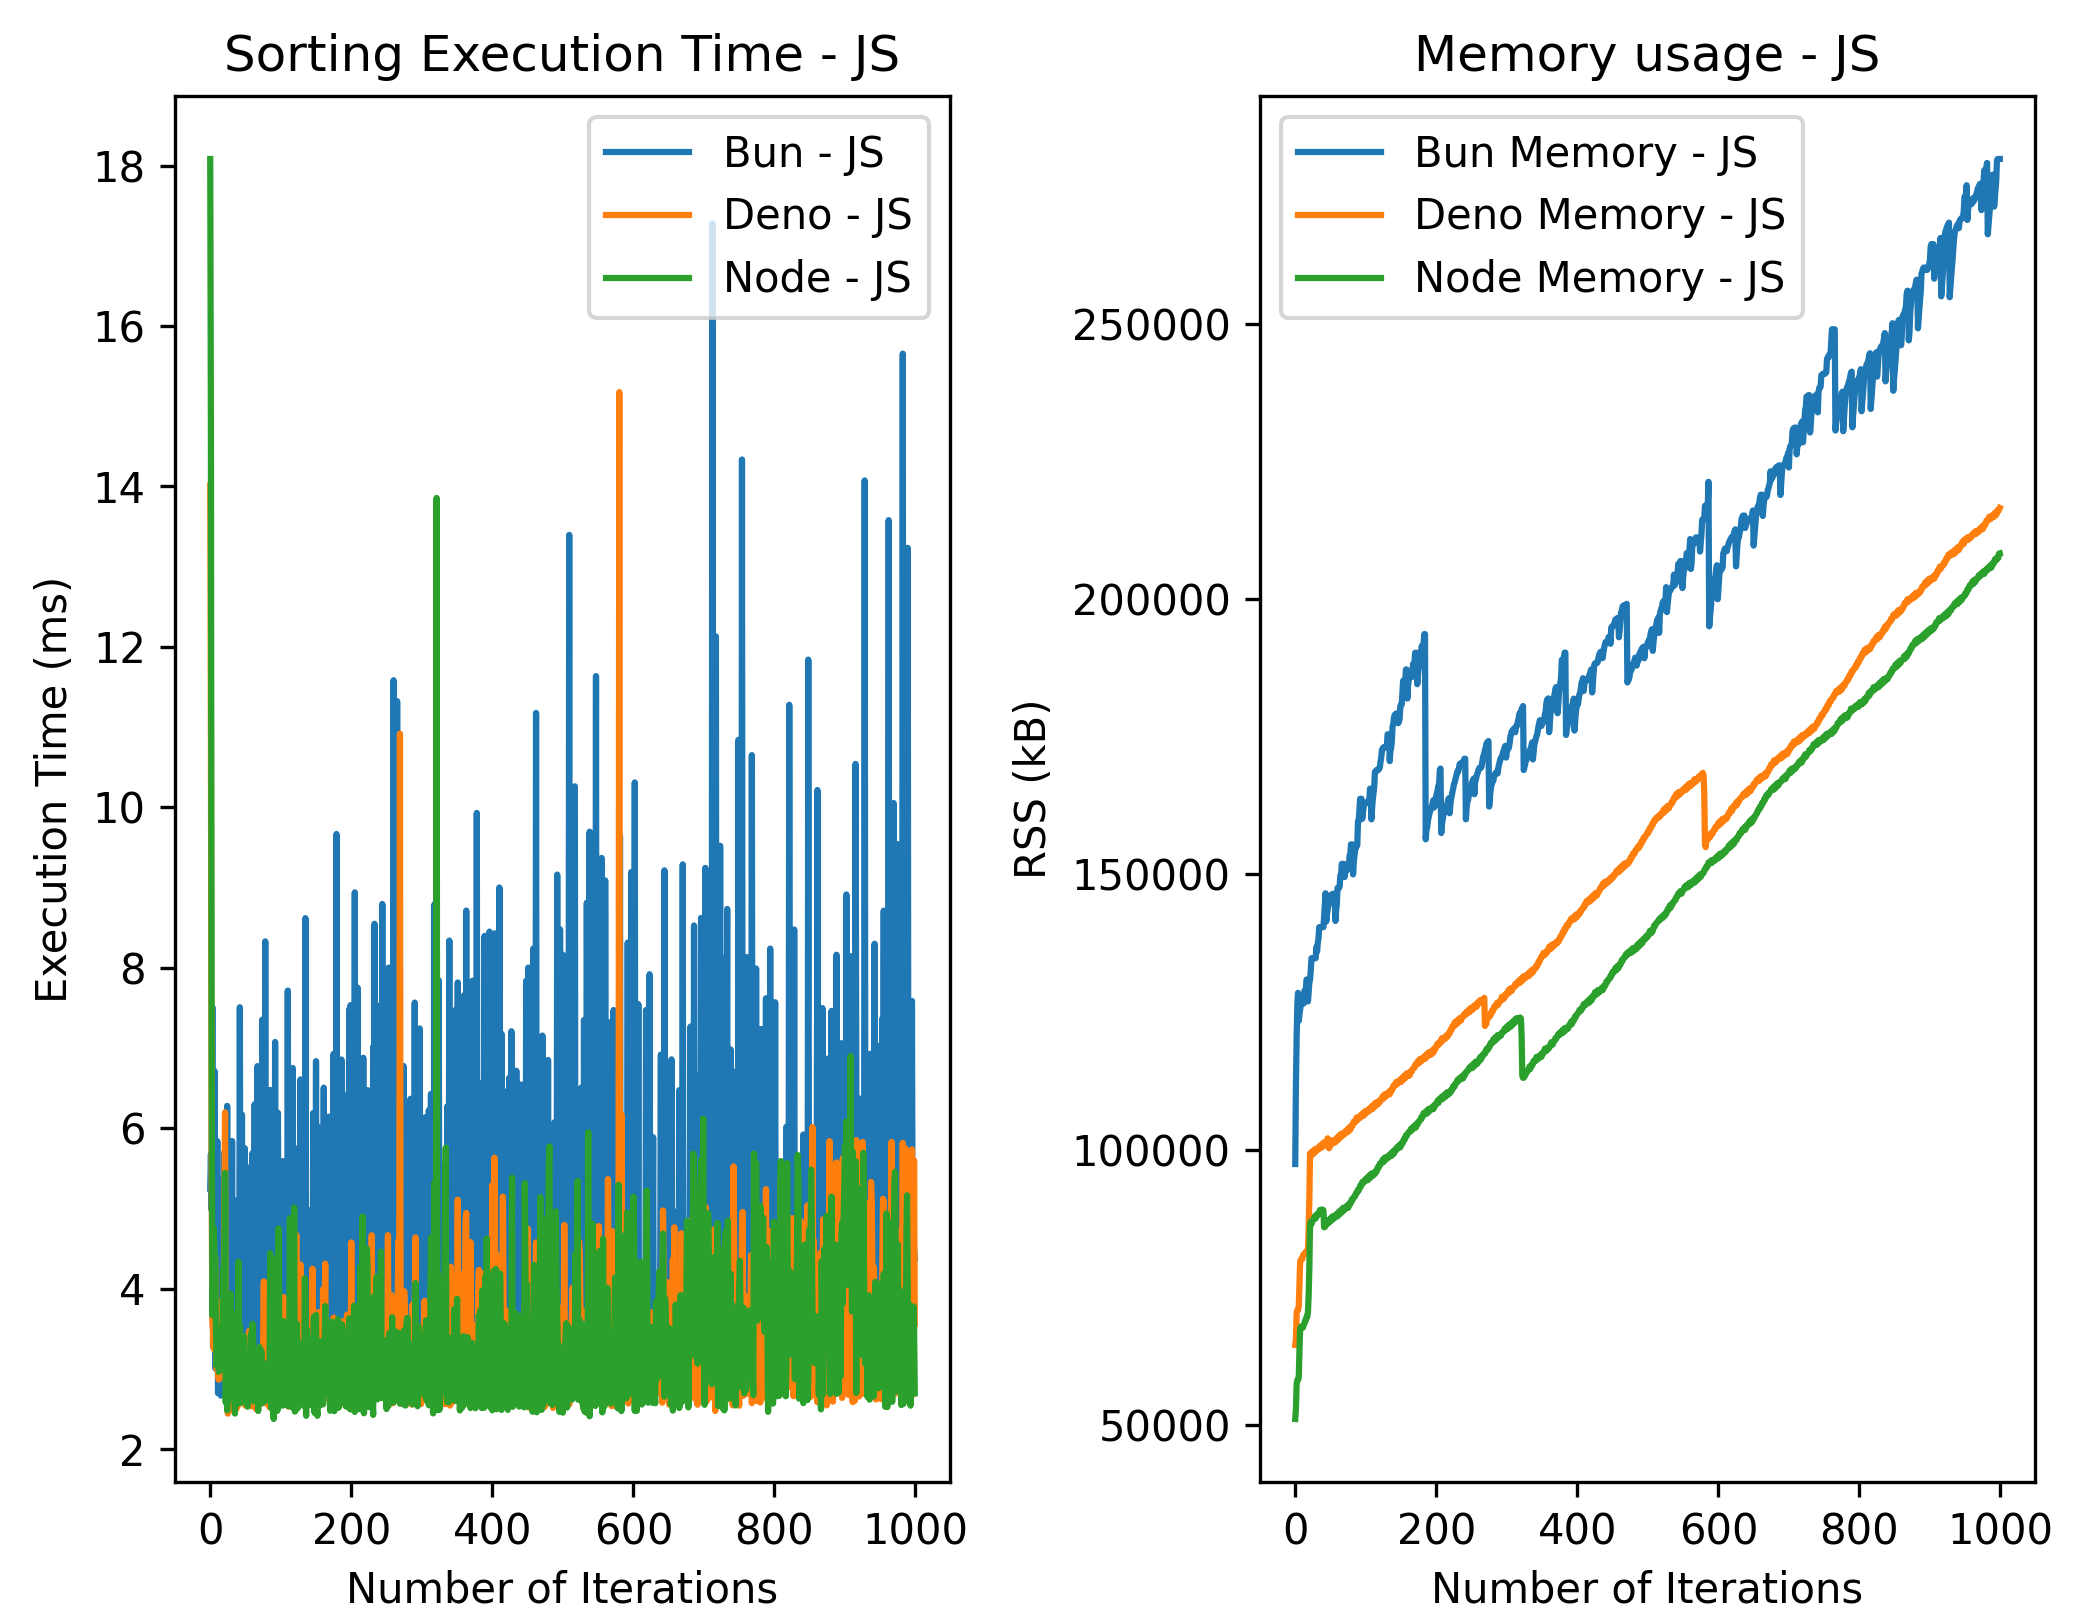
\includegraphics[width=0.7\textwidth]{Figures/sorting/sorting_quick_1000_10000_js.png}
  \caption{Wyniki eksperymentów dla algorytmu sortowania szybkiego dla 100 iteracji i 10000 elementów - po lewej czas wykonania jednorazowego testu w milisekundach, po prawej ilość zajmowanej pamięci w kilobajtach (kB)}
  \label{fig:quick_sorting_e4}
\end{figure}

Na rysunku \ref{fig:quick_sorting_e4_ts} przedstawiono wyniki eksperymentów dla algorytmu sortowania szybkiego dla 100 iteracji i 10000 elementów napisanego w języku TypeScript. Na wykresie przedstawiono czas wykonania jednorazowego testu w milisekundach oraz ilość zajmowanej pamięci w kilobajtach (kB).

\begin{figure}[H]
  \centering
  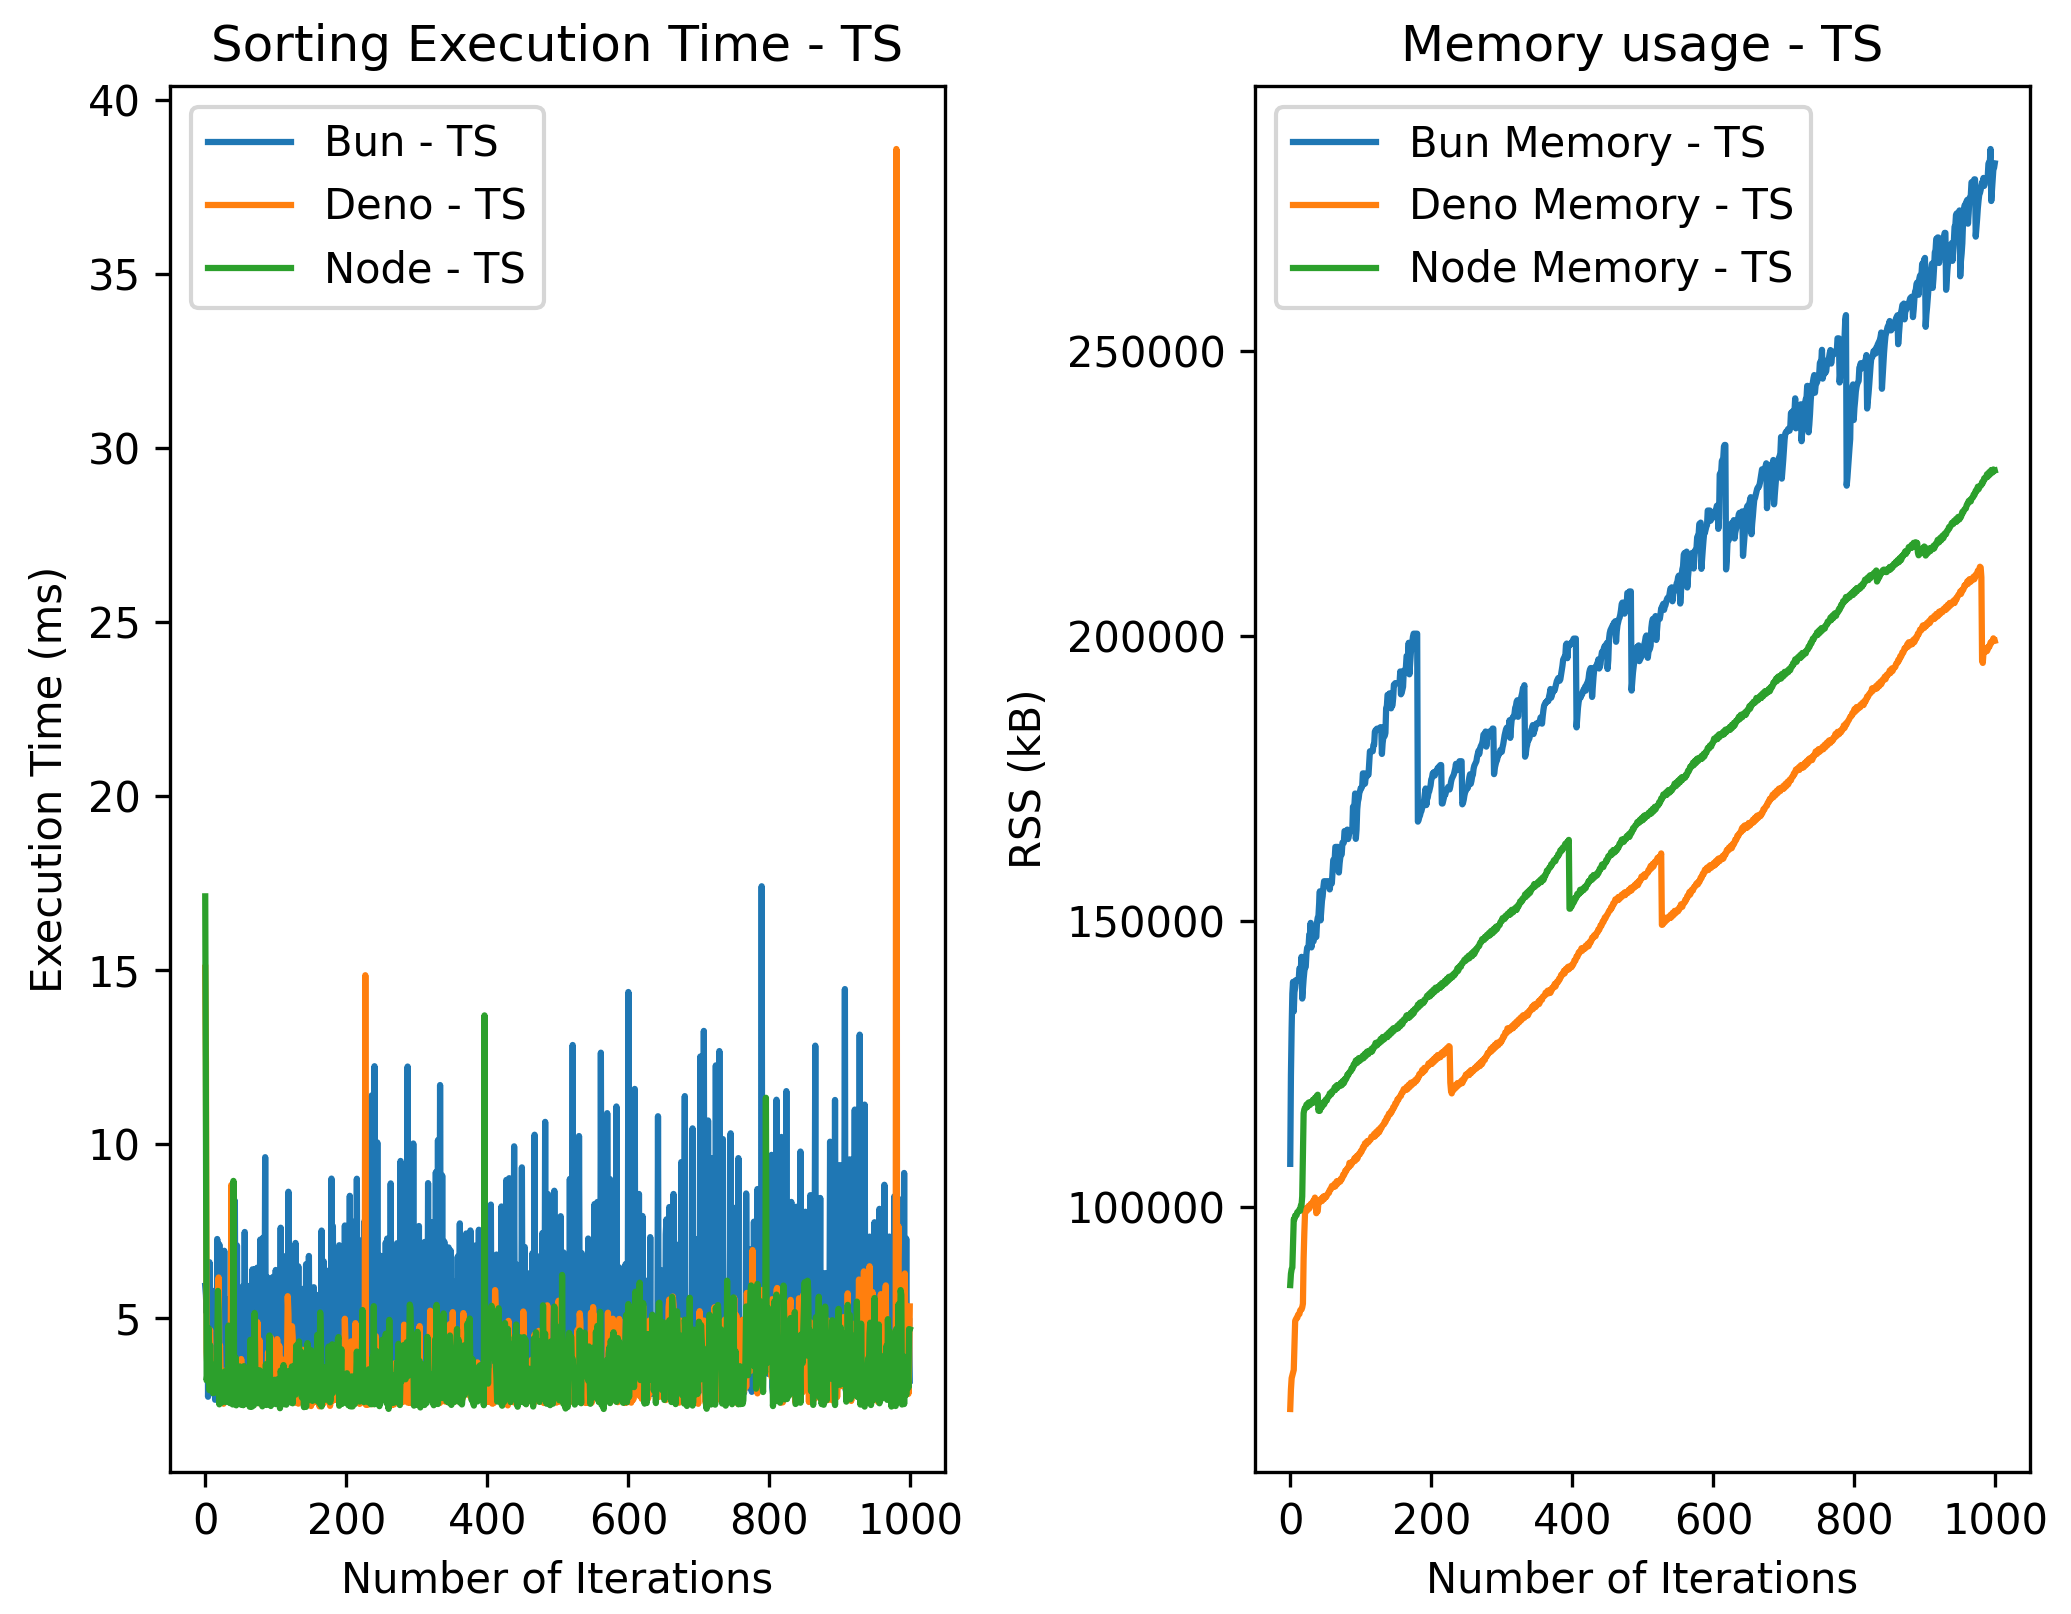
\includegraphics[width=0.7\textwidth]{Figures/sorting/sorting_quick_1000_10000_ts.png}
  \caption{Wyniki eksperymentów dla algorytmu sortowania szybkiego dla 100 iteracji i 10000 elementów - po lewej czas wykonania jednorazowego testu w milisekundach, po prawej ilość zajmowanej pamięci w kilobajtach (kB)}
  \label{fig:quick_sorting_e4_ts}
\end{figure}

\subsubsection{Wyniki - sortowanie pozycyjne}
Na rysunku \ref{fig:radix_sorting_e1} przedstawiono wyniki eksperymentów dla algorytmu sortowania  dla 100 iteracji i 1000 elementów napisanego w języku JavaScript. Na wykresie przedstawiono czas wykonania jednorazowego testu w milisekundach oraz ilość zajmowanej pamięci w kilobajtach (kB).

\begin{figure}[H]
  \centering
  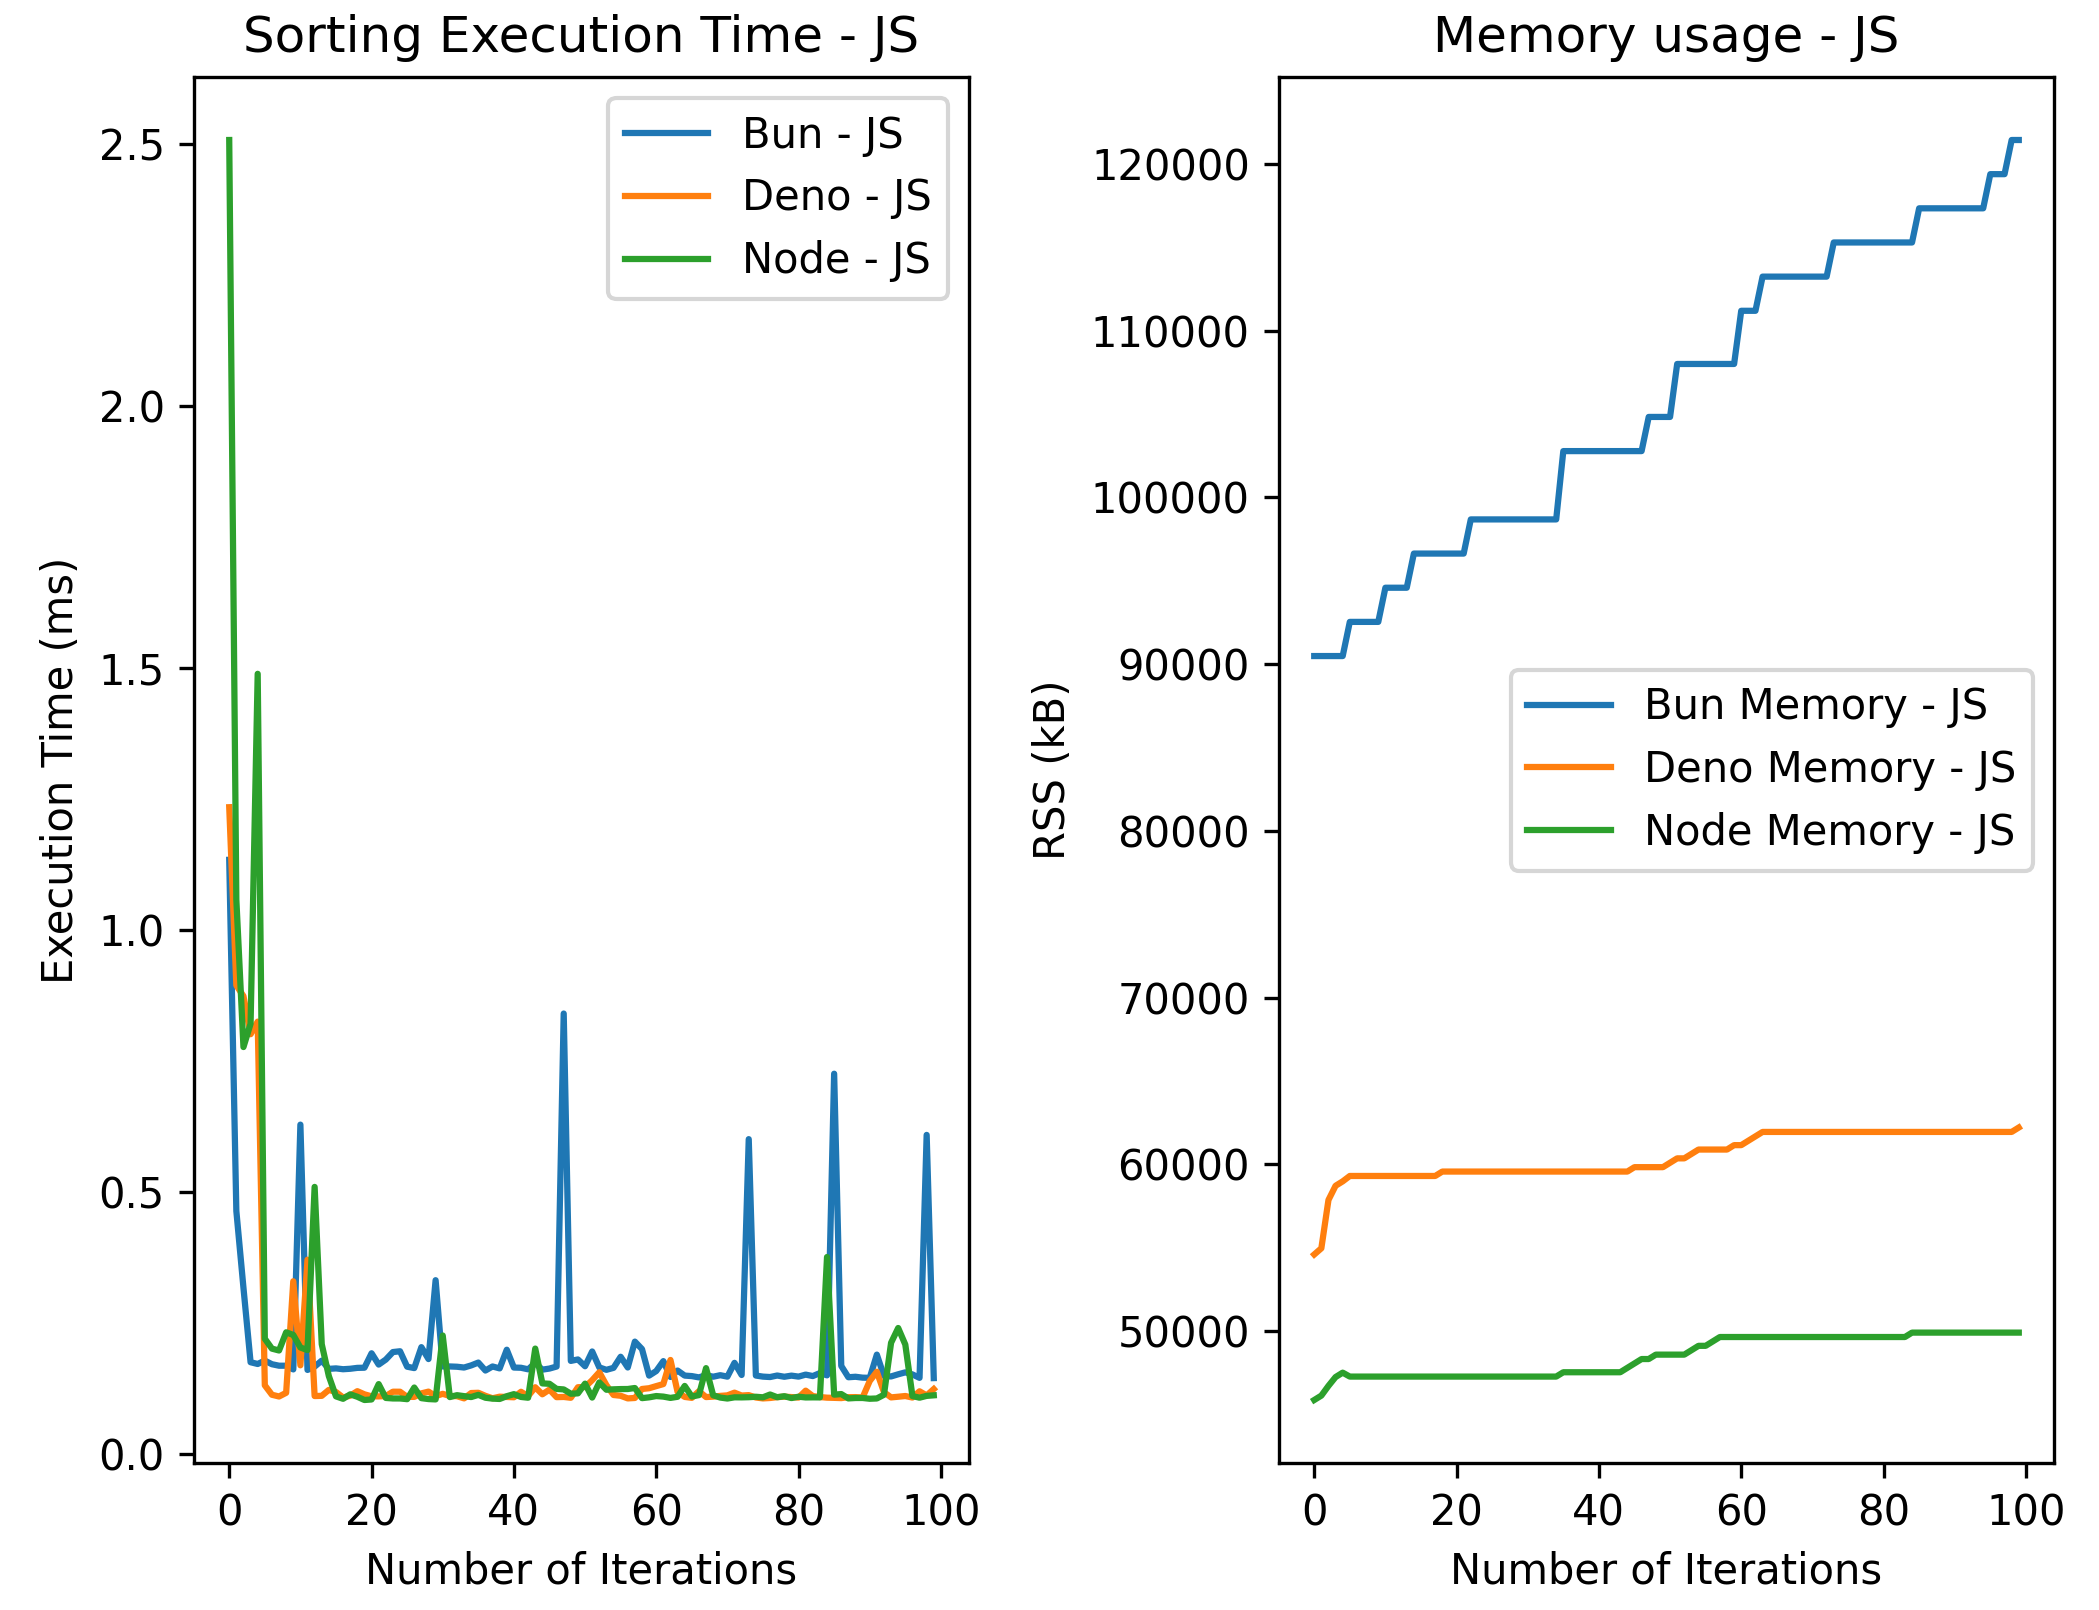
\includegraphics[width=0.7\textwidth]{Figures/sorting/sorting_radix_100_1000_js.png}
  \caption{Wyniki eksperymentów dla algorytmu sortowania  dla 100 iteracji i 1000 elementów - po lewej czas wykonania jednorazowego testu w milisekundach, po prawej ilość zajmowanej pamięci w kilobajtach (kB)}
  \label{fig:radix_sorting_e1}
\end{figure}

Na rysunku \ref{fig:radix_sorting_e1_ts} przedstawiono wyniki eksperymentów dla algorytmu sortowania  dla 100 iteracji i 1000 elementów napisanego w języku TypeScript. Na wykresie przedstawiono czas wykonania jednorazowego testu w milisekundach oraz ilość zajmowanej pamięci w kilobajtach (kB).

\begin{figure}[H]
  \centering
  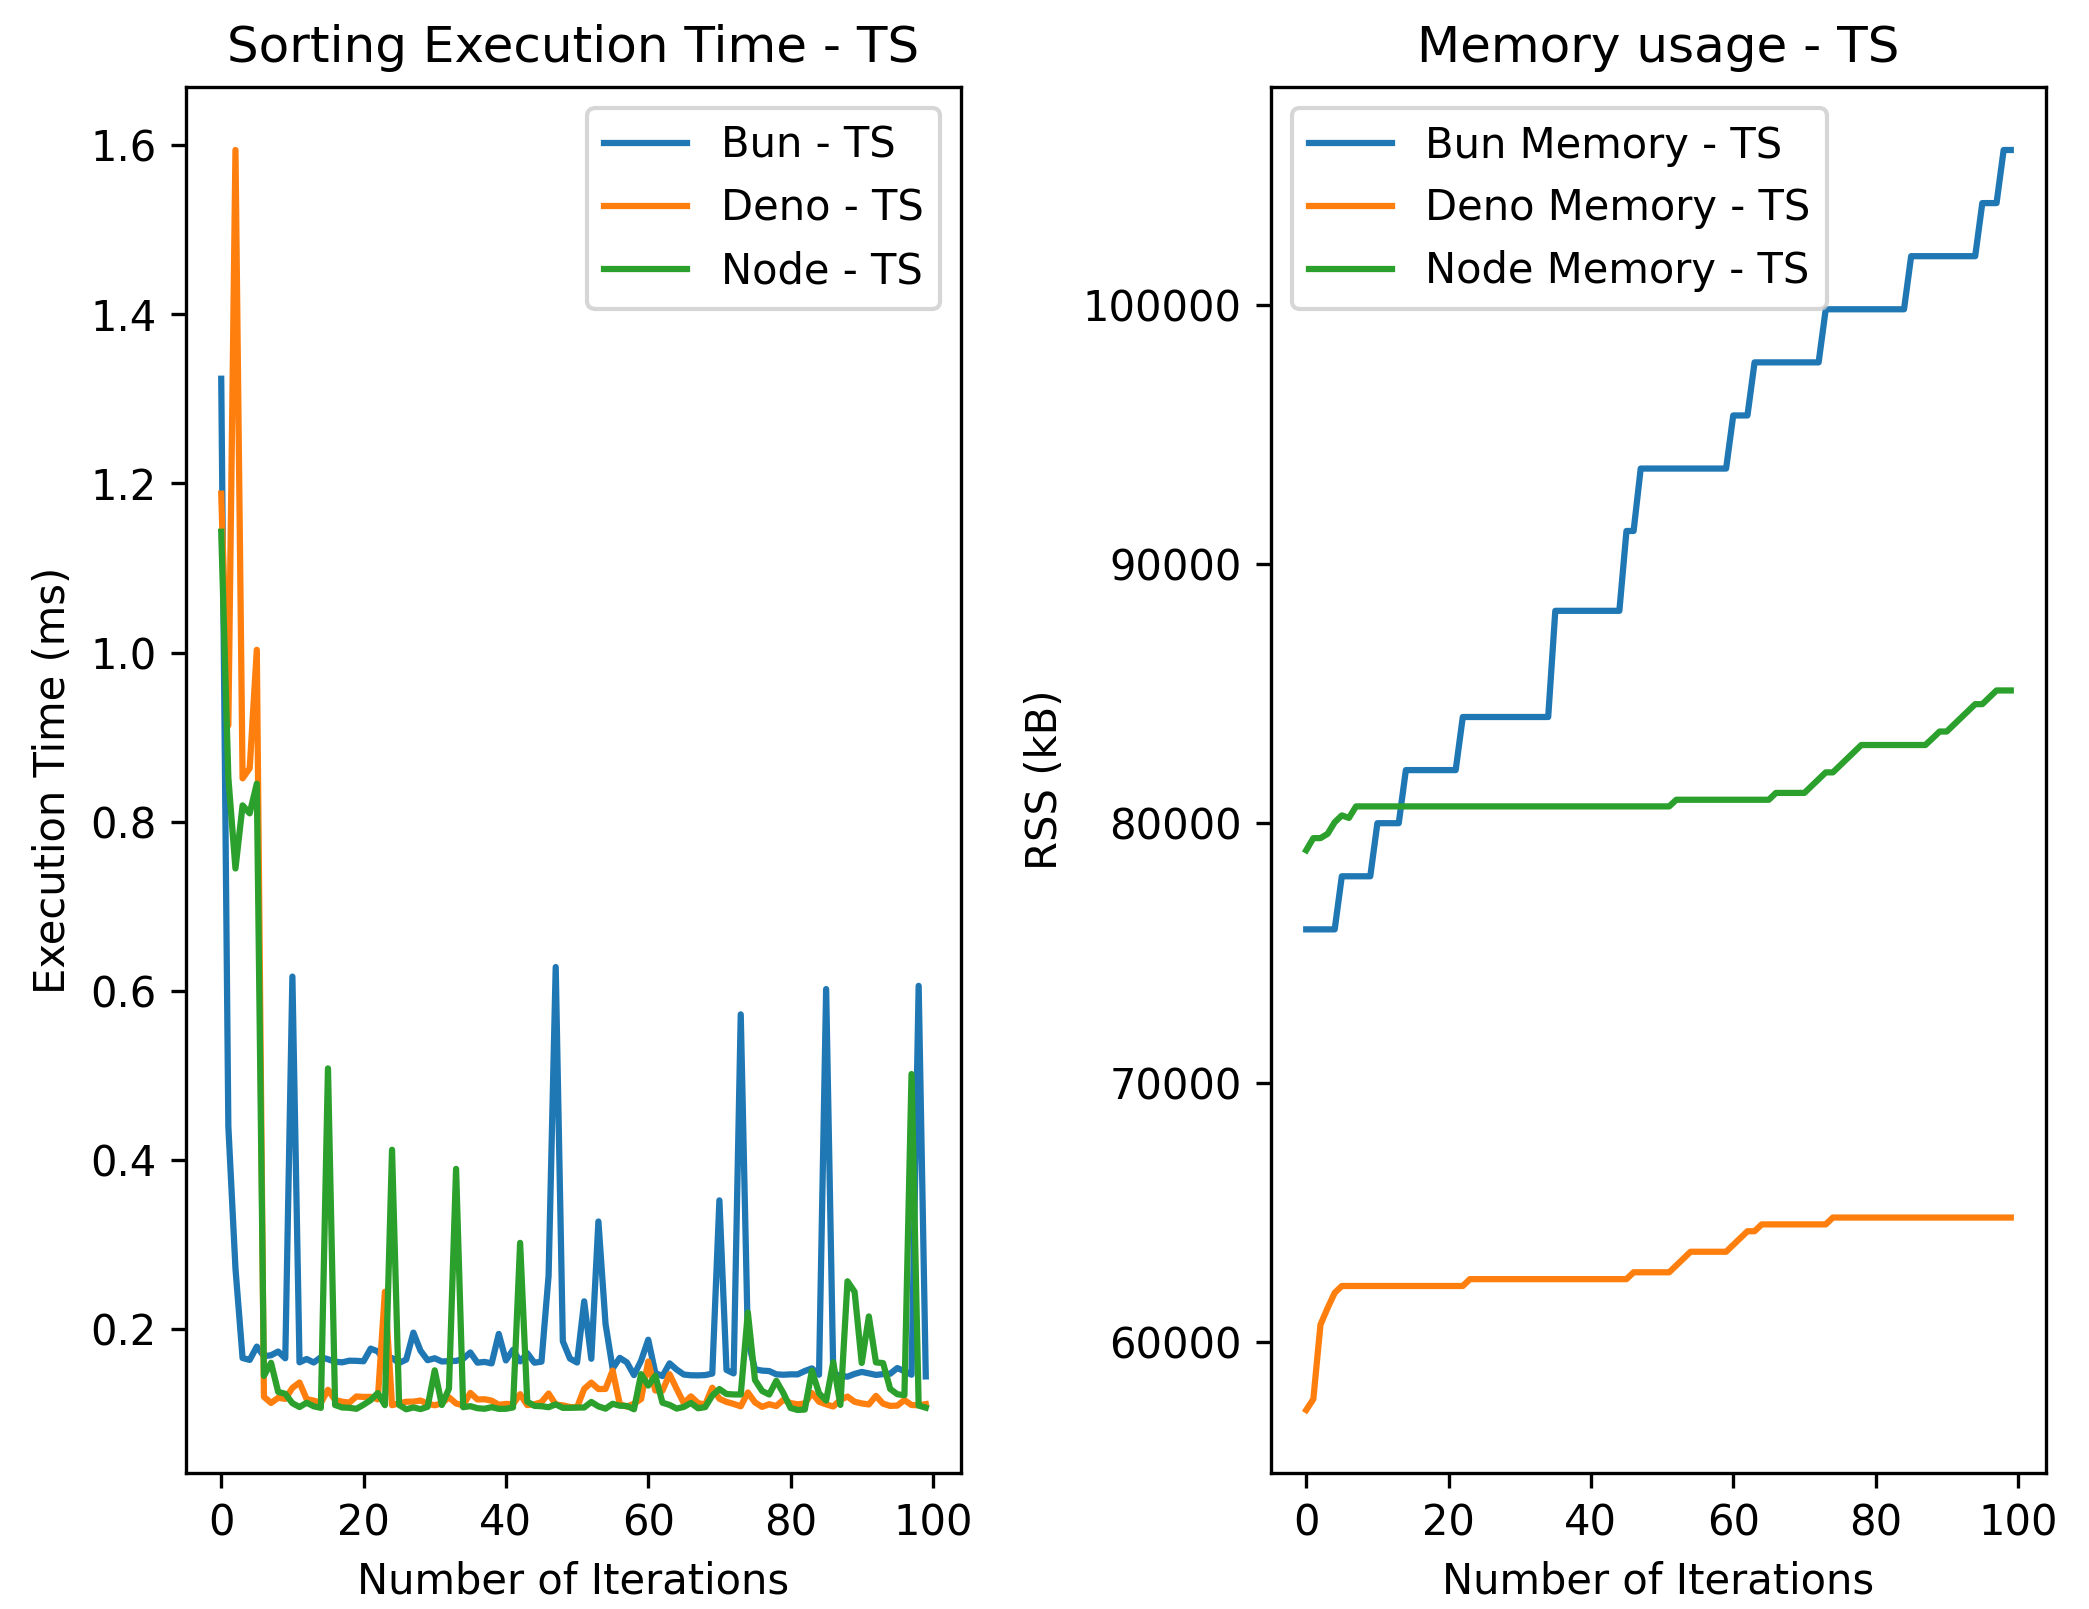
\includegraphics[width=0.7\textwidth]{Figures/sorting/sorting_radix_100_1000_ts.png}
  \caption{Wyniki eksperymentów dla algorytmu sortowania  dla 100 iteracji i 1000 elementów - po lewej czas wykonania jednorazowego testu w milisekundach, po prawej ilość zajmowanej pamięci w kilobajtach (kB)}
  \label{fig:radix_sorting_e1_ts}
\end{figure}

Na rysunku \ref{fig:radix_sorting_e2} przedstawiono wyniki eksperymentów dla algorytmu sortowania  dla 100 iteracji i 1000 elementów napisanego w języku JavaScript. Na wykresie przedstawiono czas wykonania jednorazowego testu w milisekundach oraz ilość zajmowanej pamięci w kilobajtach (kB).

\begin{figure}[H]
  \centering
  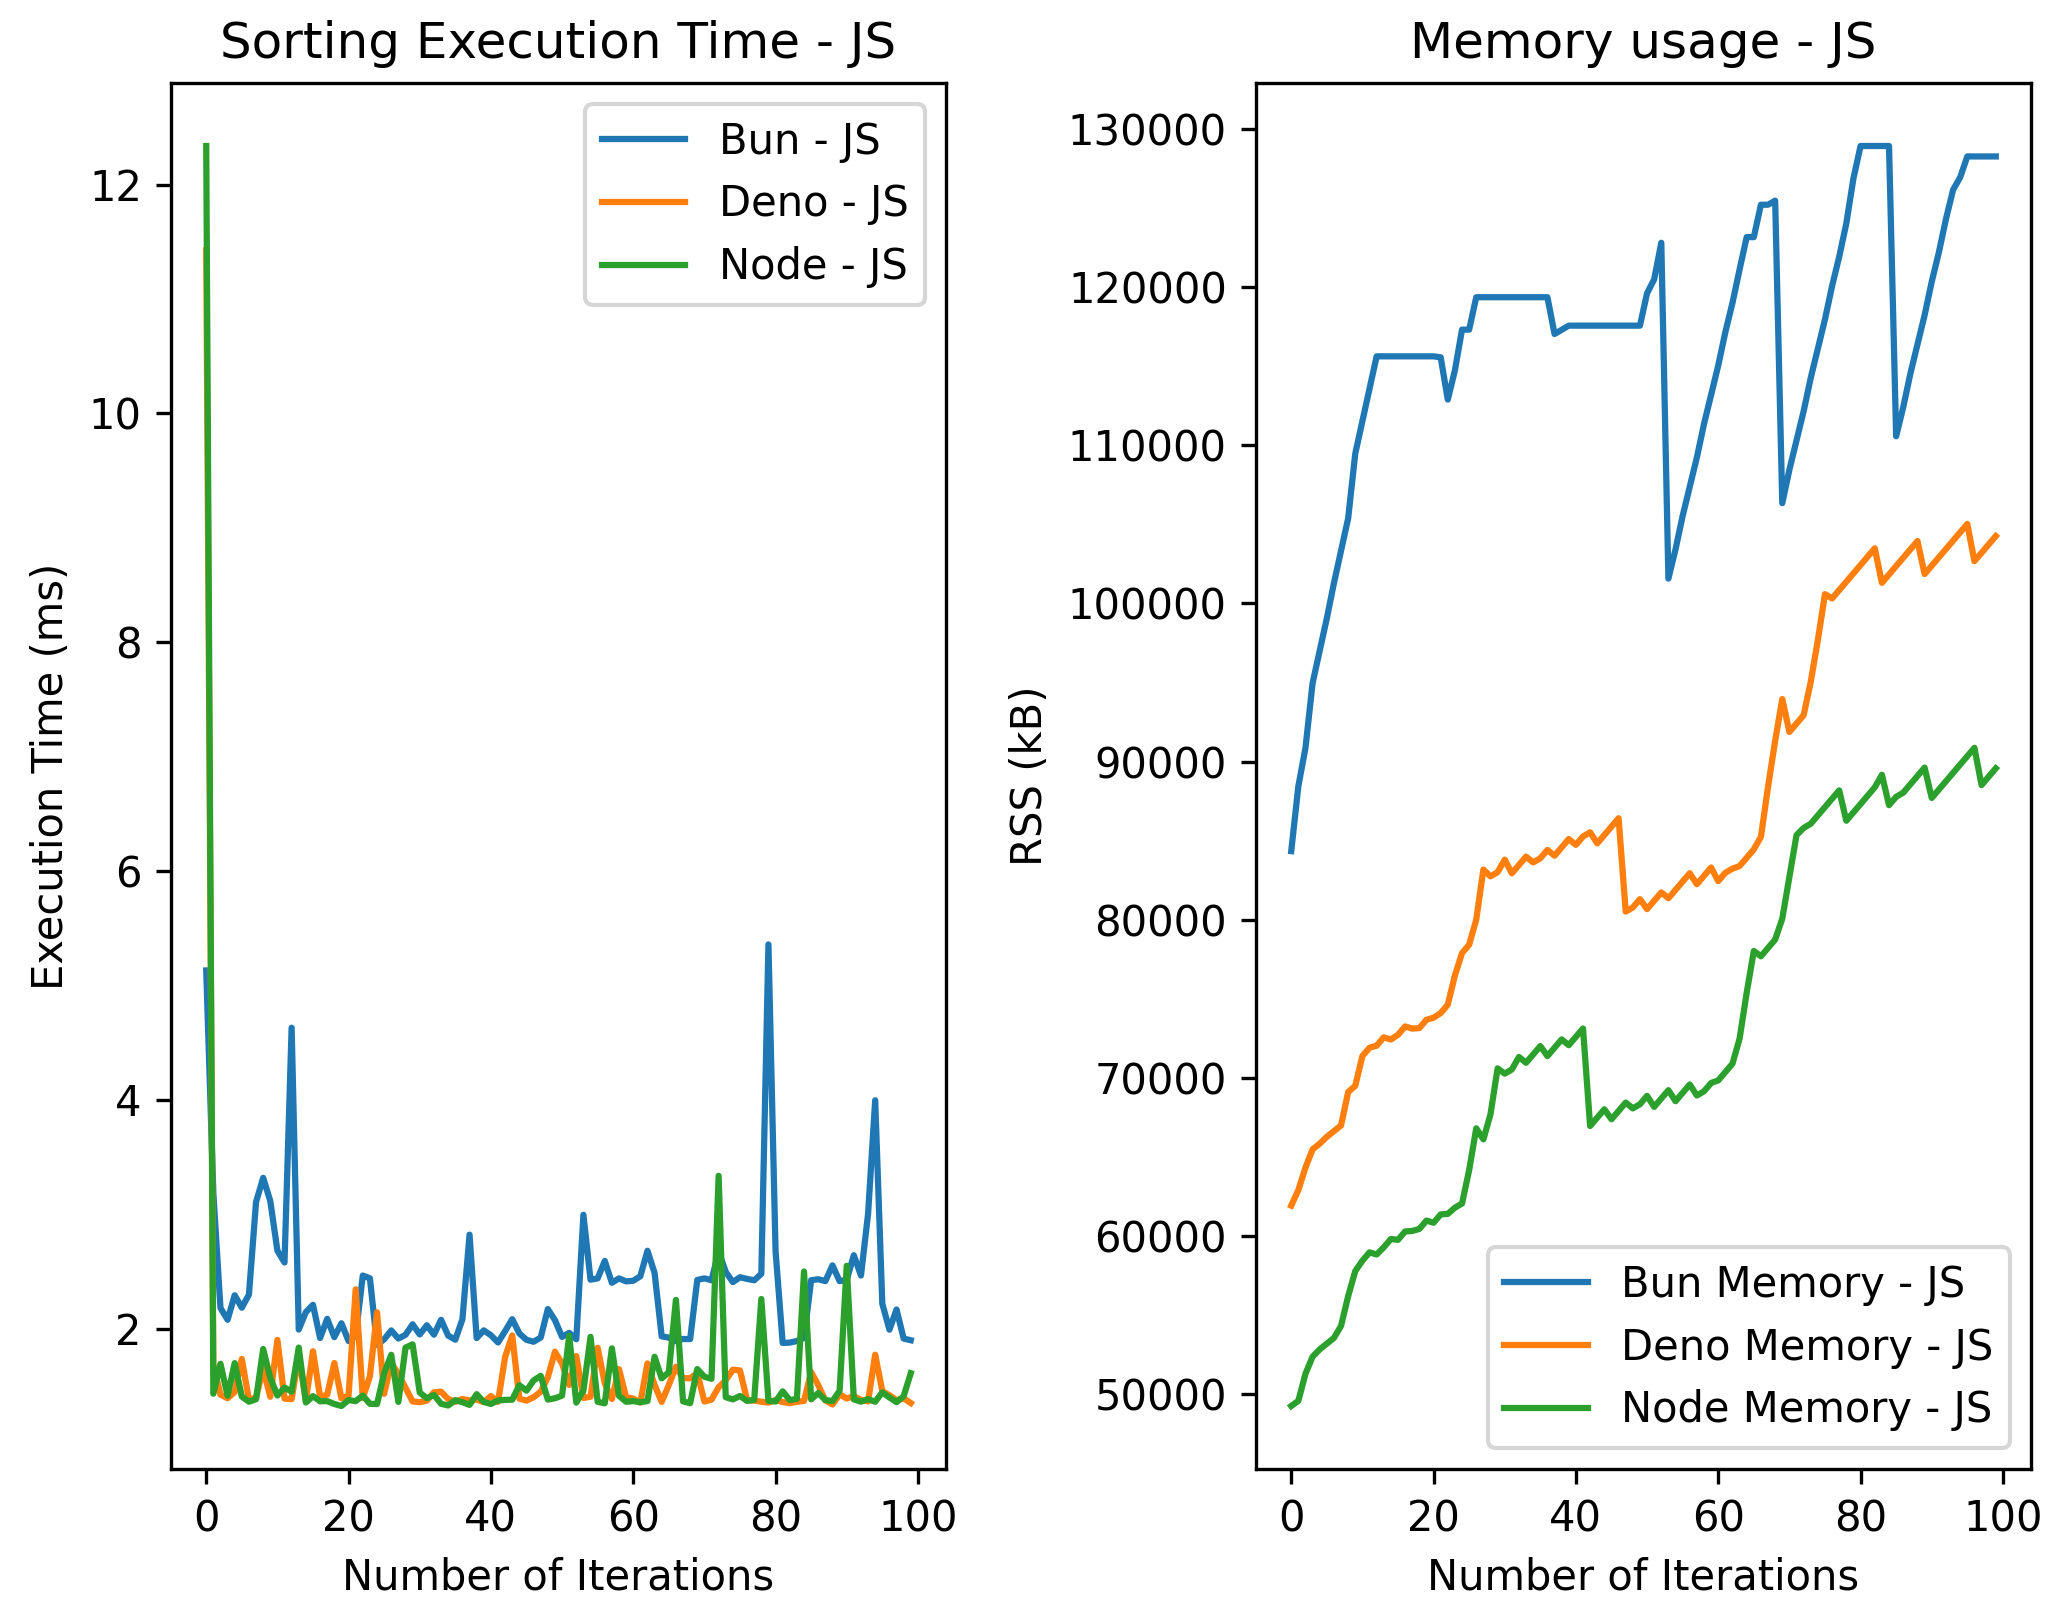
\includegraphics[width=0.7\textwidth]{Figures/sorting/sorting_radix_100_10000_js.png}
  \caption{Wyniki eksperymentów dla algorytmu sortowania  dla 100 iteracji i 10000 elementów - po lewej czas wykonania jednorazowego testu w milisekundach, po prawej ilość zajmowanej pamięci w kilobajtach (kB)}
  \label{fig:radix_sorting_e2}
\end{figure}

Na rysunku \ref{fig:radix_sorting_e2_ts} przedstawiono wyniki eksperymentów dla algorytmu sortowania  dla 100 iteracji i 10000 elementów napisanego w języku TypeScript. Na wykresie przedstawiono czas wykonania jednorazowego testu w milisekundach oraz ilość zajmowanej pamięci w kilobajtach (kB).

\begin{figure}[H]
  \centering
  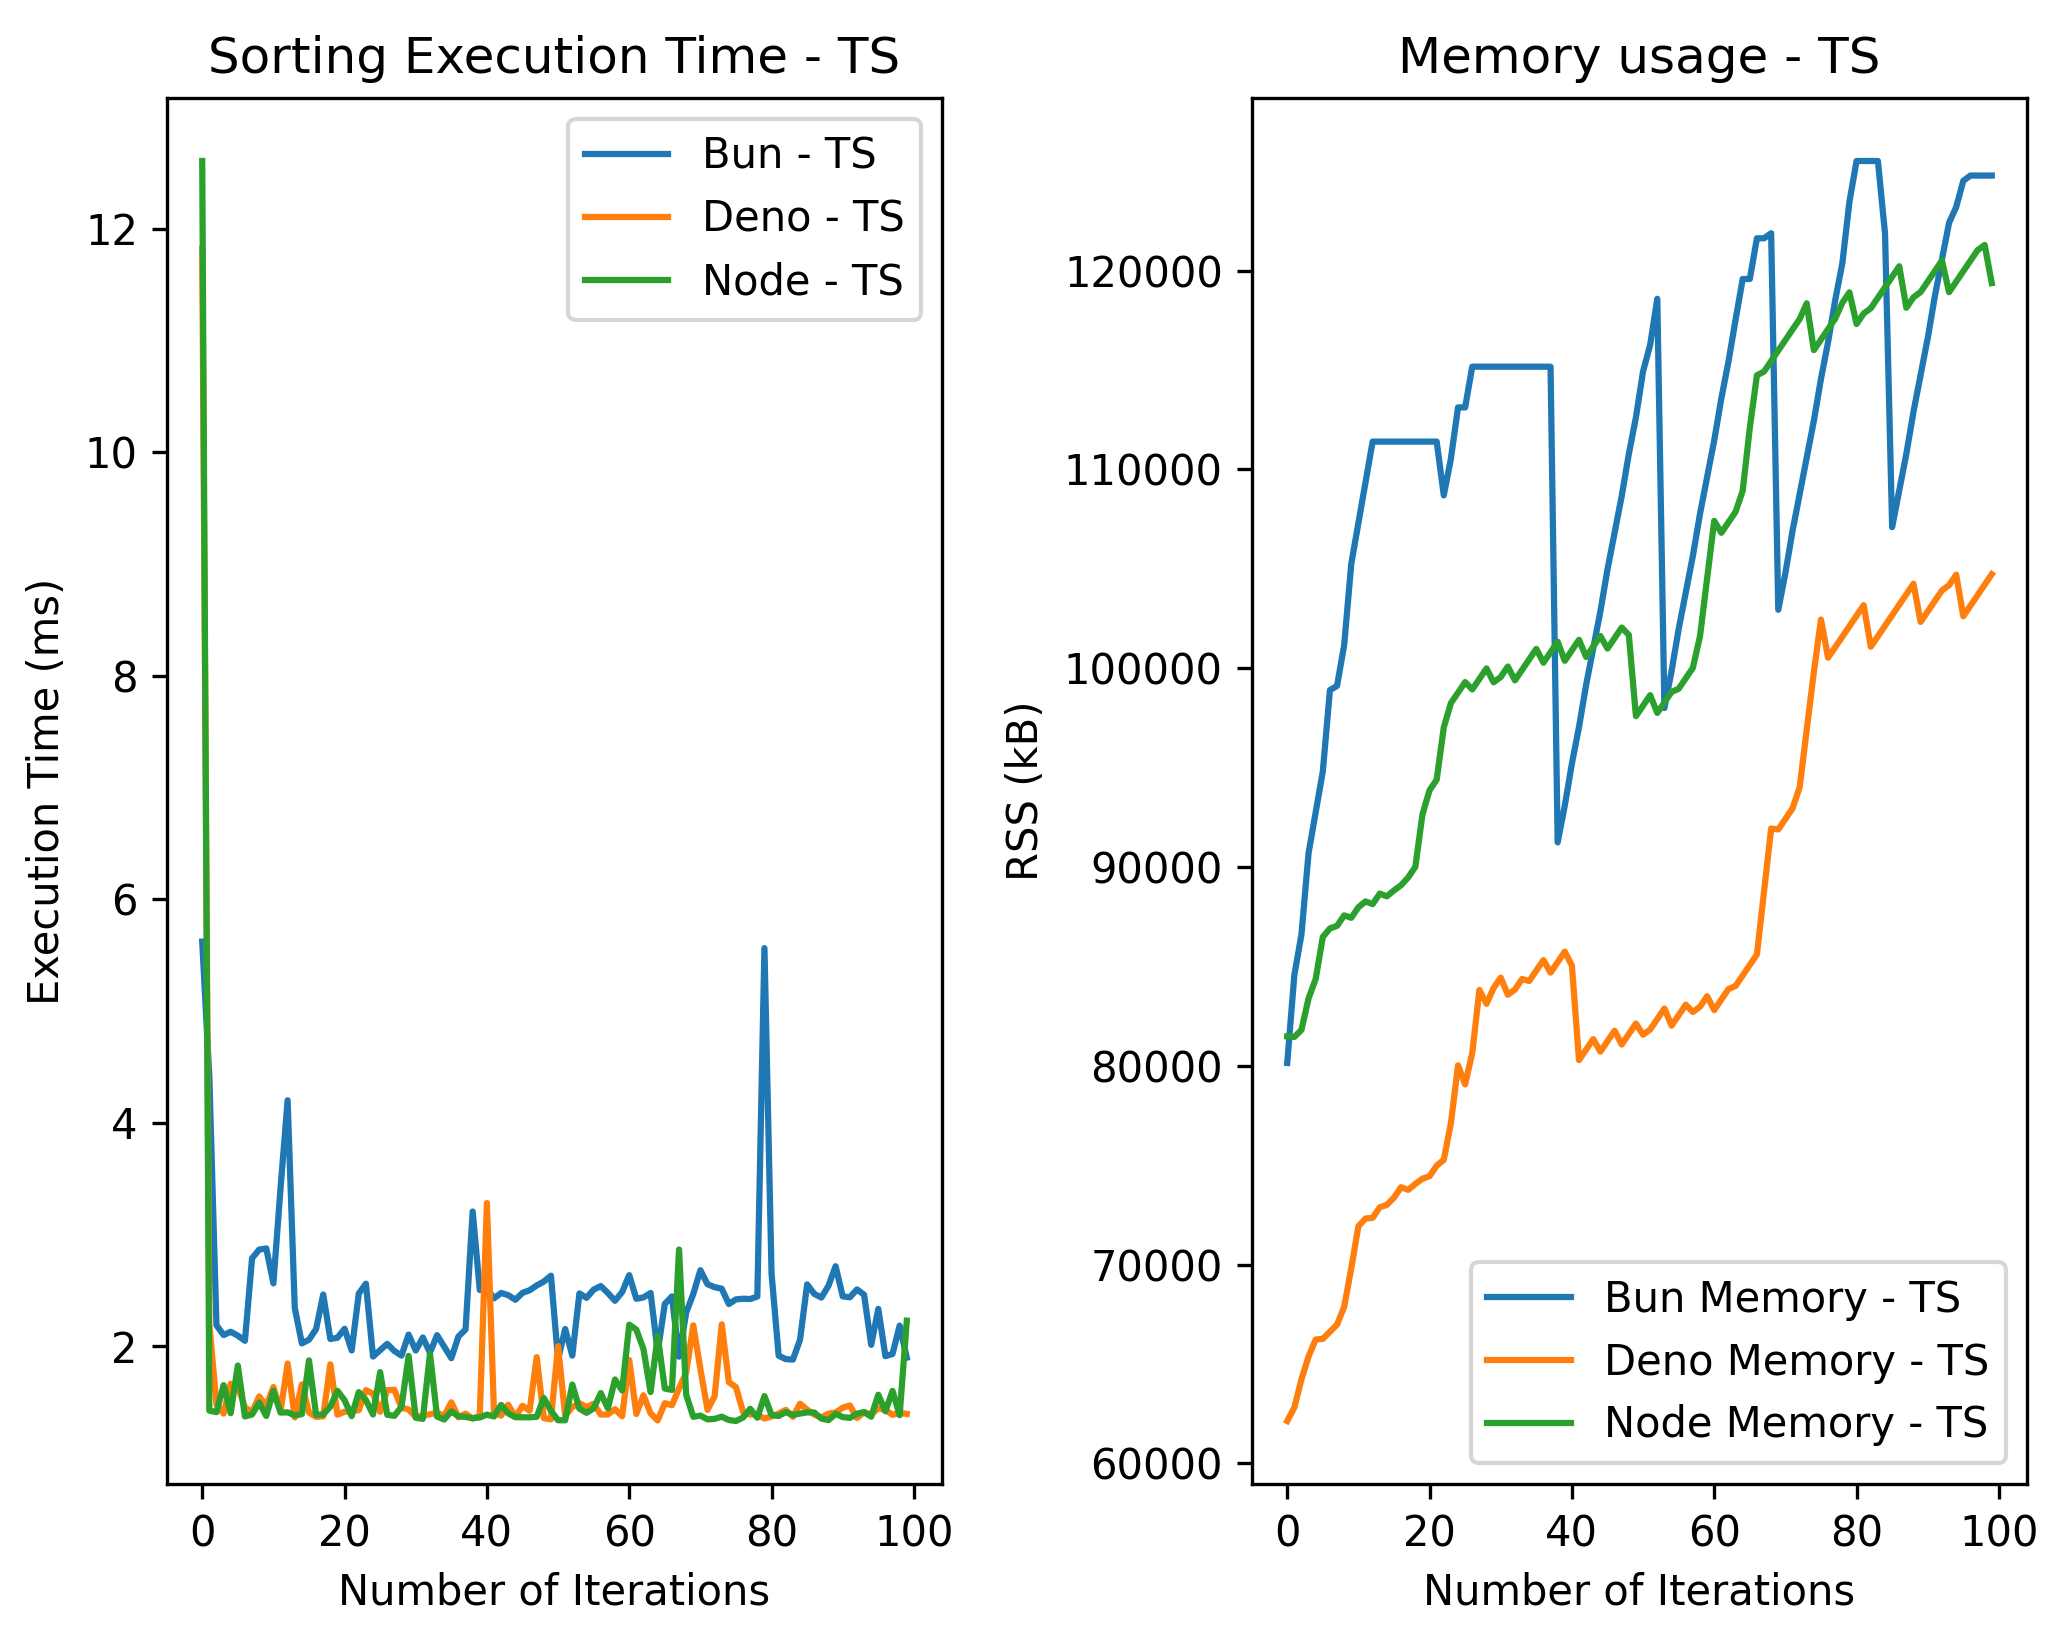
\includegraphics[width=0.7\textwidth]{Figures/sorting/sorting_radix_100_10000_ts.png}
  \caption{Wyniki eksperymentów dla algorytmu sortowania  dla 100 iteracji i 10000 elementów - po lewej czas wykonania jednorazowego testu w milisekundach, po prawej ilość zajmowanej pamięci w kilobajtach (kB)}
  \label{fig:radix_sorting_e2_ts}
\end{figure}

Na rysunku \ref{fig:radix_sorting_e3} przedstawiono wyniki eksperymentów dla algorytmu sortowania  dla 1000 iteracji i 1000 elementów napisanego w języku JavaScript. Na wykresie przedstawiono czas wykonania jednorazowego testu w milisekundach oraz ilość zajmowanej pamięci w kilobajtach (kB).

\begin{figure}[H]
  \centering
  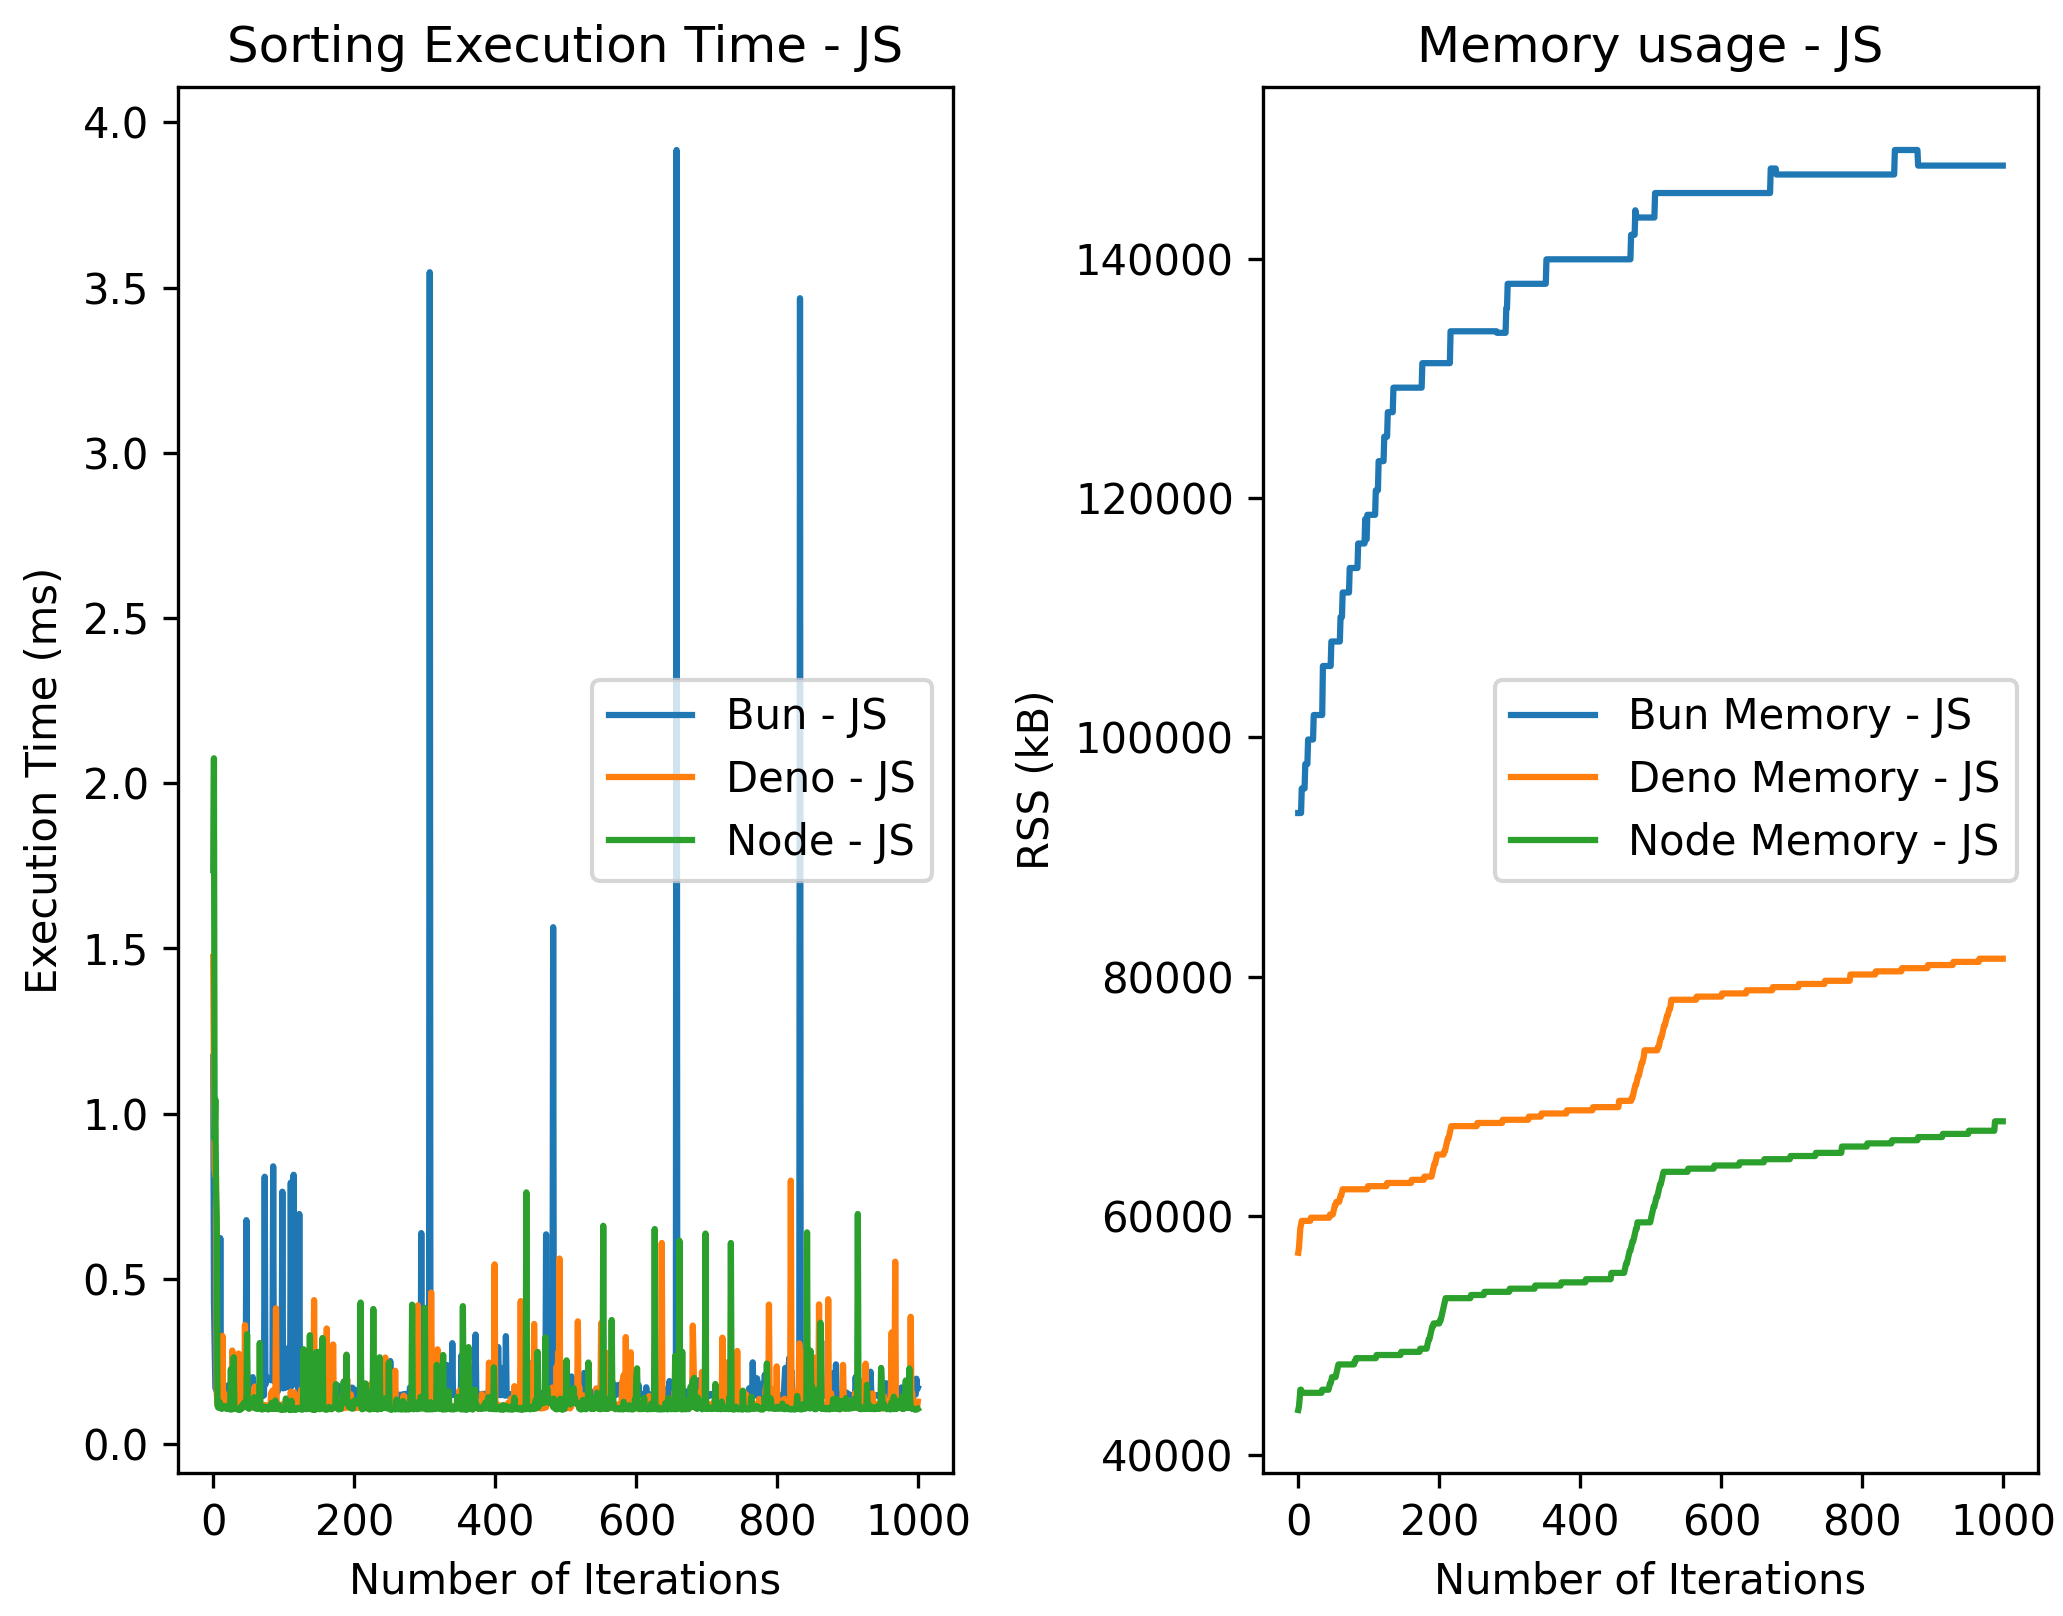
\includegraphics[width=0.7\textwidth]{Figures/sorting/sorting_radix_1000_1000_js.png}
  \caption{Wyniki eksperymentów dla algorytmu sortowania  dla 1000 iteracji i 1000 elementów - po lewej czas wykonania jednorazowego testu w milisekundach, po prawej ilość zajmowanej pamięci w kilobajtach (kB)}
  \label{fig:radix_sorting_e3}
\end{figure}

Na rysunku \ref{fig:radix_sorting_e3_ts} przedstawiono wyniki eksperymentów dla algorytmu sortowania  dla 1000 iteracji i 1000 elementów napisanego w języku TypeScript. Na wykresie przedstawiono czas wykonania jednorazowego testu w milisekundach oraz ilość zajmowanej pamięci w kilobajtach (kB).

\begin{figure}[H]
  \centering
  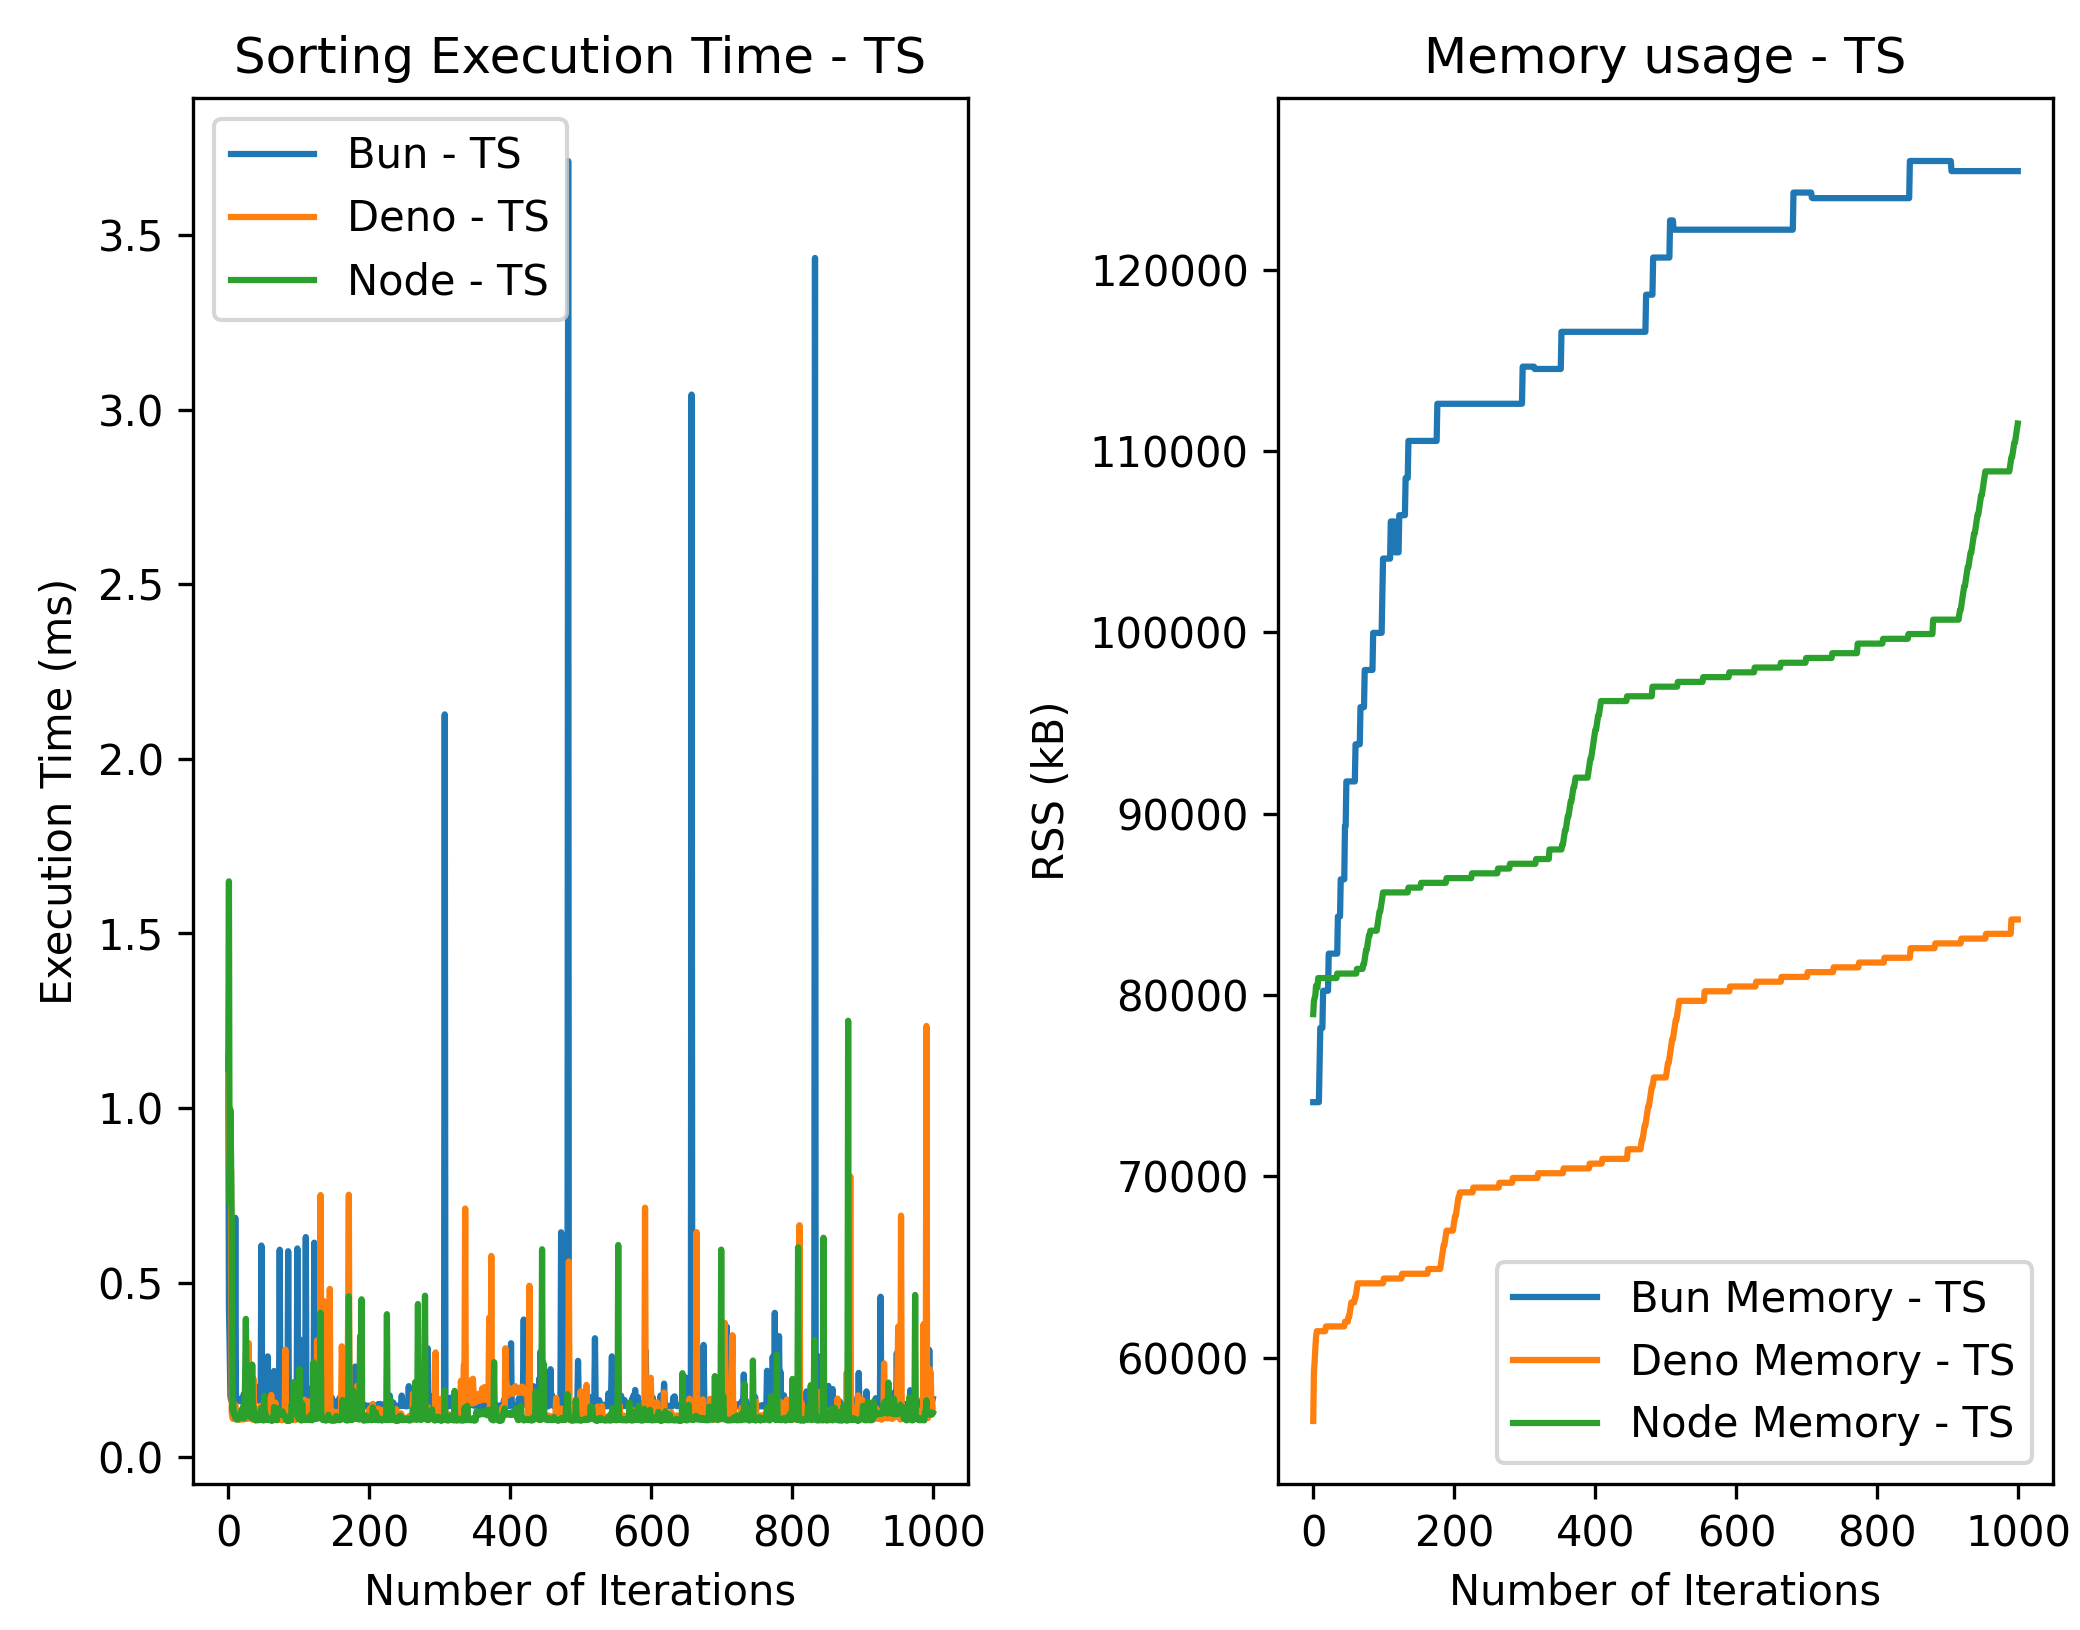
\includegraphics[width=0.7\textwidth]{Figures/sorting/sorting_radix_1000_1000_ts.png}
  \caption{Wyniki eksperymentów dla algorytmu sortowania  dla 1000 iteracji i 1000 elementów - po lewej czas wykonania jednorazowego testu w milisekundach, po prawej ilość zajmowanej pamięci w kilobajtach (kB)}
  \label{fig:radix_sorting_e3_ts}
\end{figure}

Na rysunku \ref{fig:radix_sorting_e4} przedstawiono wyniki eksperymentów dla algorytmu sortowania  dla 100 iteracji i 1000 elementów napisanego w języku JavaScript. Na wykresie przedstawiono czas wykonania jednorazowego testu w milisekundach oraz ilość zajmowanej pamięci w kilobajtach (kB).

\begin{figure}[H]
  \centering
  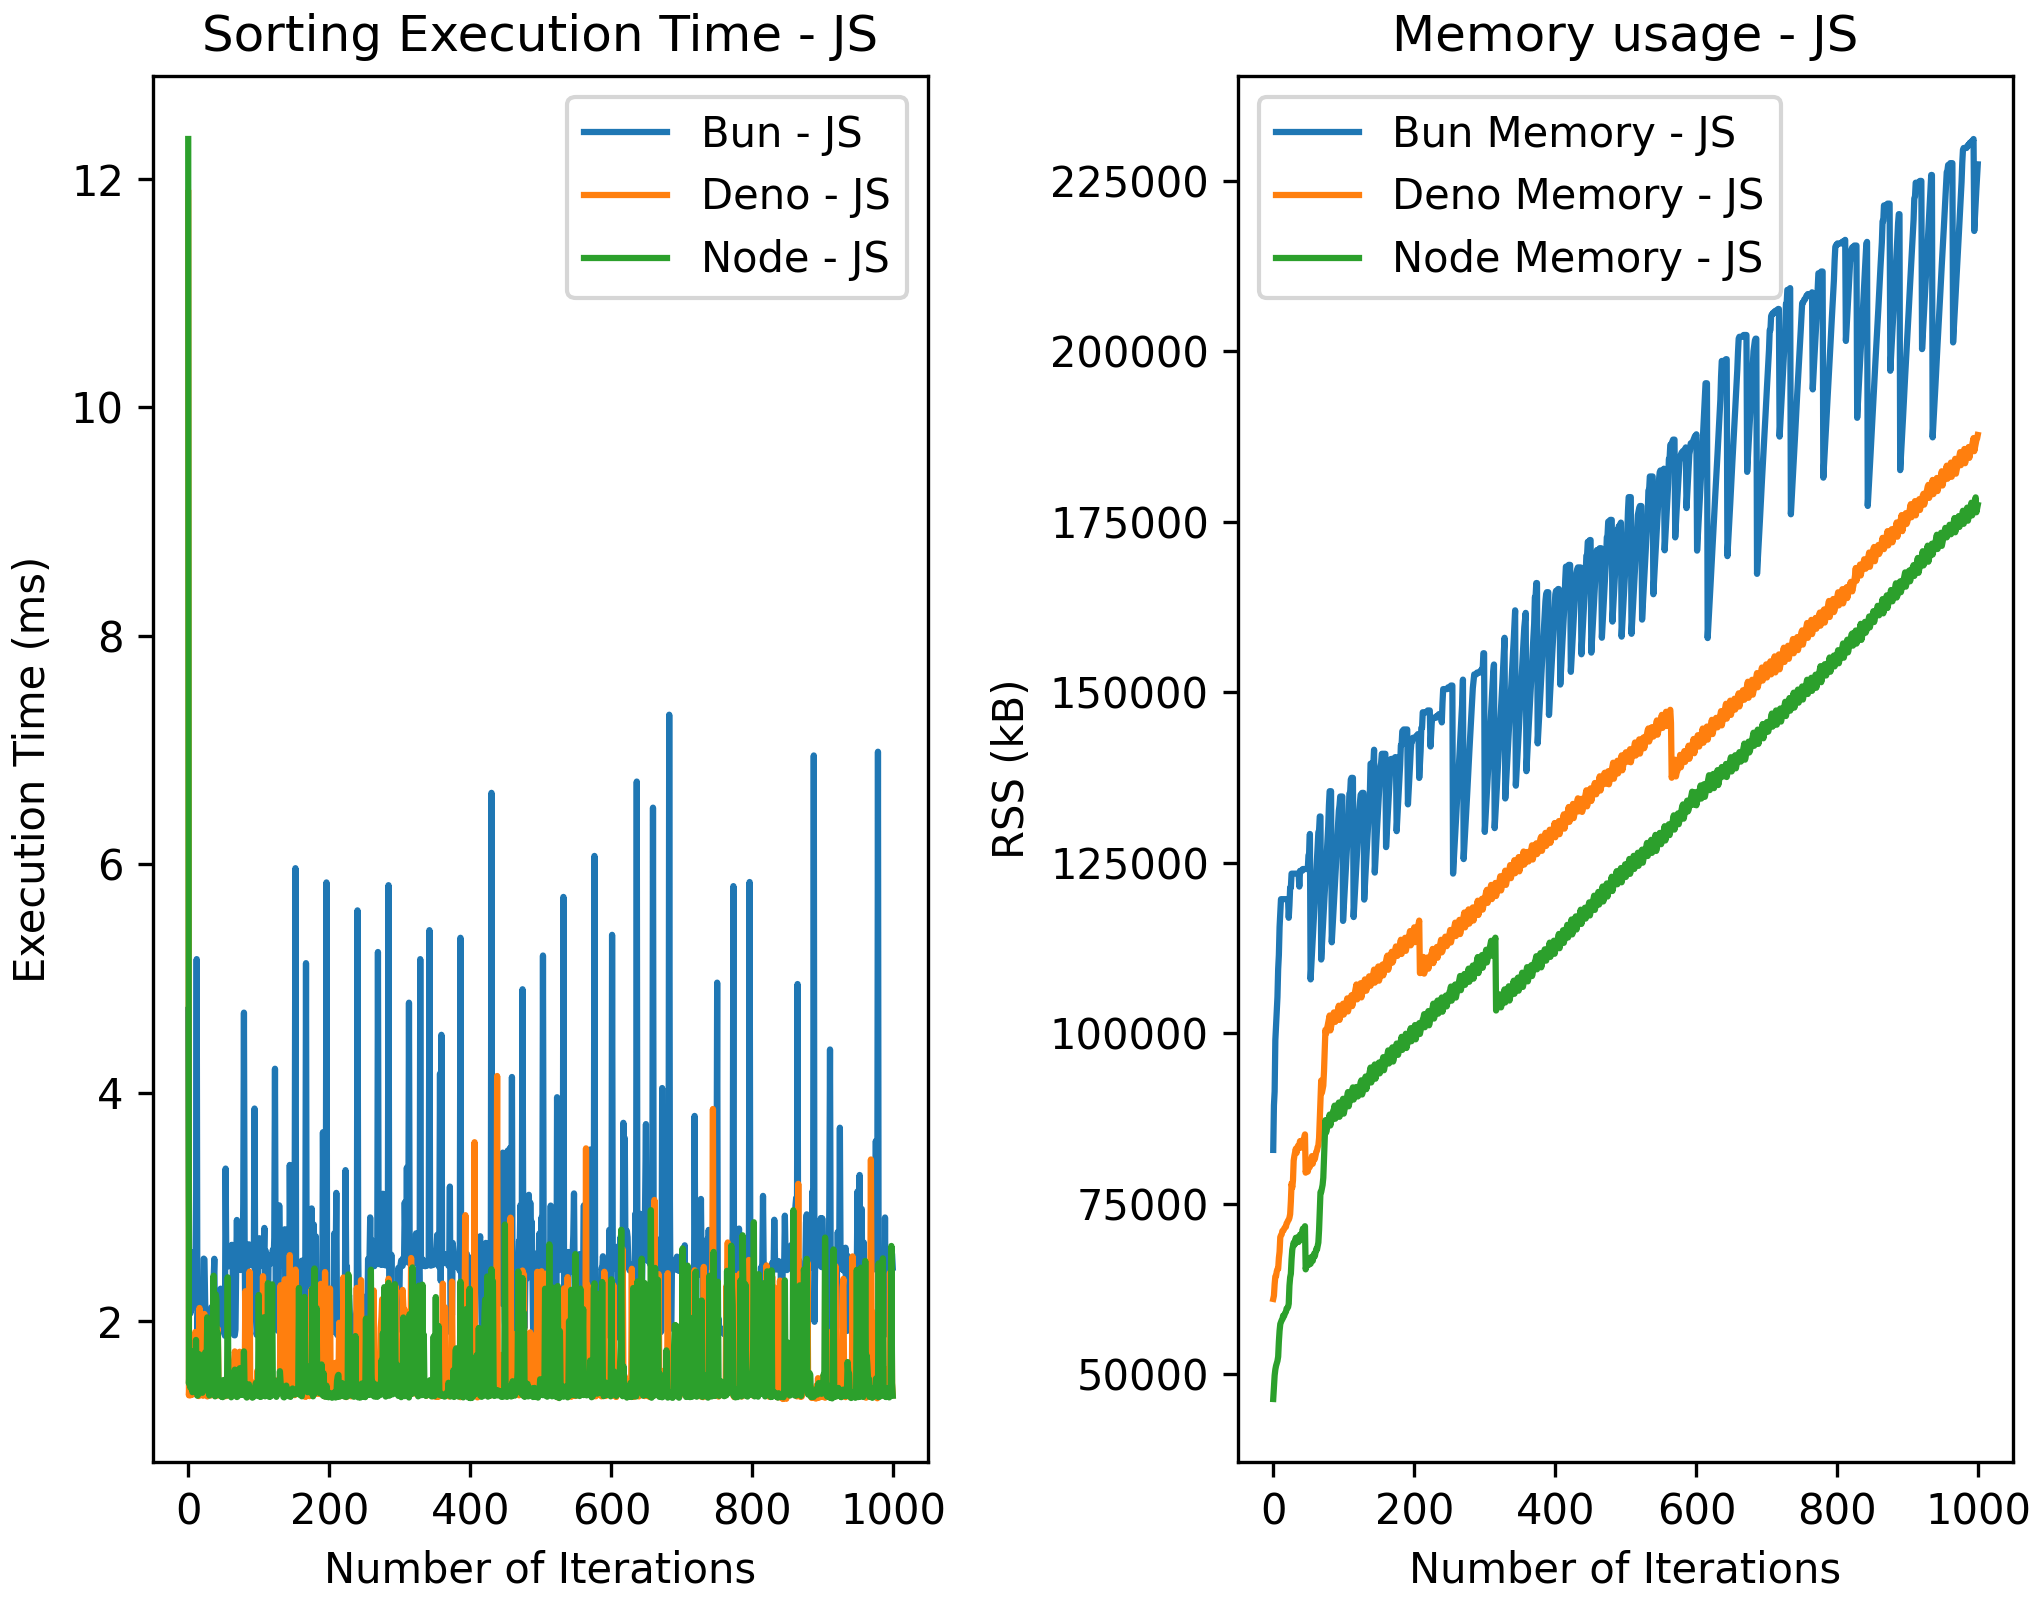
\includegraphics[width=0.7\textwidth]{Figures/sorting/sorting_radix_1000_10000_js.png}
  \caption{Wyniki eksperymentów dla algorytmu sortowania  dla 1000 iteracji i 10000 elementów - po lewej czas wykonania jednorazowego testu w milisekundach, po prawej ilość zajmowanej pamięci w kilobajtach (kB)}
  \label{fig:radix_sorting_e4}
\end{figure}

Na rysunku \ref{fig:radix_sorting_e4_ts} przedstawiono wyniki eksperymentów dla algorytmu sortowania pozycyjnego dla 1000 iteracji i 10000 elementów napisanego w języku TypeScript. Na wykresie przedstawiono czas wykonania jednorazowego testu w milisekundach oraz ilość zajmowanej pamięci w kilobajtach (kB).

\begin{figure}[H]
  \centering
  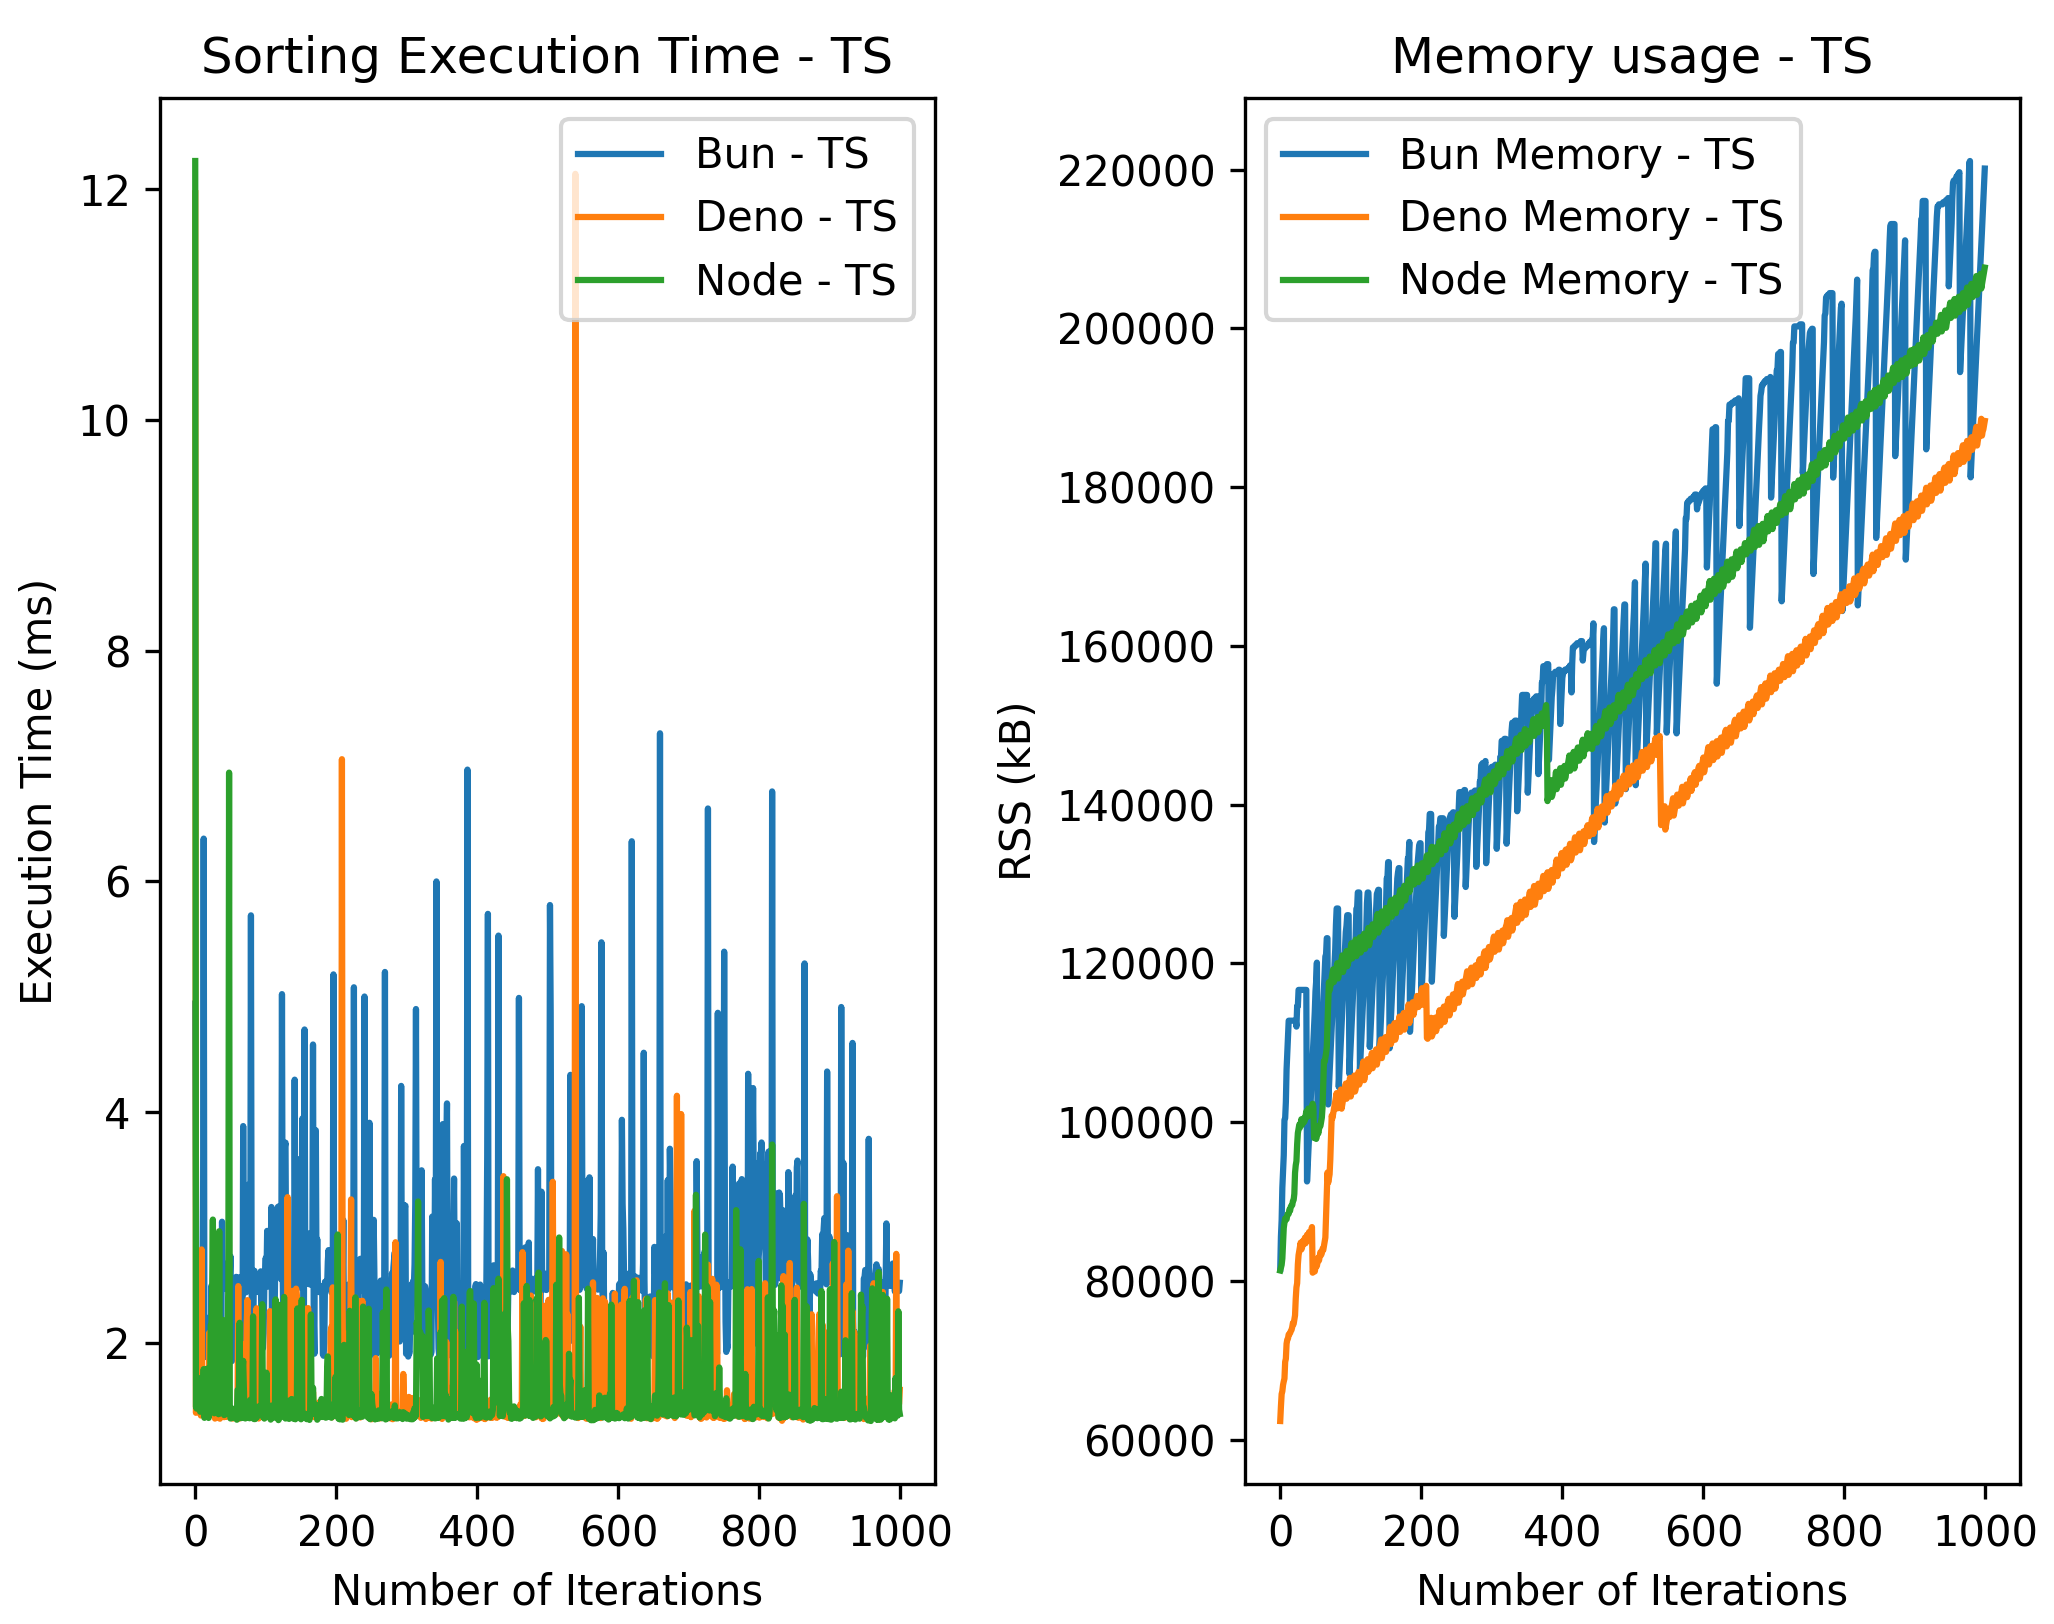
\includegraphics[width=0.7\textwidth]{Figures/sorting/sorting_radix_1000_10000_ts.png}
  \caption{Wyniki eksperymentów dla algorytmu sortowania  dla 100 iteracji i 10000 elementów - po lewej czas wykonania jednorazowego testu w milisekundach, po prawej ilość zajmowanej pamięci w kilobajtach (kB)}
  \label{fig:radix_sorting_e4_ts}
\end{figure}

\subsection{Algorytmy kodowania}
W celu zbadania wydajności możliwości kodowania dla środowisk, użyto algorytmu kodowania Base64, który jest najpopularniejszym algorytmem kodowania wykorzystywanym w aplikacjach webowych. W tabeli \ref{tab:encoding_experiments} przedstawiono liczbę przeprowadzonych eksperymentów, długość kodowanego słowa.

\begin{table}[H]
  \centering
  \caption{Parametry eksperymentów algorytmu kodowania Base64}
  \begin{tabular}{|c|c|}
    \hline
    \textbf{Liczba eksperymentów} & \textbf{Długość słowa}\\ \hline
    1000 & 8192 \\ \hline
    100 & 32768 \\ \hline
  \end{tabular}
  \label{tab:encoding_experiments}
\end{table}

\subsubsection{Wyniki}

\subsection{Testy wydajnościowe operacji zapisu i odczytu plików}
W celu zbadania wydajności operacji zapisu oraz odczytu plików, przeprowadzono eksperymenty, które polegały na zapisie oraz odczycie plików o różnych rozmiarach. W przeprowadzonych testach wykorzystano pliki tekstowe. Do wypełnienia plików przykładowym tekstem. Zawartość plików została wygenerowana za pomocą modułu \textit{faker.js}. W tabeli \ref{tab:file_experiments} przedstawiono liczbę przeprowadzonych eksperymentów oraz rozmiar pliku.

\begin{table}[H]
  \centering
  \caption{Parametry eksperymentów zapisu i odczytu plików}
  \begin{tabular}{|c|c|c|}
    \hline
    \textbf{Ilość eksperymentów} & \textbf{Rozmiar pliku} & \textbf{Ilość plików} \\ \hline
    50 & 512kB & 50 \\ \hline
    50 & 1MB & 50 \\ \hline
  \end{tabular}
  \label{tab:file_experiments}
\end{table}

\subsubsection{Wyniki}

\subsection{Testy wydajnościowe serwera HTTP}
W celu zbadania wydajności serwera HTTP, przeprowadzono testy obciążeniowe. Do testów została wykorzystany program \textit{oha} \cite{oha}, który pozwala na połączenie się do serwera HTTP oraz wysyłanie żądań z kilku połączeń jednocześnie. W tabeli \ref{tab:http_experiments} przedstawiono liczbę przeprowadzonych eksperymentów oraz ilość połączeń.

\begin{table}[H]
  \centering
  \caption{Parametry eksperymentów serwera HTTP}
  \begin{tabular}{|c|c|}
    \hline
    \textbf{Liczba żądań} & \textbf{Ilość połączeń}\\ \hline
    10000 & 100 \\ \hline
    10000 & 1000 \\ \hline
    10000 & 10000 \\ \hline
  \end{tabular}
  \label{tab:http_experiments}
\end{table}

\subsubsection{Wyniki}

\subsection{Testy wydajnościowe zapisu i odczytu danych z bazy danych}
W celu zbadania wydajności operacji zapisu oraz odczytu danych z bazy danych, przeprowadzono testy wydajnościowe z wykorzystaniem bazy danych SQLite. W celu wygenerowania danych do bazy danych, wykorzystano moduł \textit{faker.js}. W tabeli \ref{tab:database_experiments} przedstawiono liczbę przeprowadzonych eksperymentów oraz ilość rekordów.

\begin{table}[H]
  \centering
  \caption{Parametry eksperymentów zapisu i odczytu danych z bazy danych}
  \begin{tabular}{|c|c|}
    \hline
    \textbf{Liczba eksperymentów} & \textbf{Ilość rekordów}\\ \hline
    10 & 1000 \\ \hline
    100 & 1000 \\ \hline
  \end{tabular}
  \label{tab:database_experiments}
\end{table}

\subsubsection{Wyniki}

\begin{figure}[H]
  \centering
  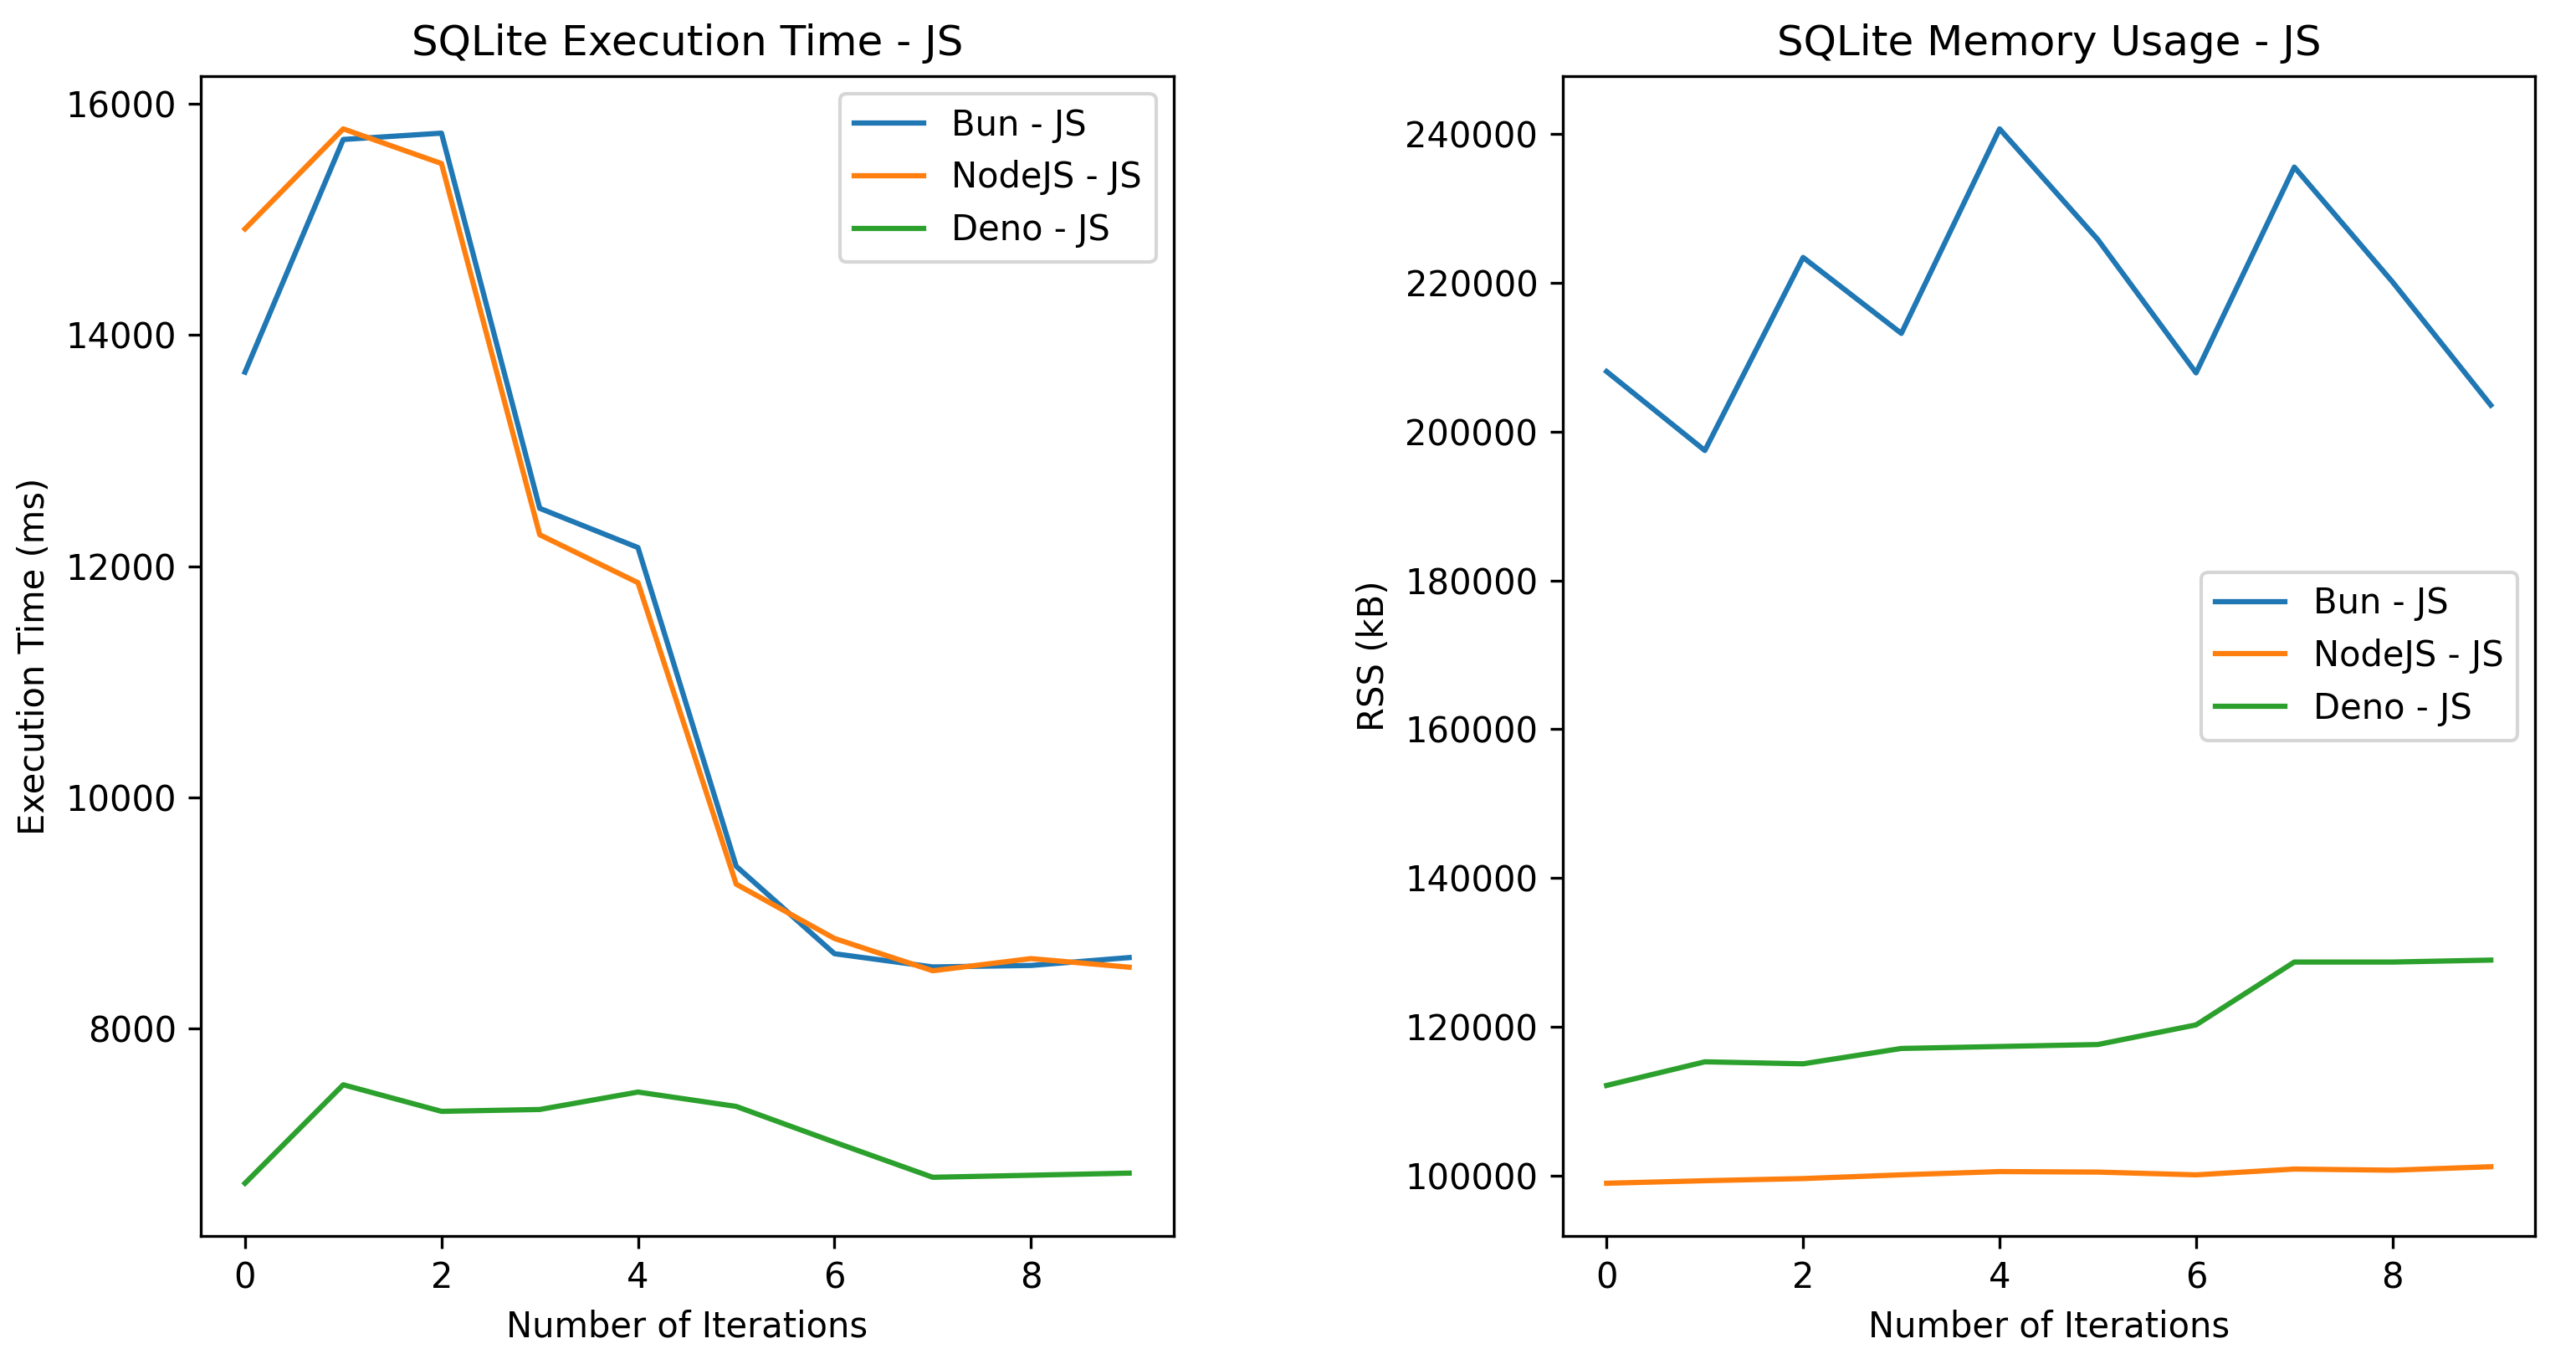
\includegraphics[width=0.7\textwidth]{Figures/database/sqlite_10_1000_js.png}
  \caption{Wyniki eksperymentów dla testu bazy danych 10 iteracji oraz 1000 rekordów - po lewej czas wykonania jednorazowego testu w milisekundach, po prawej ilość zajmowanej pamięci w kilobajtach (kB)}
  \label{fig:database_e1_js}
\end{figure}

\begin{figure}[H]
  \centering
  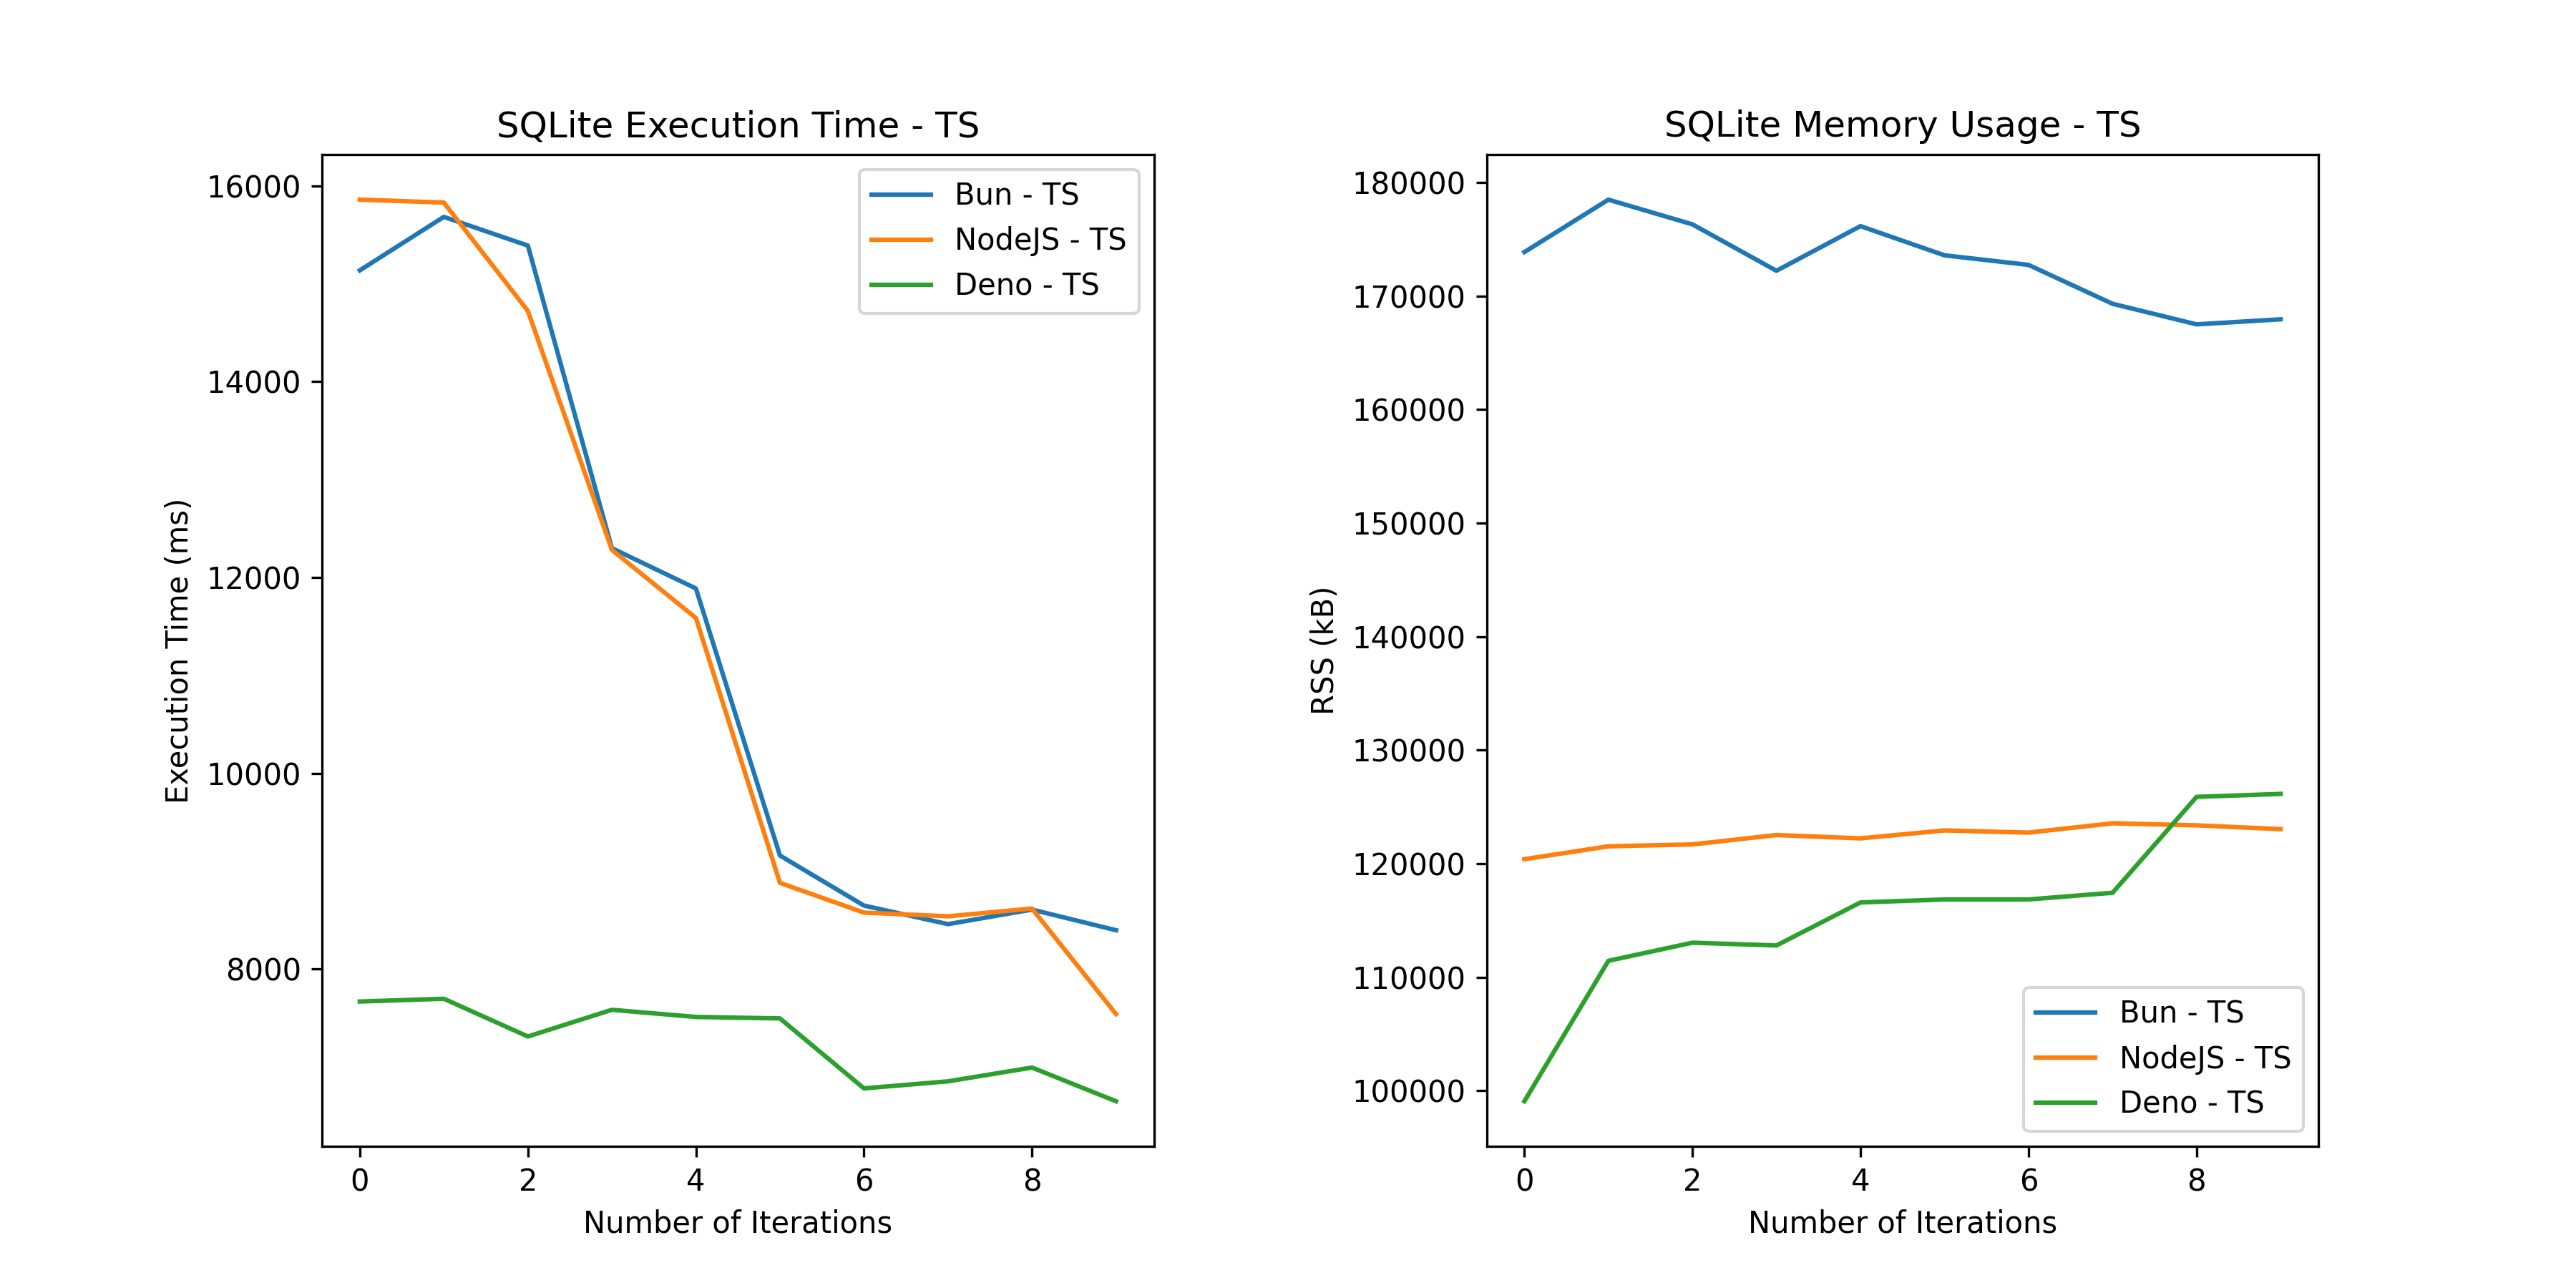
\includegraphics[width=0.7\textwidth]{Figures/database/sqlite_10_1000_ts.png}
  \caption{Wyniki eksperymentów dla testu bazy danych 10 iteracji oraz 1000 rekordów - po lewej czas wykonania jednorazowego testu w milisekundach, po prawej ilość zajmowanej pamięci w kilobajtach (kB)}
  \label{fig:database_e1_ts}
\end{figure}

\begin{figure}[H]
  \centering
  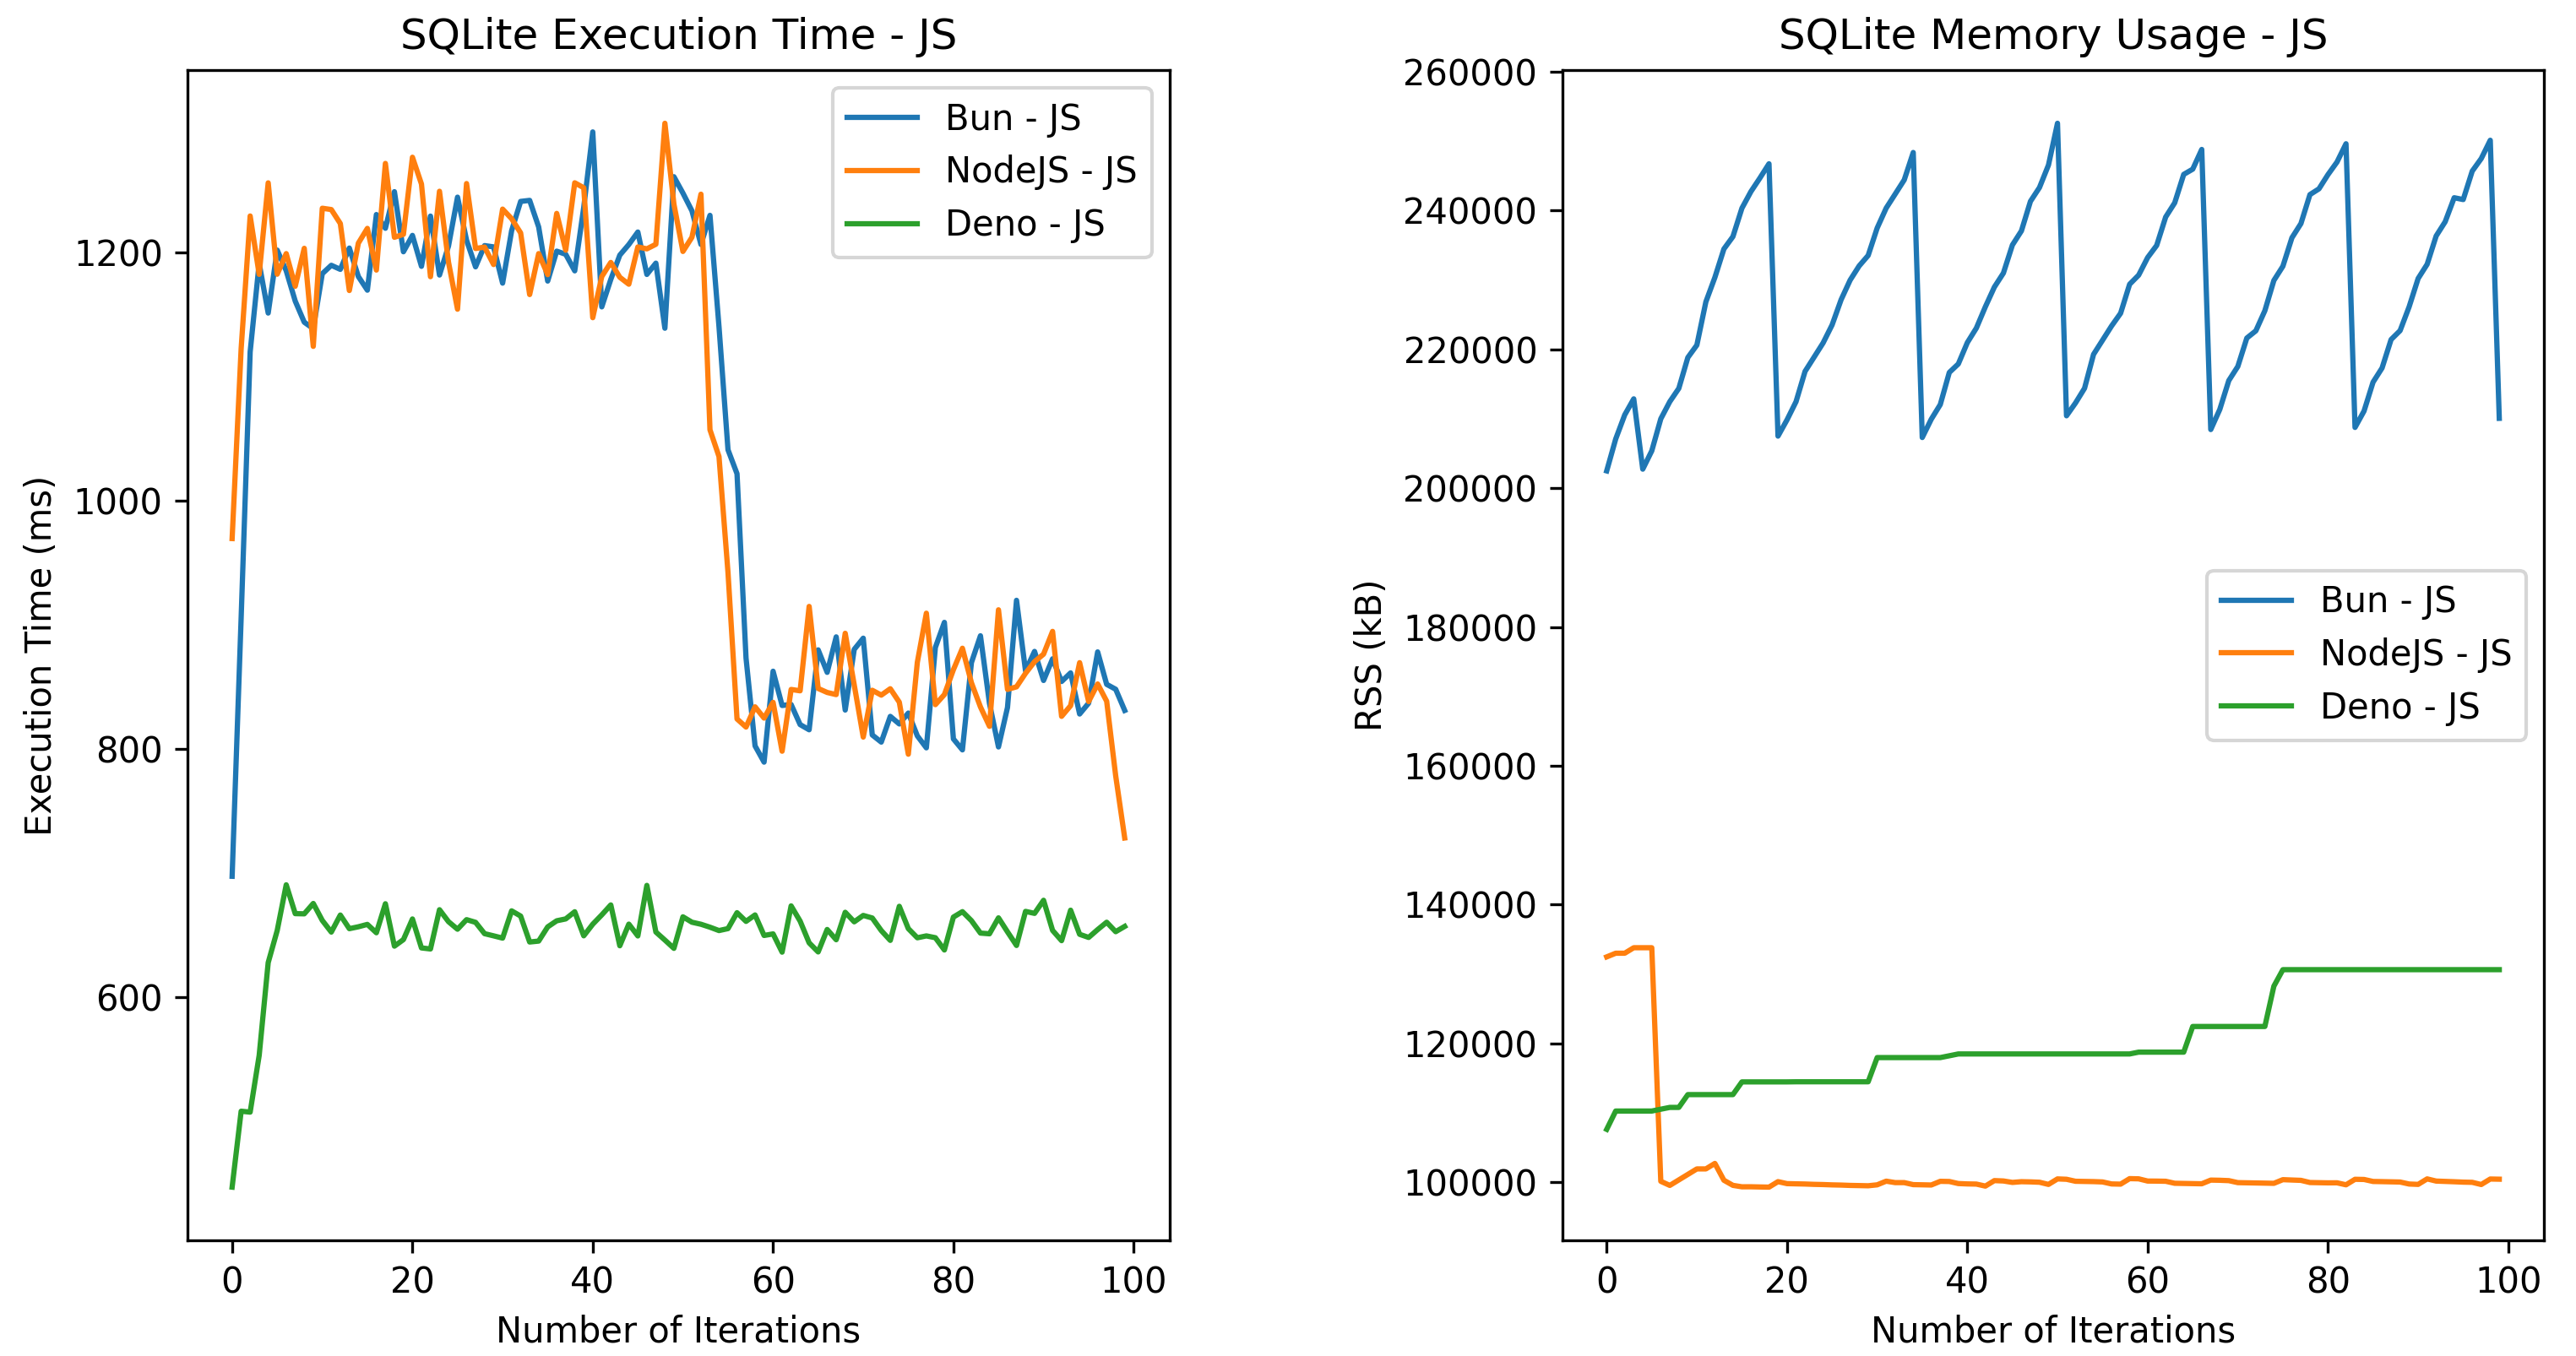
\includegraphics[width=0.7\textwidth]{Figures/database/sqlite_100_1000_js.png}
  \caption{Wyniki eksperymentów dla testu bazy danych 100 iteracji oraz 1000 rekordów - po lewej czas wykonania jednorazowego testu w milisekundach, po prawej ilość zajmowanej pamięci w kilobajtach (kB)}
  \label{fig:database_e2_js}
\end{figure}

\begin{figure}[H]
  \centering
  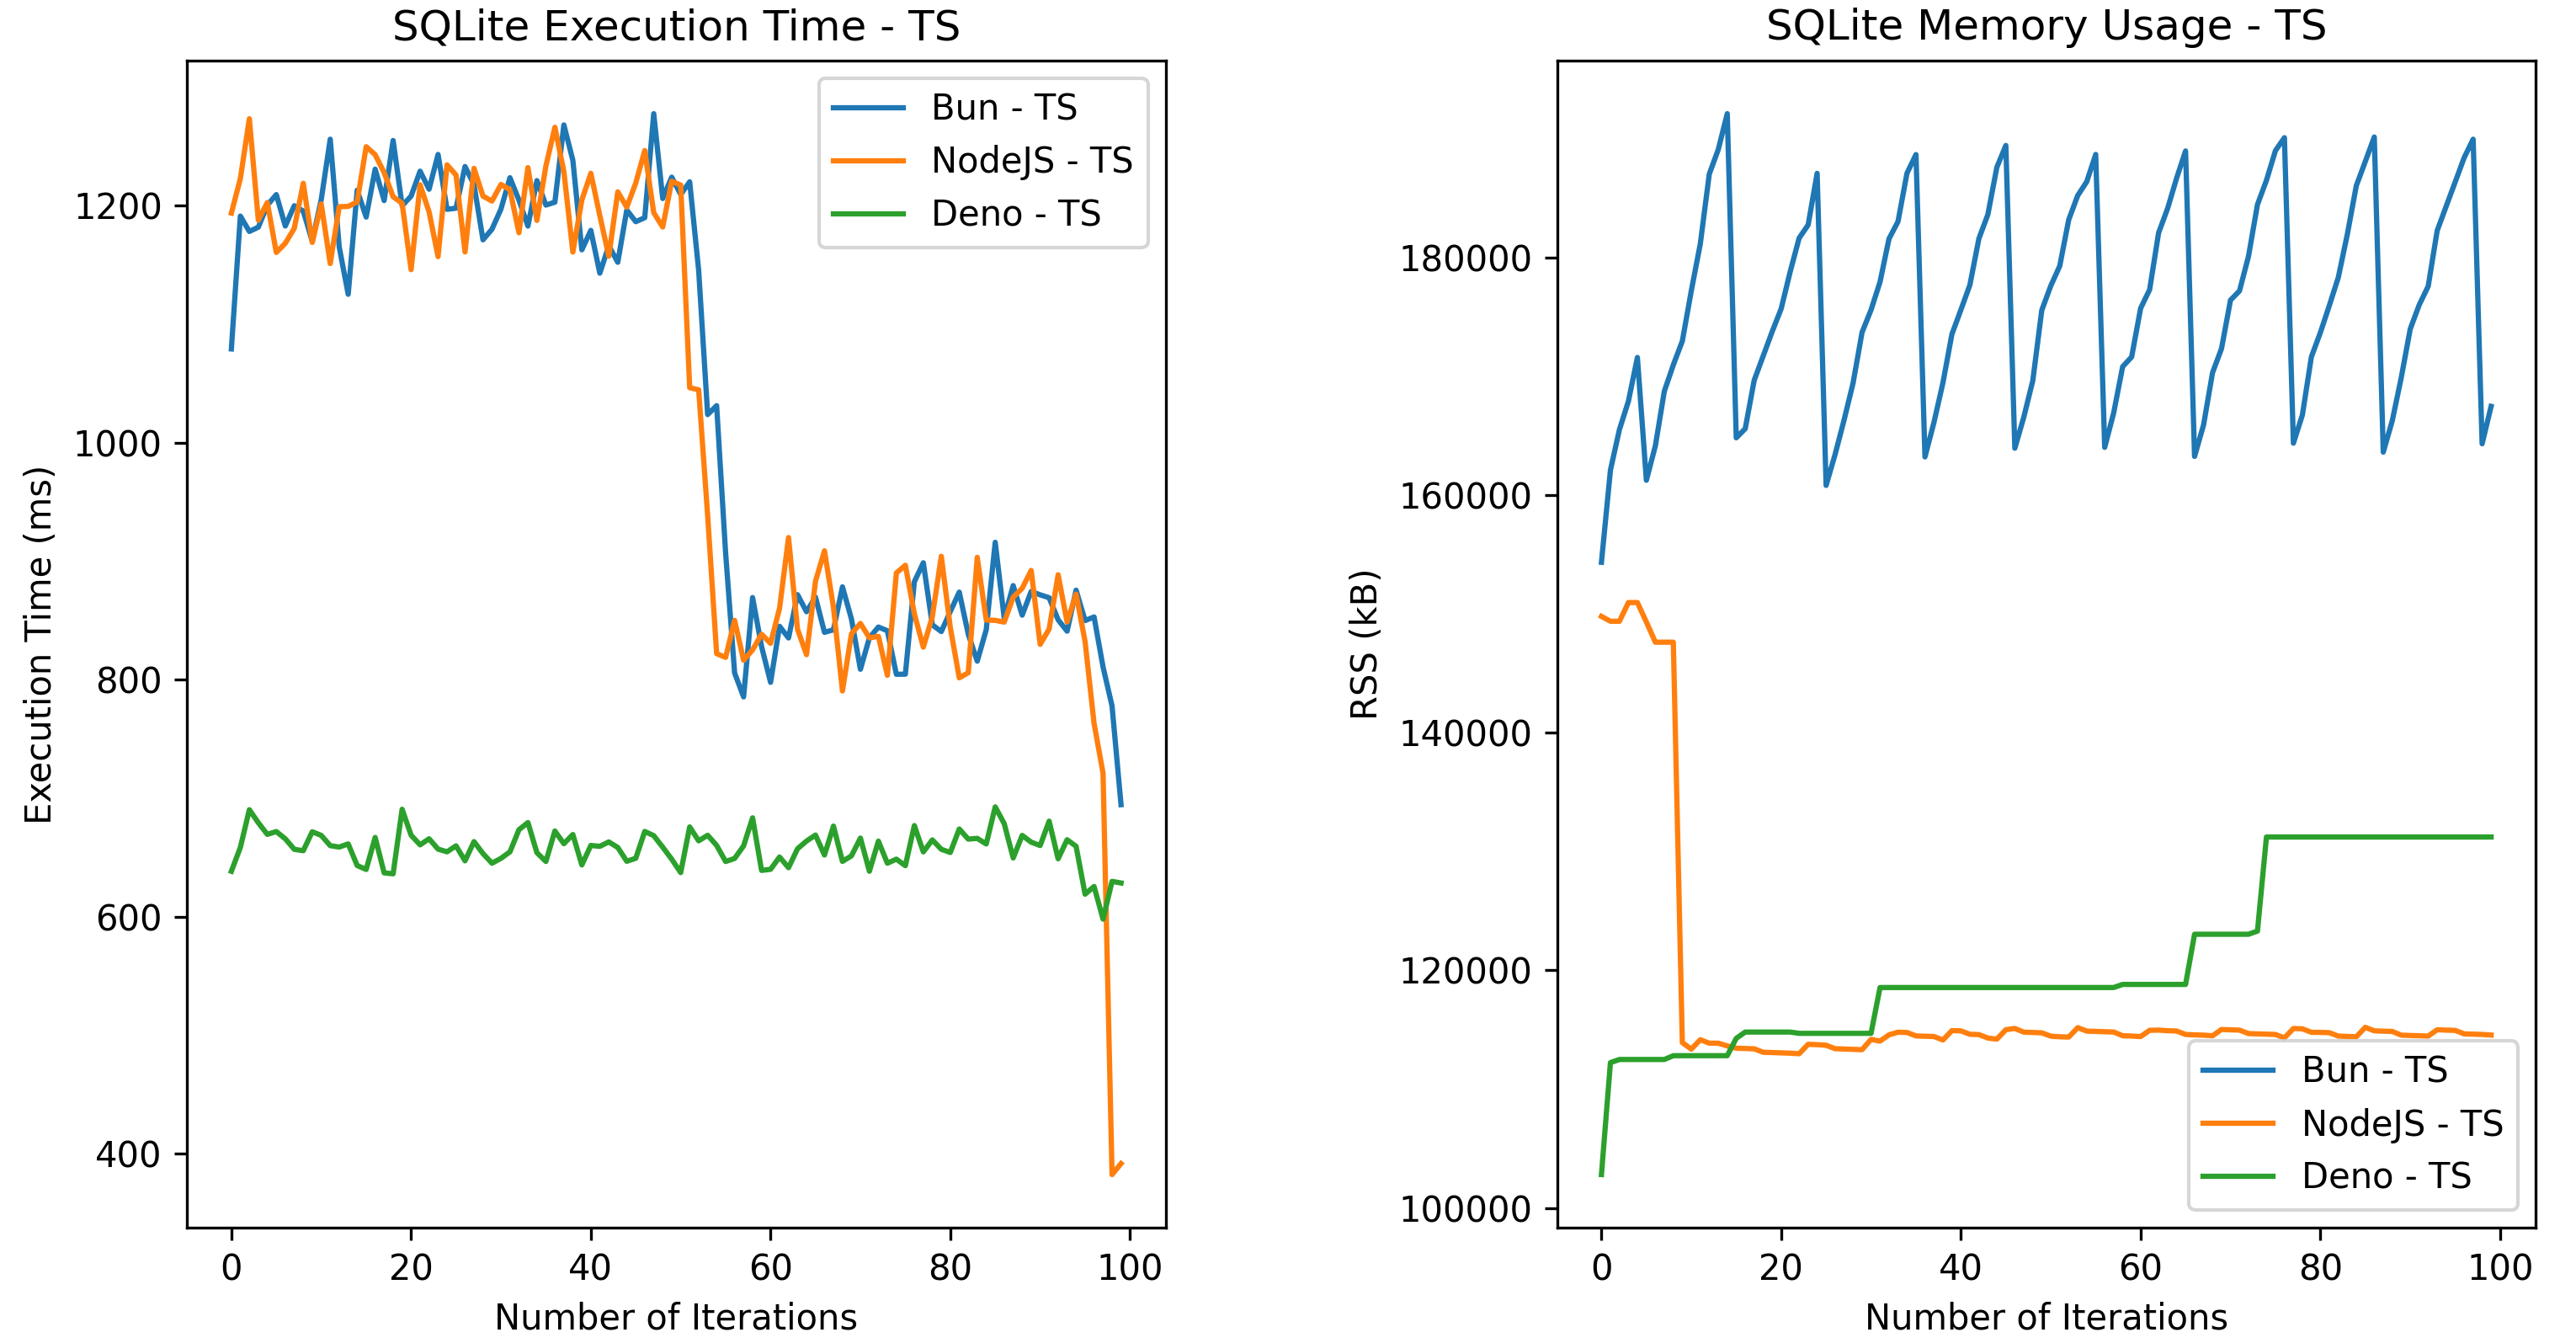
\includegraphics[width=0.7\textwidth]{Figures/database/sqlite_100_1000_ts.png}
  \caption{Wyniki eksperymentów dla testu bazy danych 100 iteracji oraz 1000 rekordów - po lewej czas wykonania jednorazowego testu w milisekundach, po prawej ilość zajmowanej pamięci w kilobajtach (kB)}
  \label{fig:database_e2_ts}
\end{figure}